\section{Example Results}

This section presents example results for different configurations of the Generalized Orthogonal Vectors Generator and Visualizer. It shows the generated vectors and their visualizations for various parameter values.

\subsection{Default Configuration}

The default configuration generates three orthogonal vectors from the origin [0, 0, 0] with a distance parameter of 1.0 and an angle parameter of $\pi/4$.

\subsubsection{Vector Coordinates}

The coordinates of the generated vectors are:

\begin{align}
\vec{R}_1 &= \begin{pmatrix} 0.8165 \\ -0.4082 \\ -0.4082 \end{pmatrix} \\
\vec{R}_2 &= \begin{pmatrix} 0.5774 \\ 0.5774 \\ 0.5774 \end{pmatrix} \\
\vec{R}_3 &= \begin{pmatrix} 0 \\ -0.7071 \\ 0.7071 \end{pmatrix}
\end{align}

\subsubsection{Dot Products}

The dot products between the displacement vectors are:

\begin{align}
\vec{v}_1 \cdot \vec{v}_2 &= 0 \\
\vec{v}_1 \cdot \vec{v}_3 &= 0 \\
\vec{v}_2 \cdot \vec{v}_3 &= 0
\end{align}

These dot products confirm that the vectors are orthogonal.

\subsubsection{3D Visualization}

\begin{figure}[H]
    \centering
    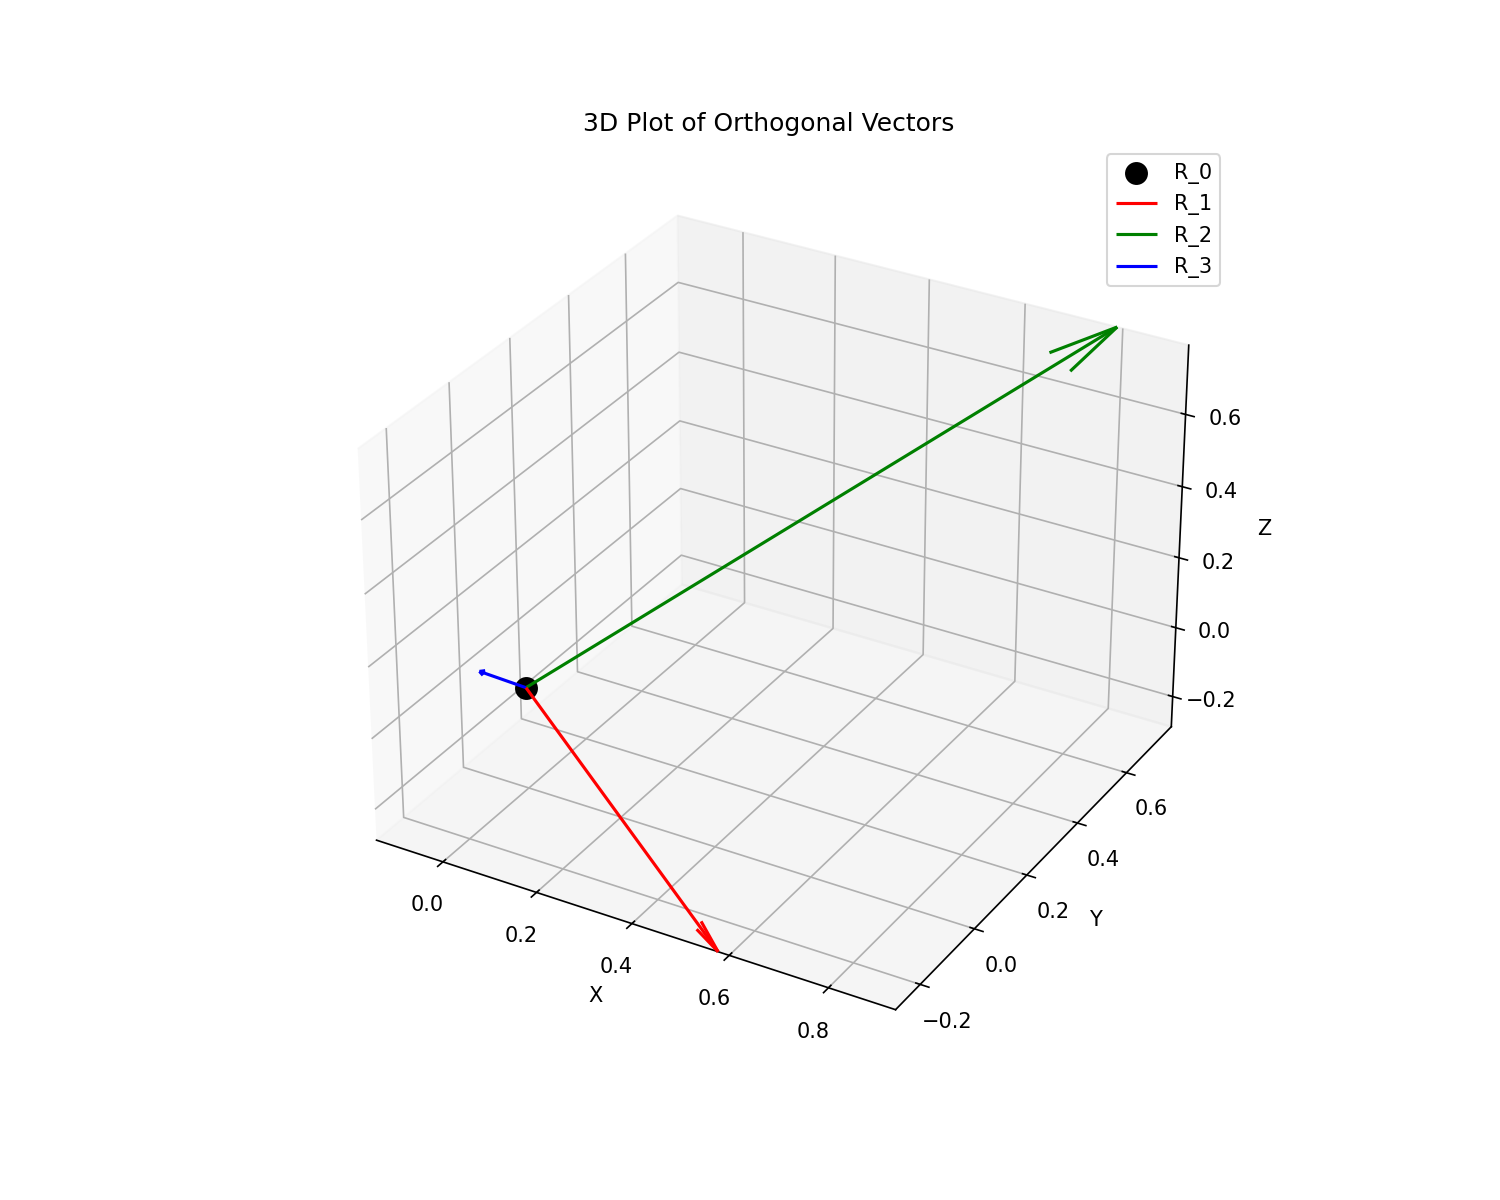
\includegraphics[width=0.8\textwidth]{figures/default_3d.png}
    \caption{3D visualization of the default configuration}
    \label{fig:example_default_3d}
\end{figure}

\subsubsection{2D Projections}

\begin{figure}[H]
    \centering
    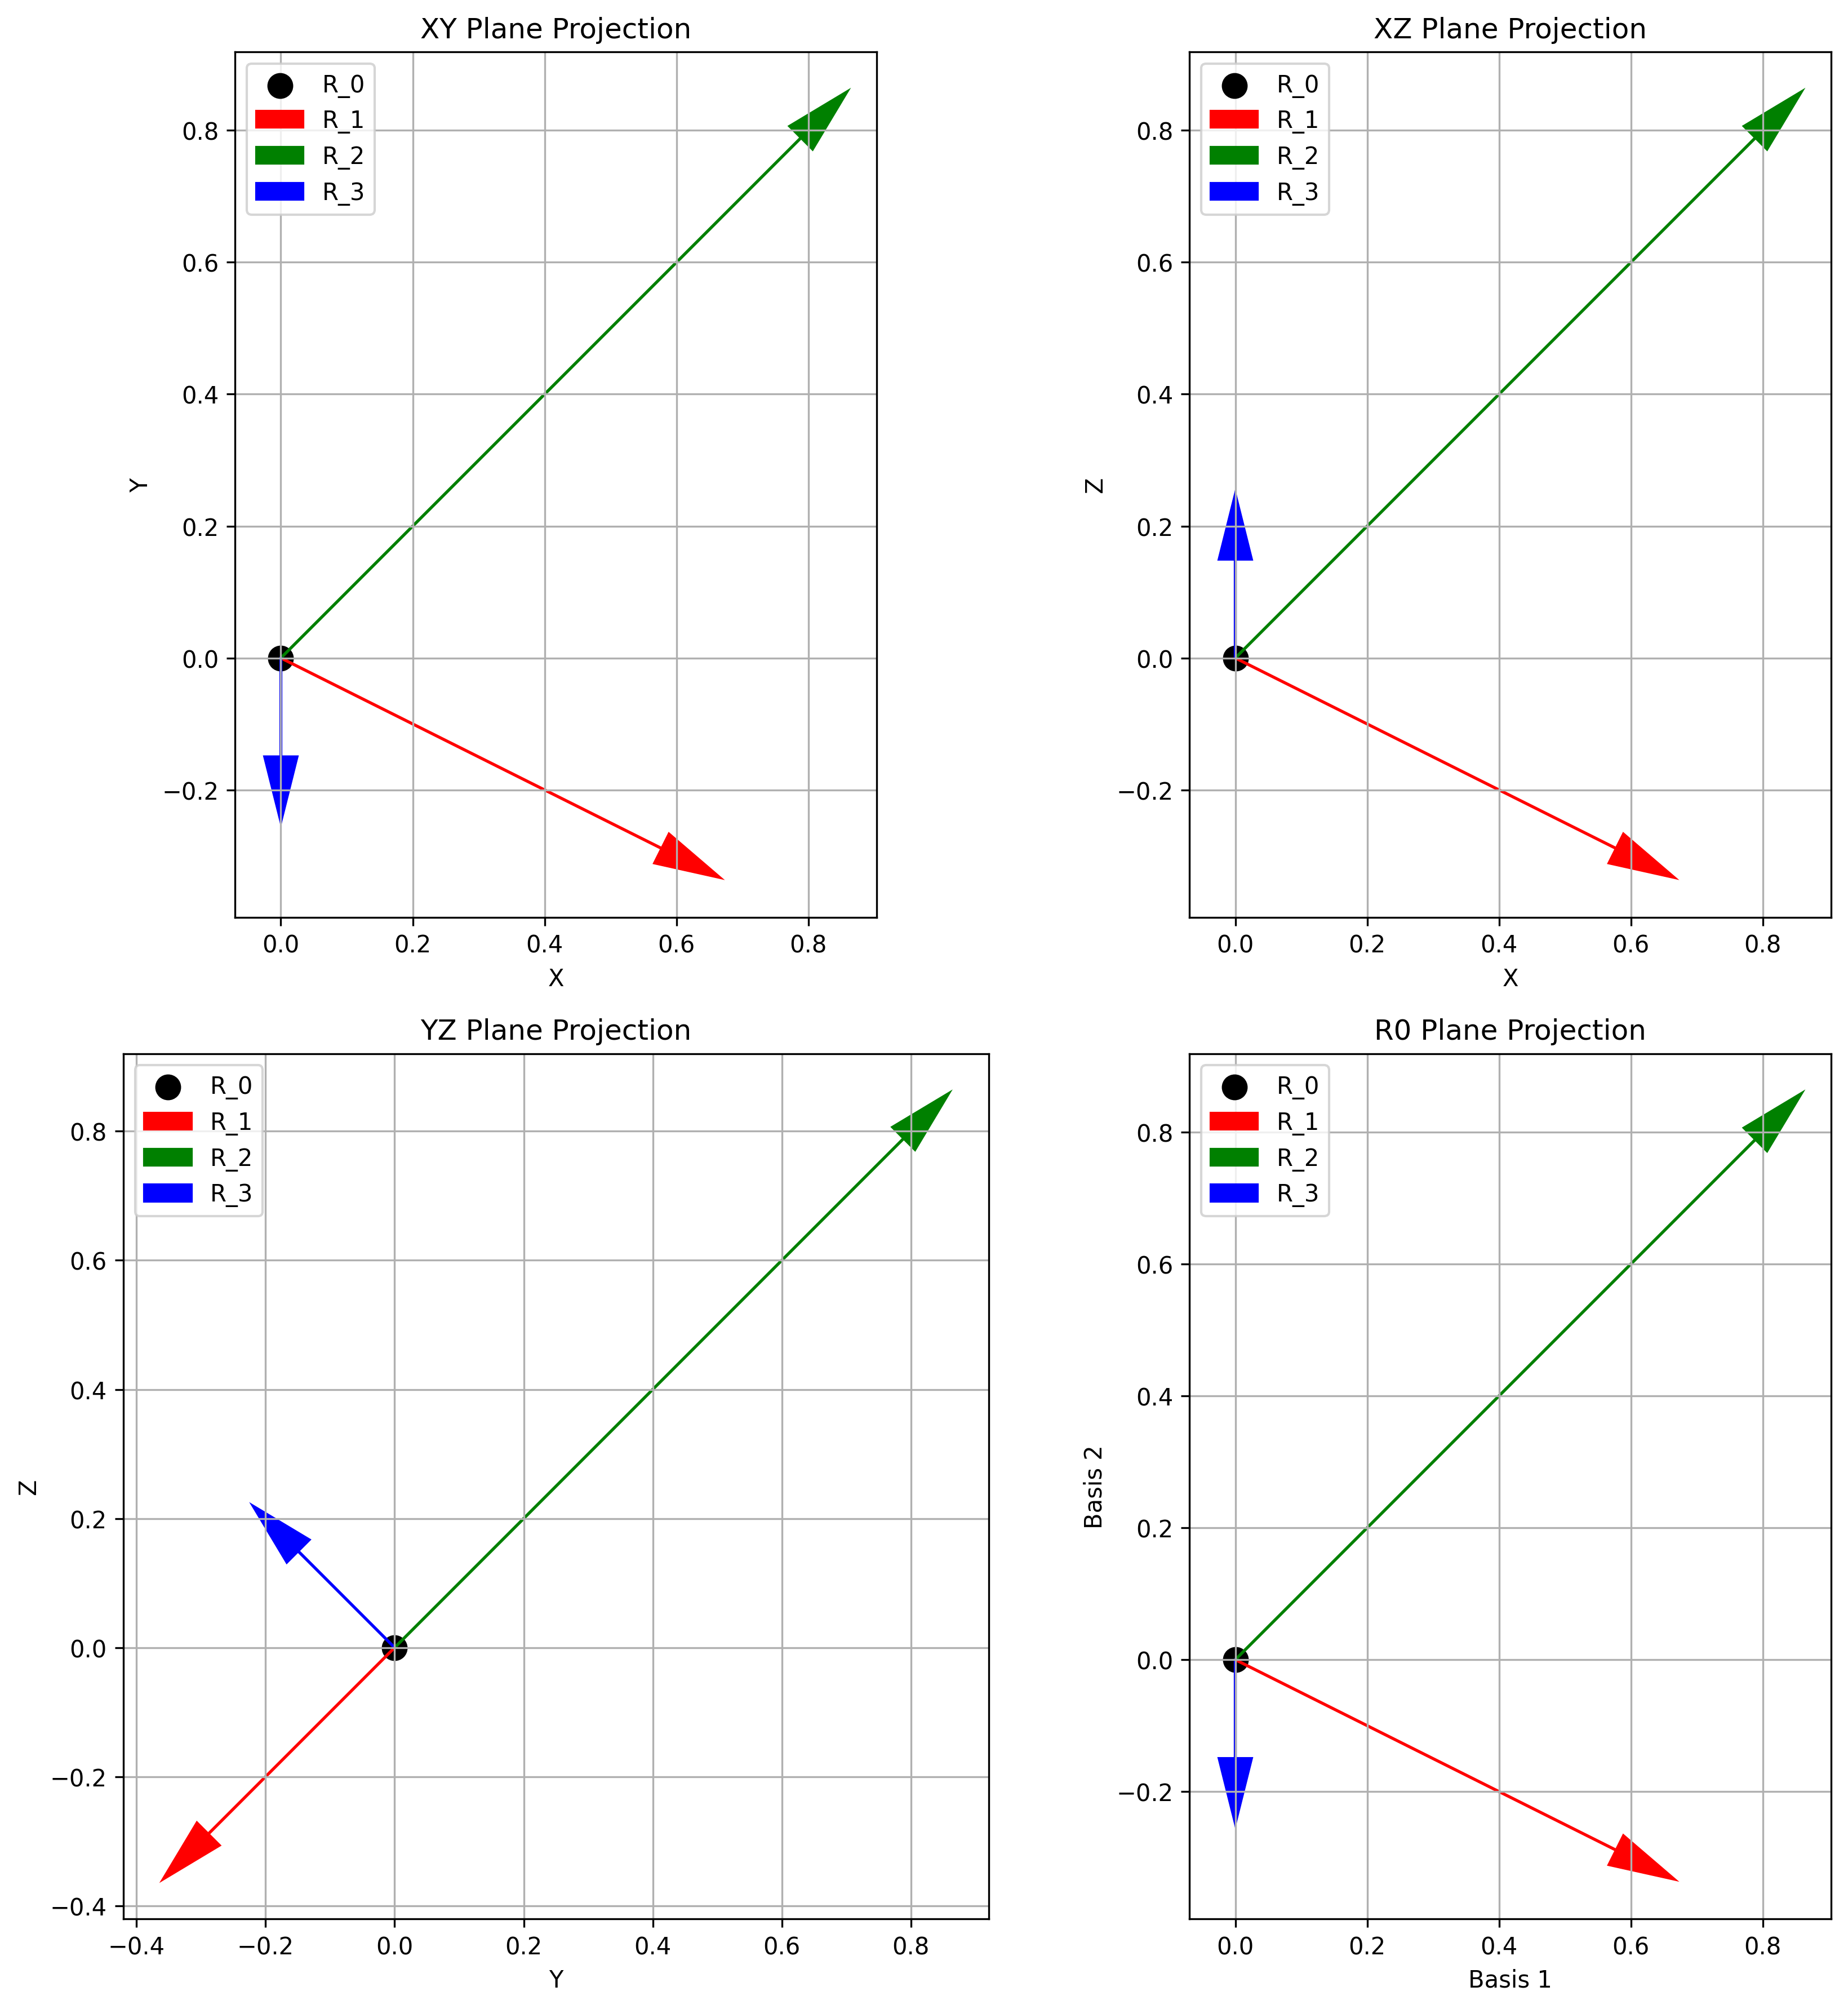
\includegraphics[width=0.8\textwidth]{figures/2d_projections.png}
    \caption{2D projections of the default configuration}
    \label{fig:example_default_2d}
\end{figure}

\subsection{Custom Configuration 1}

This configuration generates three orthogonal vectors from the origin [1, 1, 1] with a distance parameter of 2.0 and an angle parameter of $\pi/3$.

\subsubsection{Vector Coordinates}

The coordinates of the generated vectors are:

\begin{align}
\vec{R}_1 &= \begin{pmatrix} 2.6330 \\ 0.3165 \\ 0.3165 \end{pmatrix} \\
\vec{R}_2 &= \begin{pmatrix} 1.6667 \\ 1.6667 \\ 1.6667 \end{pmatrix} \\
\vec{R}_3 &= \begin{pmatrix} 1 \\ -0.1547 \\ 2.1547 \end{pmatrix}
\end{align}

\subsubsection{Dot Products}

The dot products between the displacement vectors are:

\begin{align}
\vec{v}_1 \cdot \vec{v}_2 &= 0 \\
\vec{v}_1 \cdot \vec{v}_3 &= 0 \\
\vec{v}_2 \cdot \vec{v}_3 &= 0
\end{align}

These dot products confirm that the vectors are orthogonal.

\subsubsection{3D Visualization}

\begin{figure}[H]
    \centering
    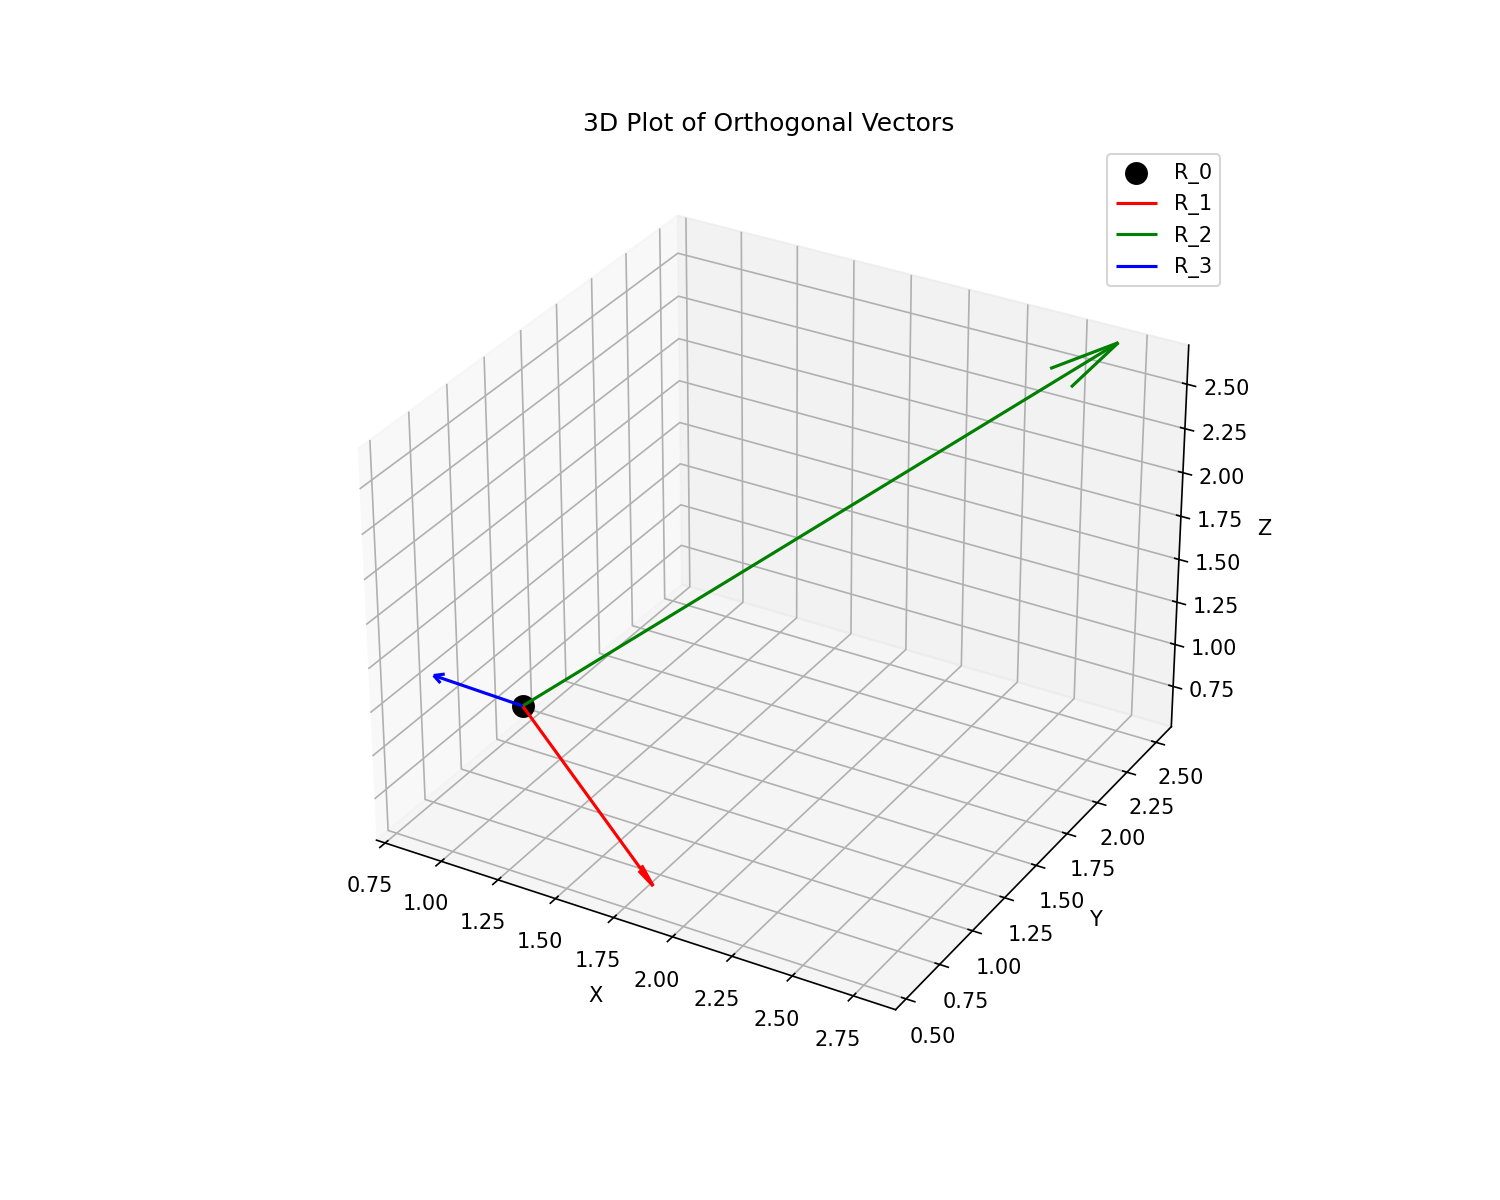
\includegraphics[width=0.8\textwidth]{figures/custom1_3d.png}
    \caption{3D visualization of custom configuration 1}
    \label{fig:example_custom1_3d}
\end{figure}

\subsubsection{2D Projections}

\begin{figure}[H]
    \centering
    \begin{minipage}{0.48\textwidth}
        \centering
        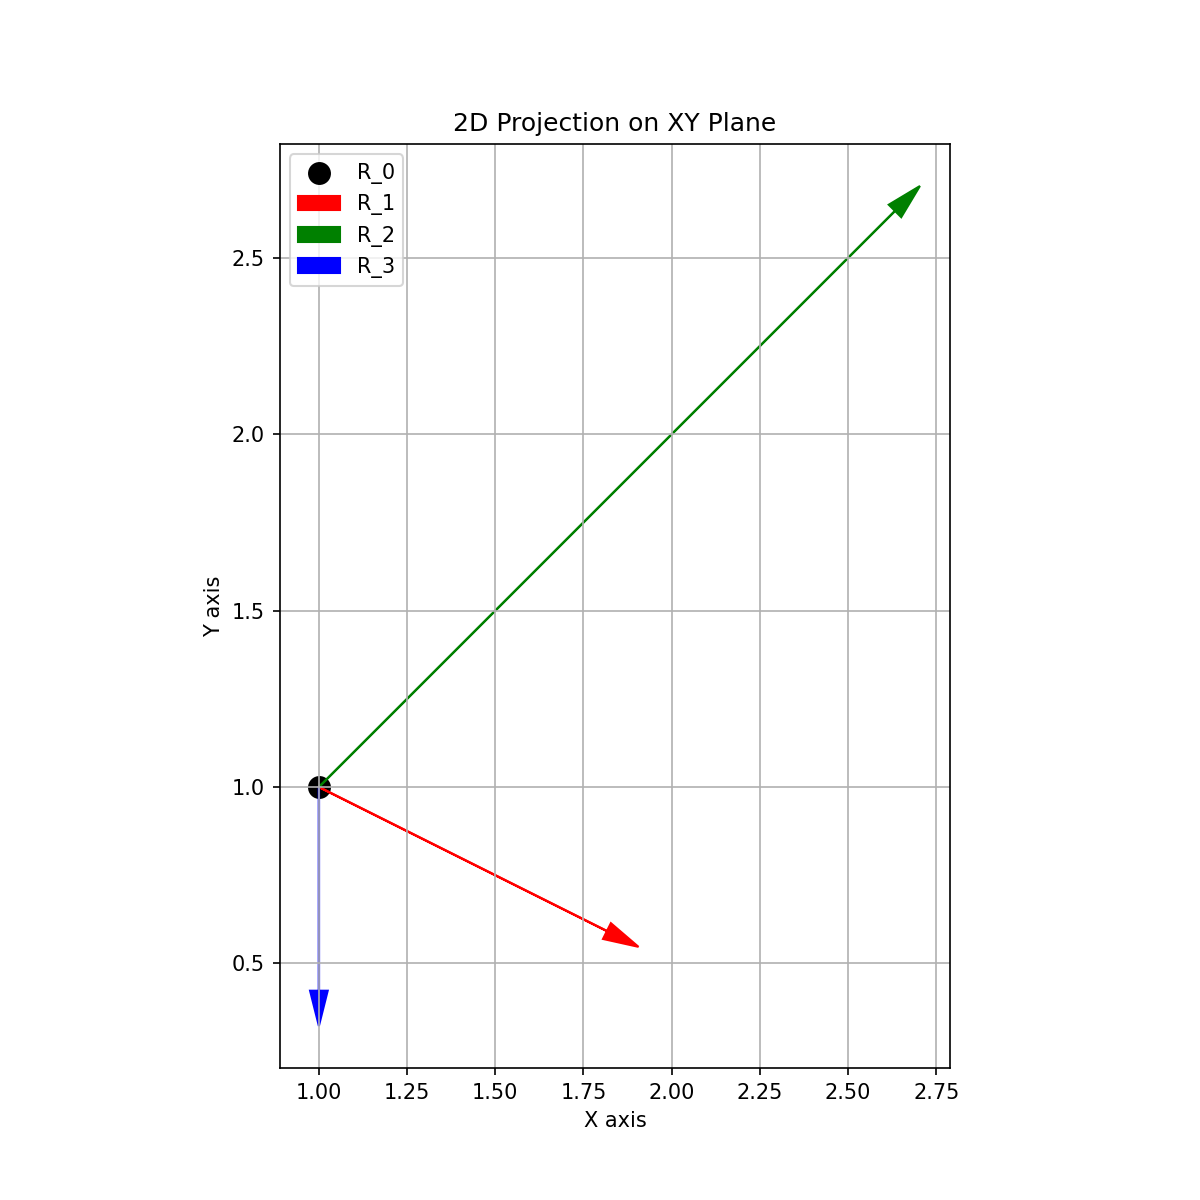
\includegraphics[width=\textwidth]{figures/custom1_xy.png}
        \caption*{XY Projection}
    \end{minipage}\hfill
    \begin{minipage}{0.48\textwidth}
        \centering
        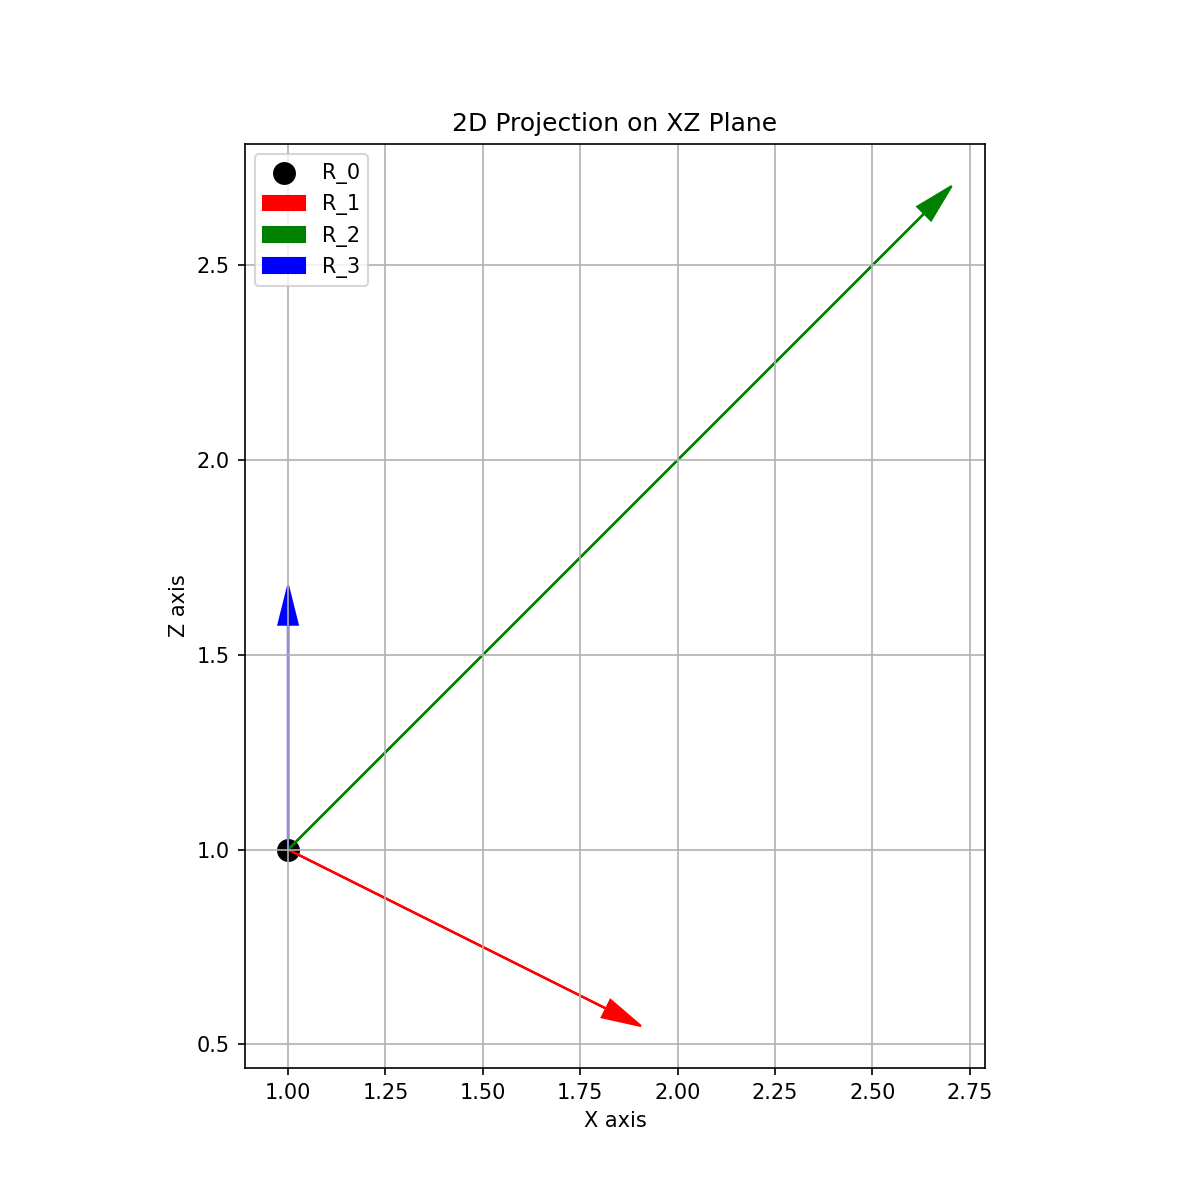
\includegraphics[width=\textwidth]{figures/custom1_xz.png}
        \caption*{XZ Projection}
    \end{minipage}
    
    \begin{minipage}{0.48\textwidth}
        \centering
        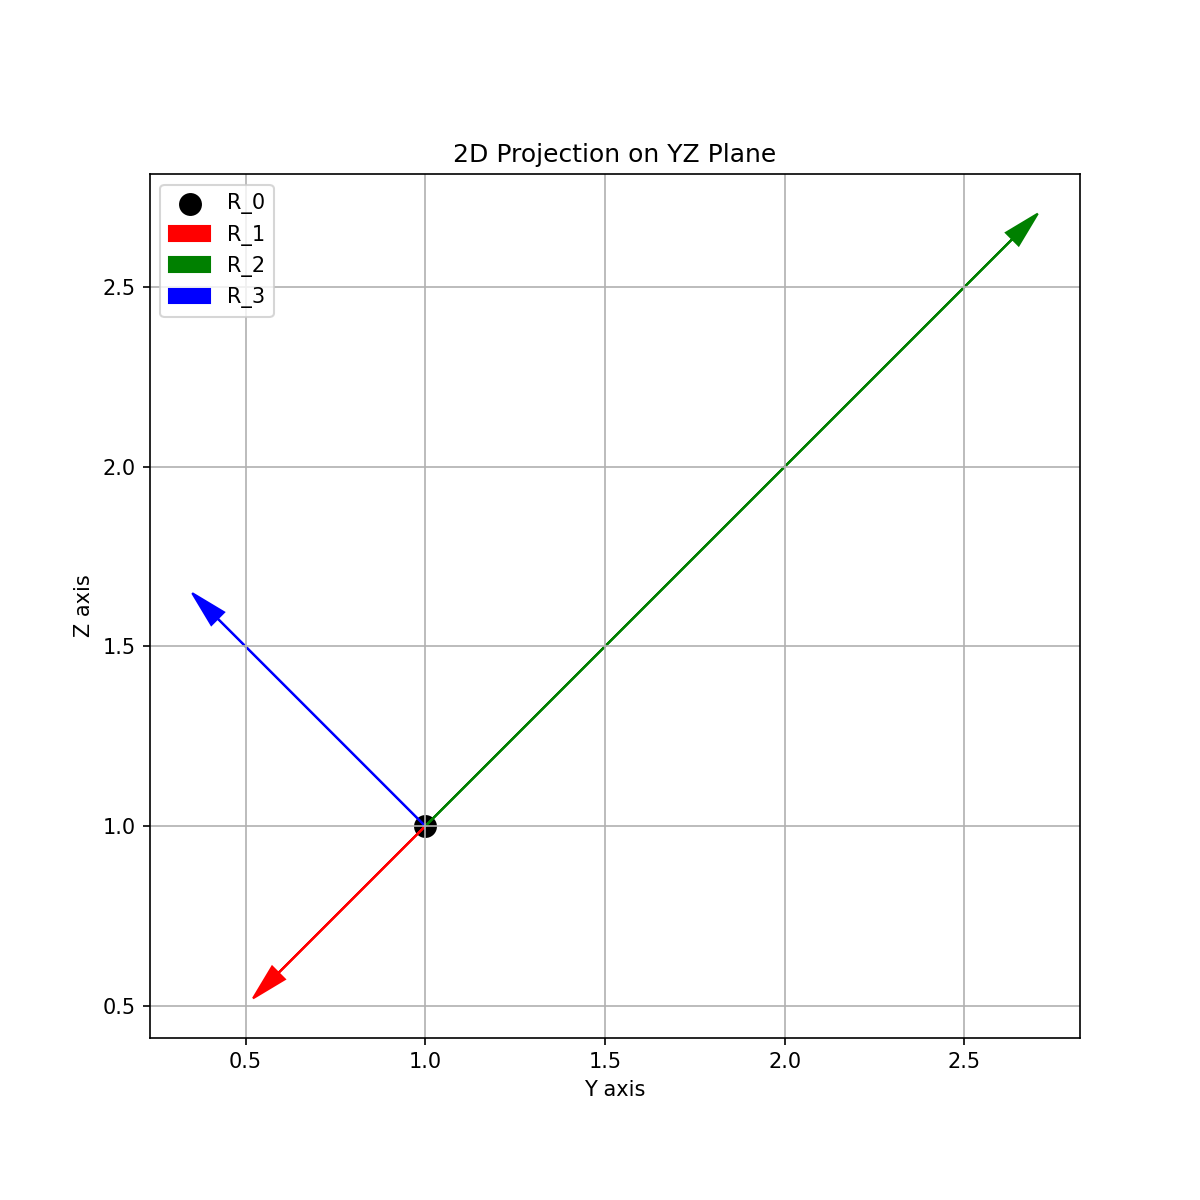
\includegraphics[width=\textwidth]{figures/custom1_yz.png}
        \caption*{YZ Projection}
    \end{minipage}\hfill
    \begin{minipage}{0.48\textwidth}
        \centering
        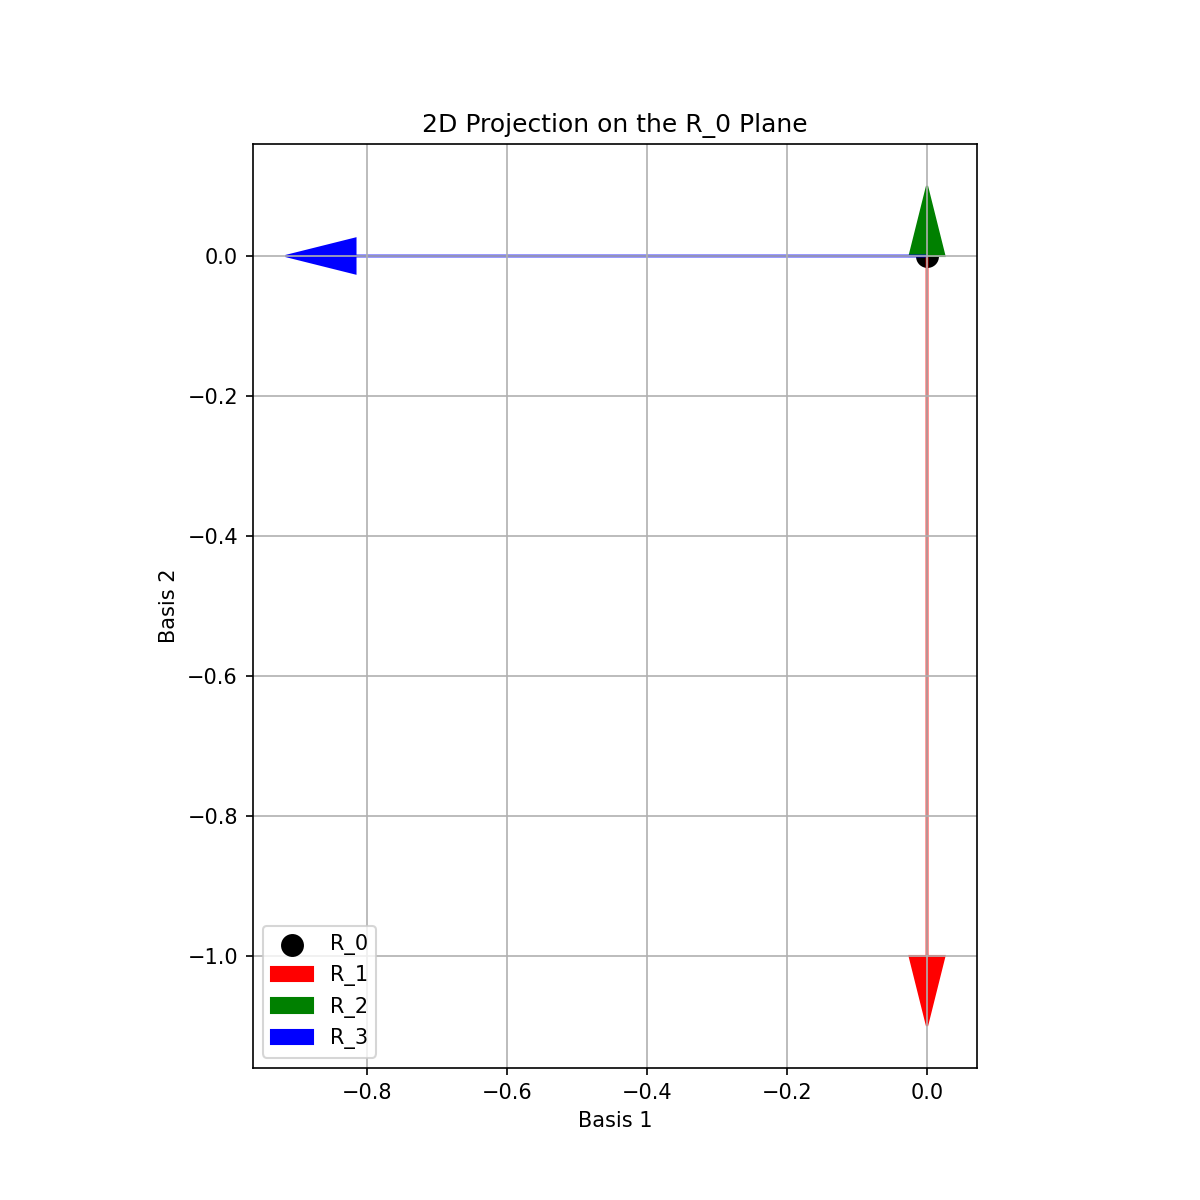
\includegraphics[width=\textwidth]{figures/custom1_r0.png}
        \caption*{R0 Projection}
    \end{minipage}
    \caption{2D projections of custom configuration 1}
    \label{fig:example_custom1_2d}
\end{figure}

\subsection{Custom Configuration 2}

This configuration generates three orthogonal vectors from the origin [0, 0, 2] with a distance parameter of 1.5 and an angle parameter of $\pi/6$.

\subsubsection{Vector Coordinates}

The coordinates of the generated vectors are:

\begin{align}
\vec{R}_1 &= \begin{pmatrix} 1.2990 \\ -0.6495 \\ 1.3505 \end{pmatrix} \\
\vec{R}_2 &= \begin{pmatrix} 0.7217 \\ 0.7217 \\ 2.7217 \end{pmatrix} \\
\vec{R}_3 &= \begin{pmatrix} 0 \\ -0.3750 \\ 2.3750 \end{pmatrix}
\end{align}

\subsubsection{Dot Products}

The dot products between the displacement vectors are:

\begin{align}
\vec{v}_1 \cdot \vec{v}_2 &= 0 \\
\vec{v}_1 \cdot \vec{v}_3 &= 0 \\
\vec{v}_2 \cdot \vec{v}_3 &= 0
\end{align}

These dot products confirm that the vectors are orthogonal.

\subsubsection{3D Visualization}

\begin{figure}[H]
    \centering
    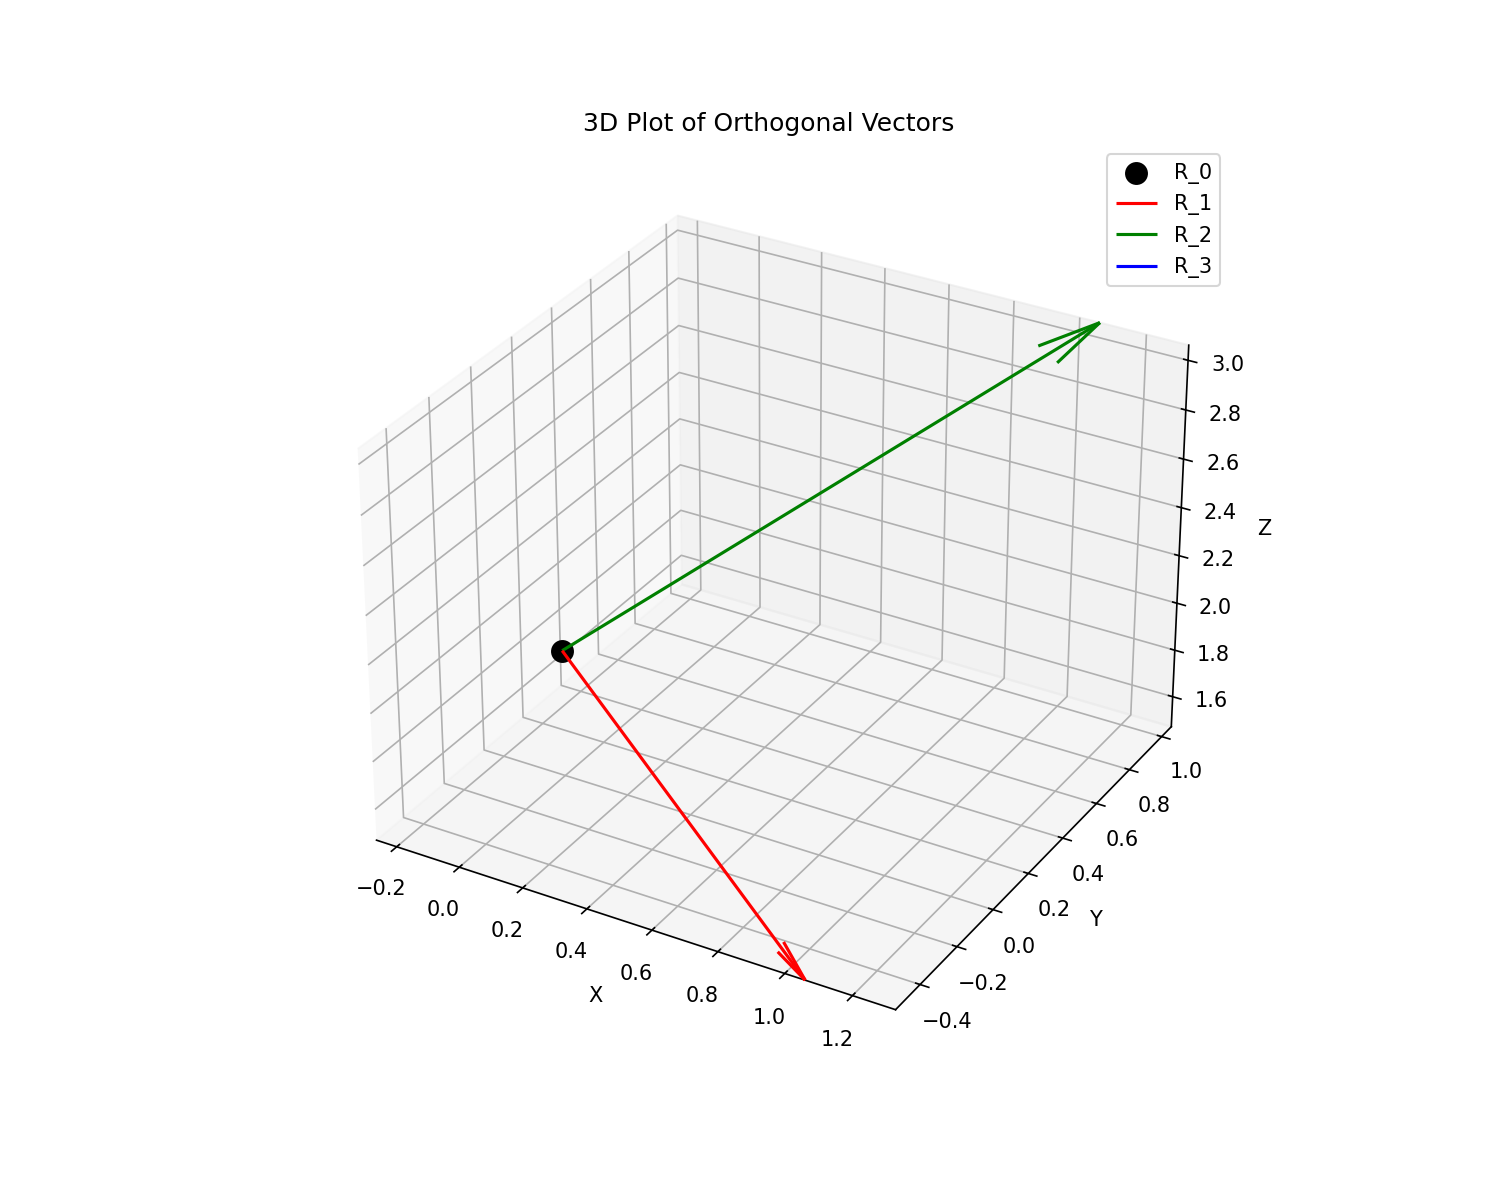
\includegraphics[width=0.8\textwidth]{figures/custom2_3d.png}
    \caption{3D visualization of custom configuration 2}
    \label{fig:example_custom2_3d}
\end{figure}

\subsubsection{2D Projections}

\begin{figure}[H]
    \centering
    \begin{minipage}{0.48\textwidth}
        \centering
        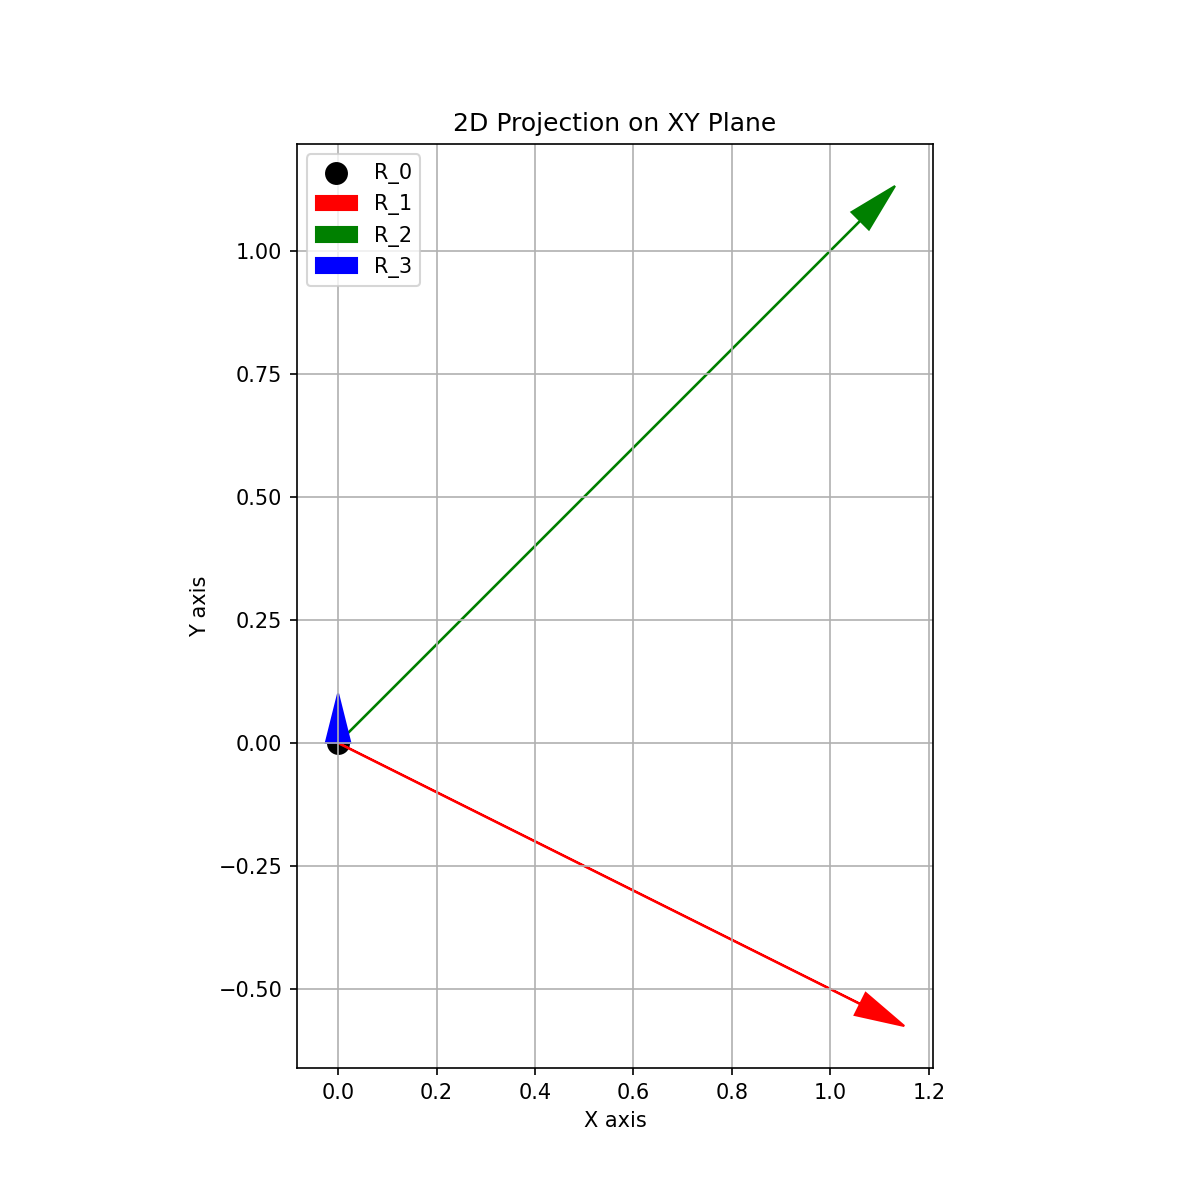
\includegraphics[width=\textwidth]{figures/custom2_xy.png}
        \caption*{XY Projection}
    \end{minipage}\hfill
    \begin{minipage}{0.48\textwidth}
        \centering
        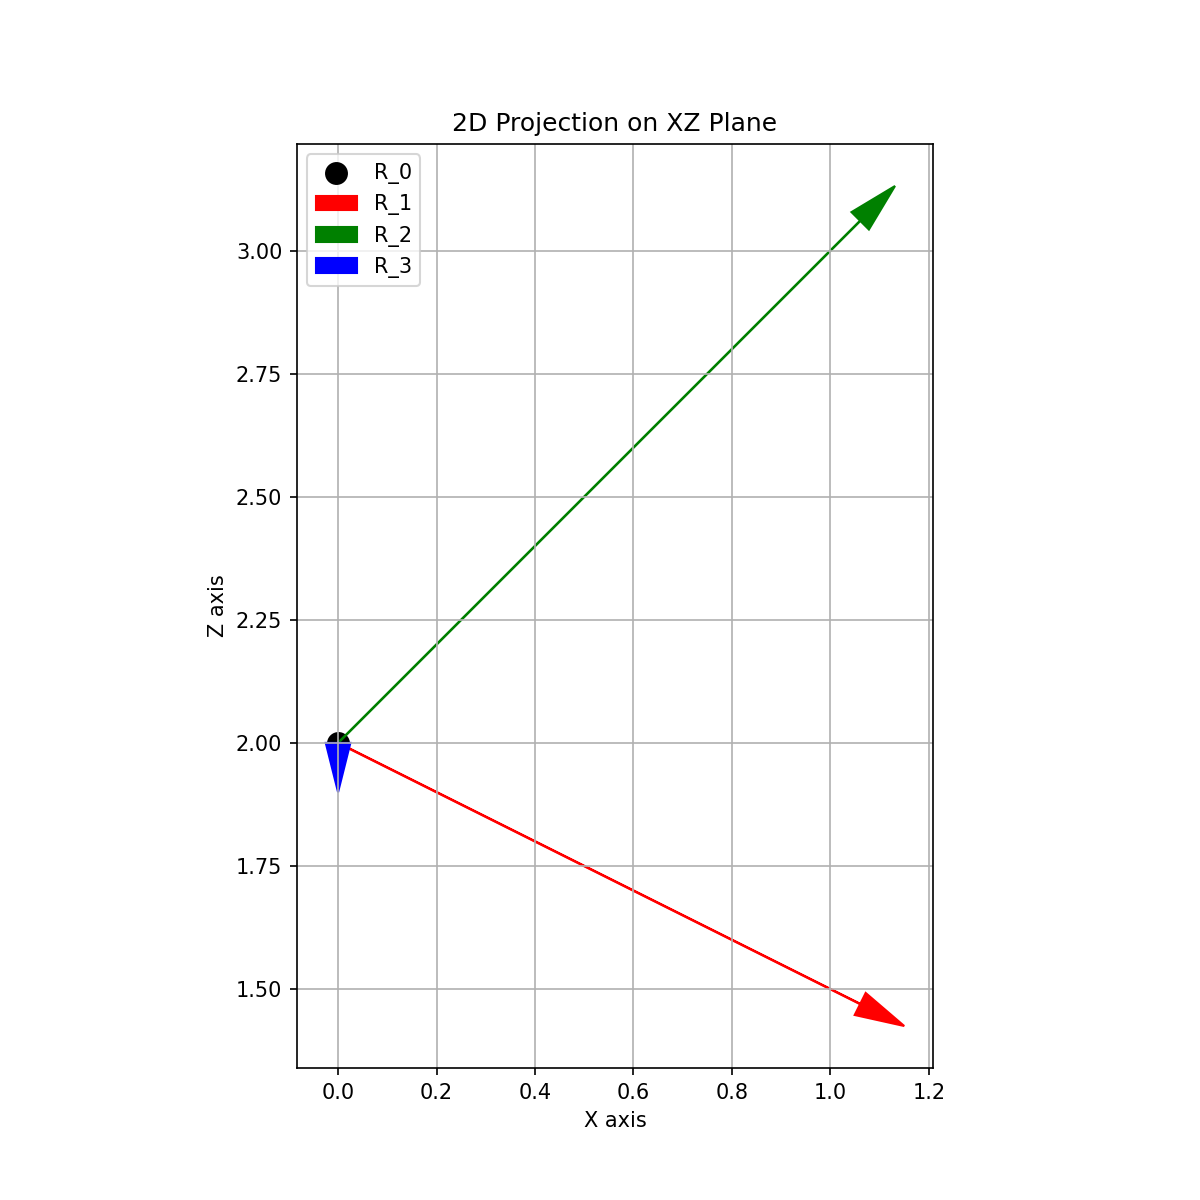
\includegraphics[width=\textwidth]{figures/custom2_xz.png}
        \caption*{XZ Projection}
    \end{minipage}
    
    \begin{minipage}{0.48\textwidth}
        \centering
        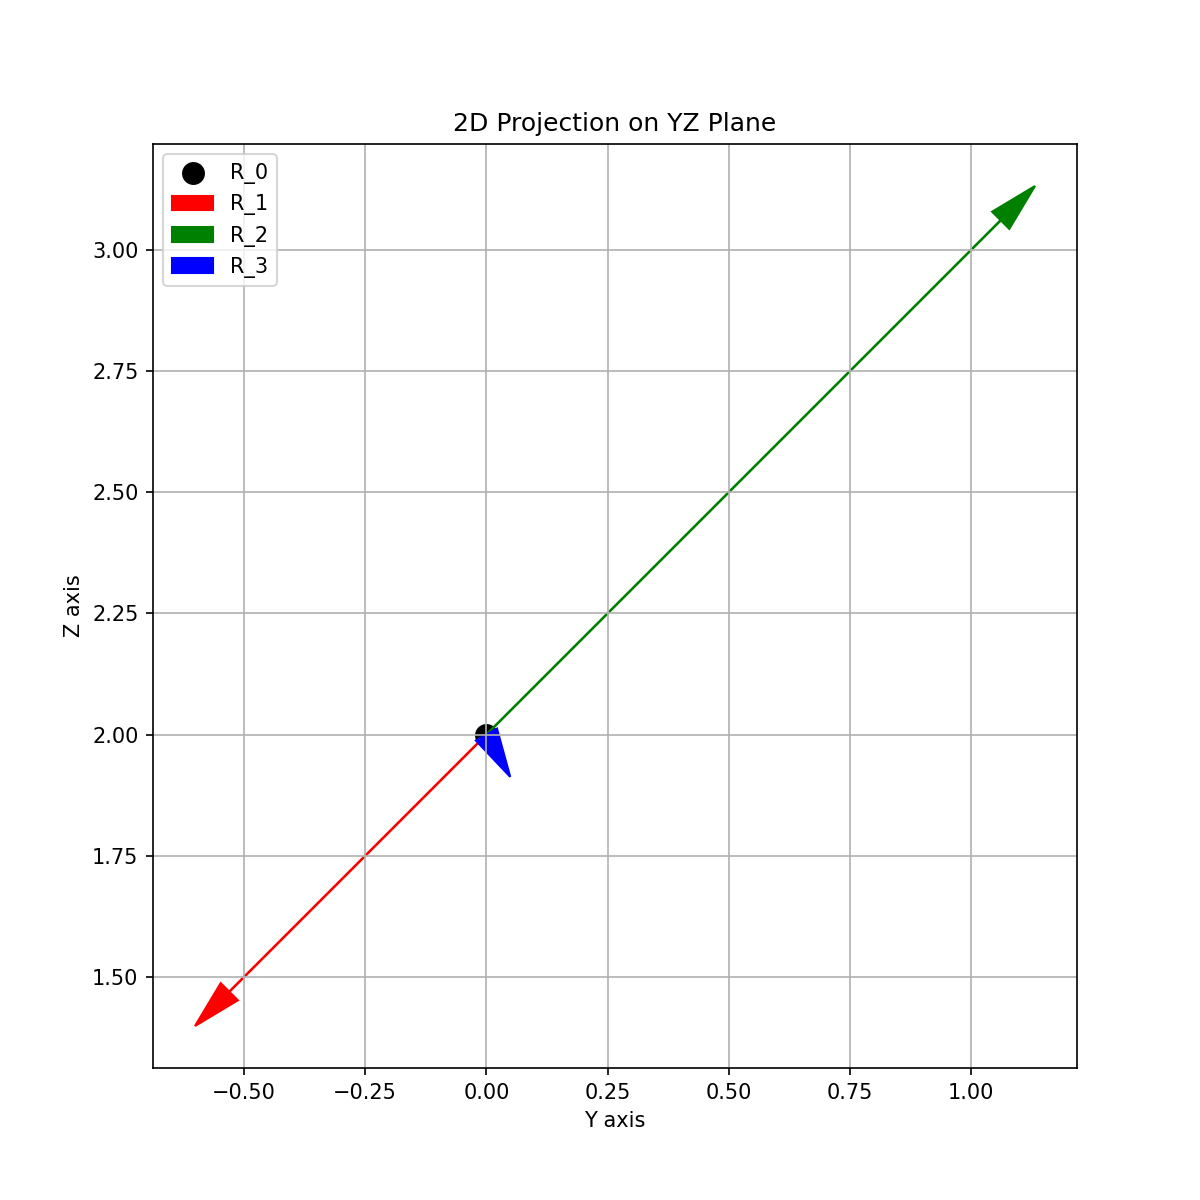
\includegraphics[width=\textwidth]{figures/custom2_yz.png}
        \caption*{YZ Projection}
    \end{minipage}\hfill
    \begin{minipage}{0.48\textwidth}
        \centering
        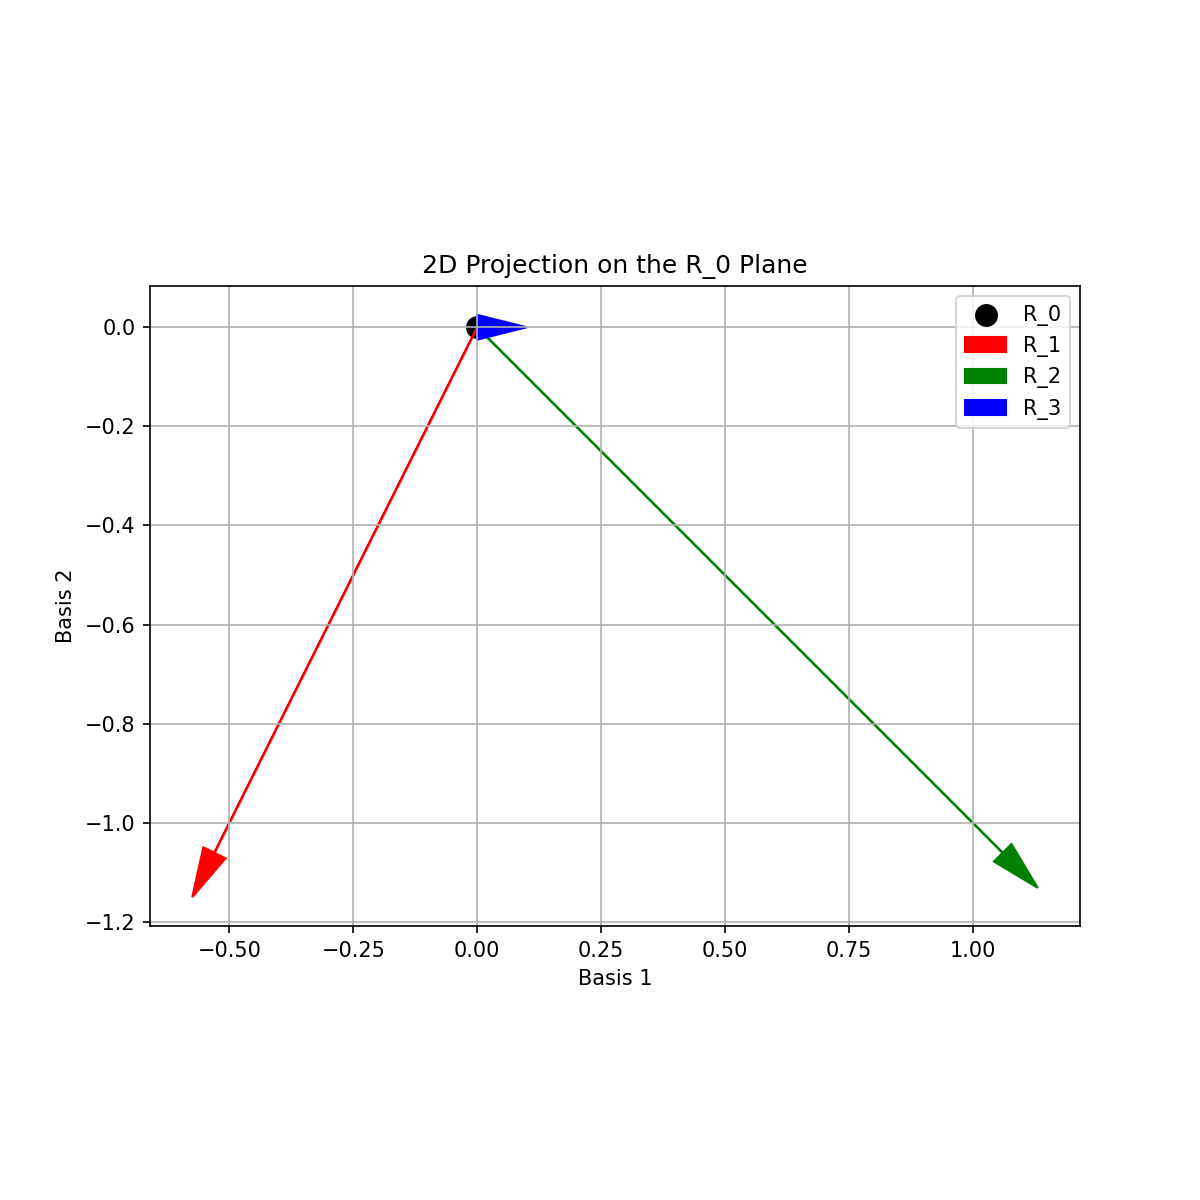
\includegraphics[width=\textwidth]{figures/custom2_r0.png}
        \caption*{R0 Projection}
    \end{minipage}
    \caption{2D projections of custom configuration 2}
    \label{fig:example_custom2_2d}
\end{figure}

\subsection{Effect of Distance Parameter}

The distance parameter $d$ scales the vectors equally, preserving their orthogonality. Increasing $d$ increases the distance of the vectors from the origin, while decreasing $d$ decreases the distance.

\begin{figure}[H]
    \centering
    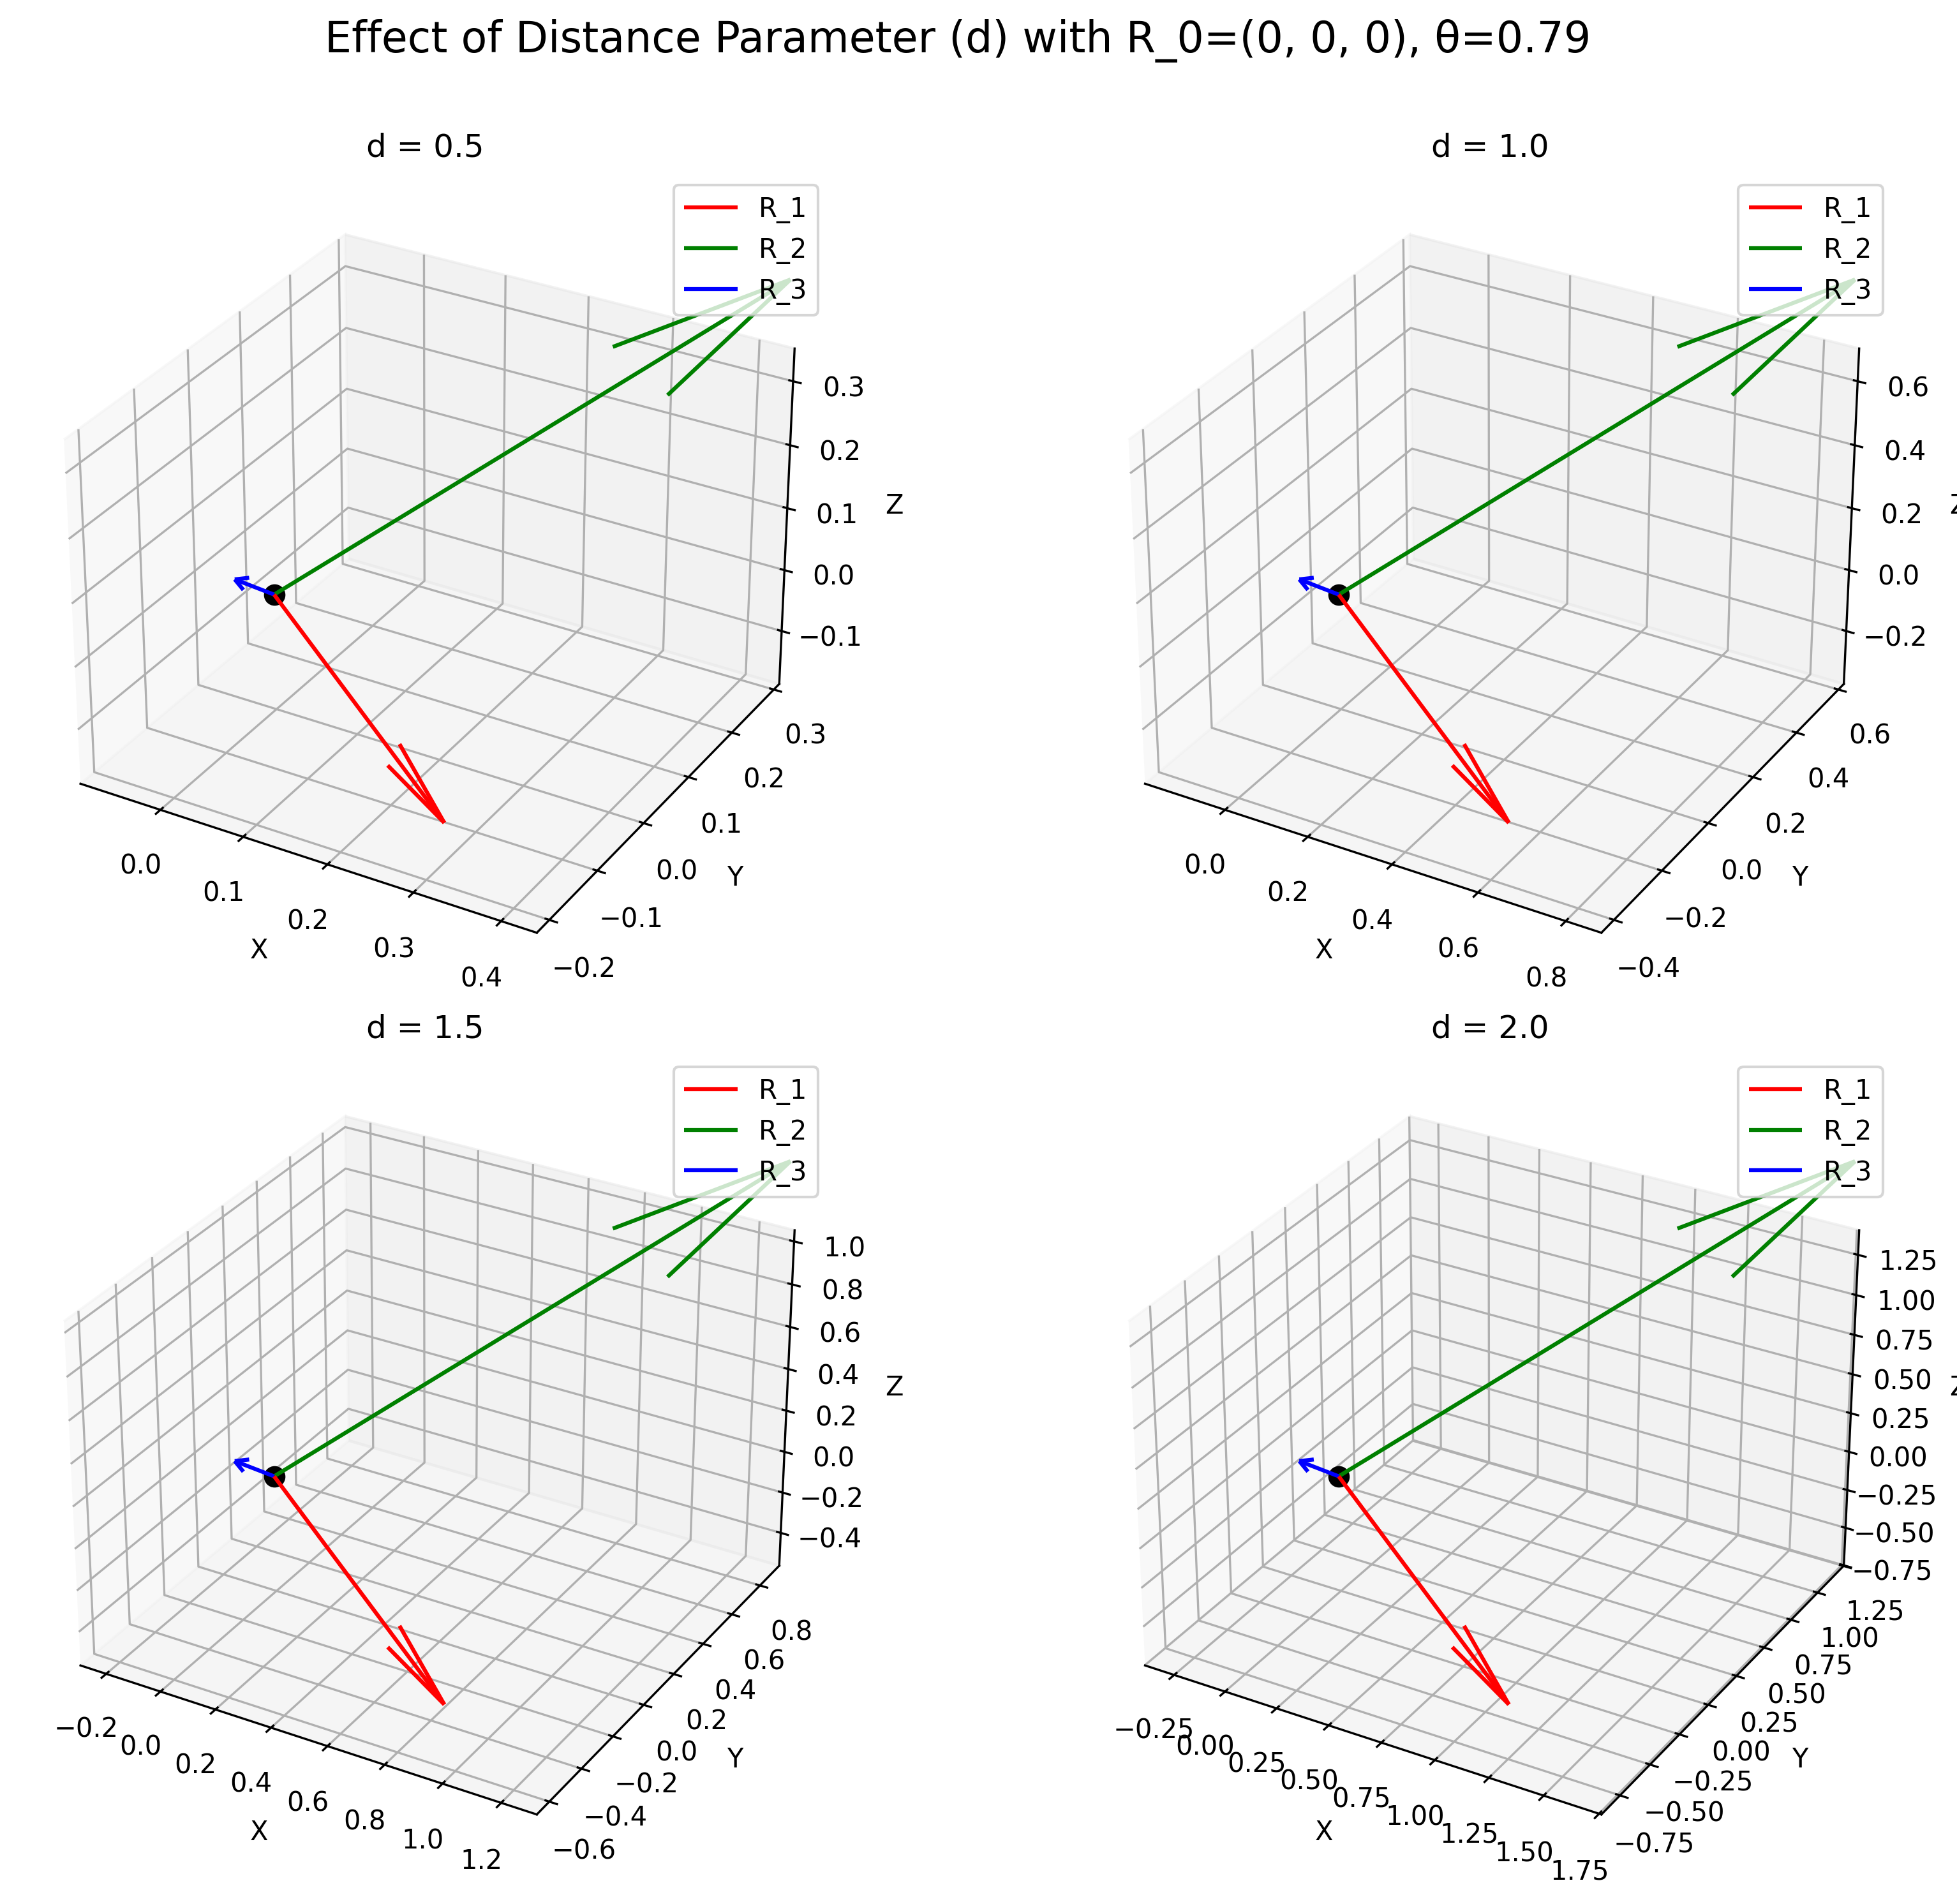
\includegraphics[width=0.9\textwidth]{figures/d_effect_R0_0_0_0.png}
    \caption{Effect of distance parameter on vector visualization with origin at $(0,0,0)$}
    \label{fig:example_distance_effect_default}
\end{figure}

\begin{figure}[H]
    \centering
    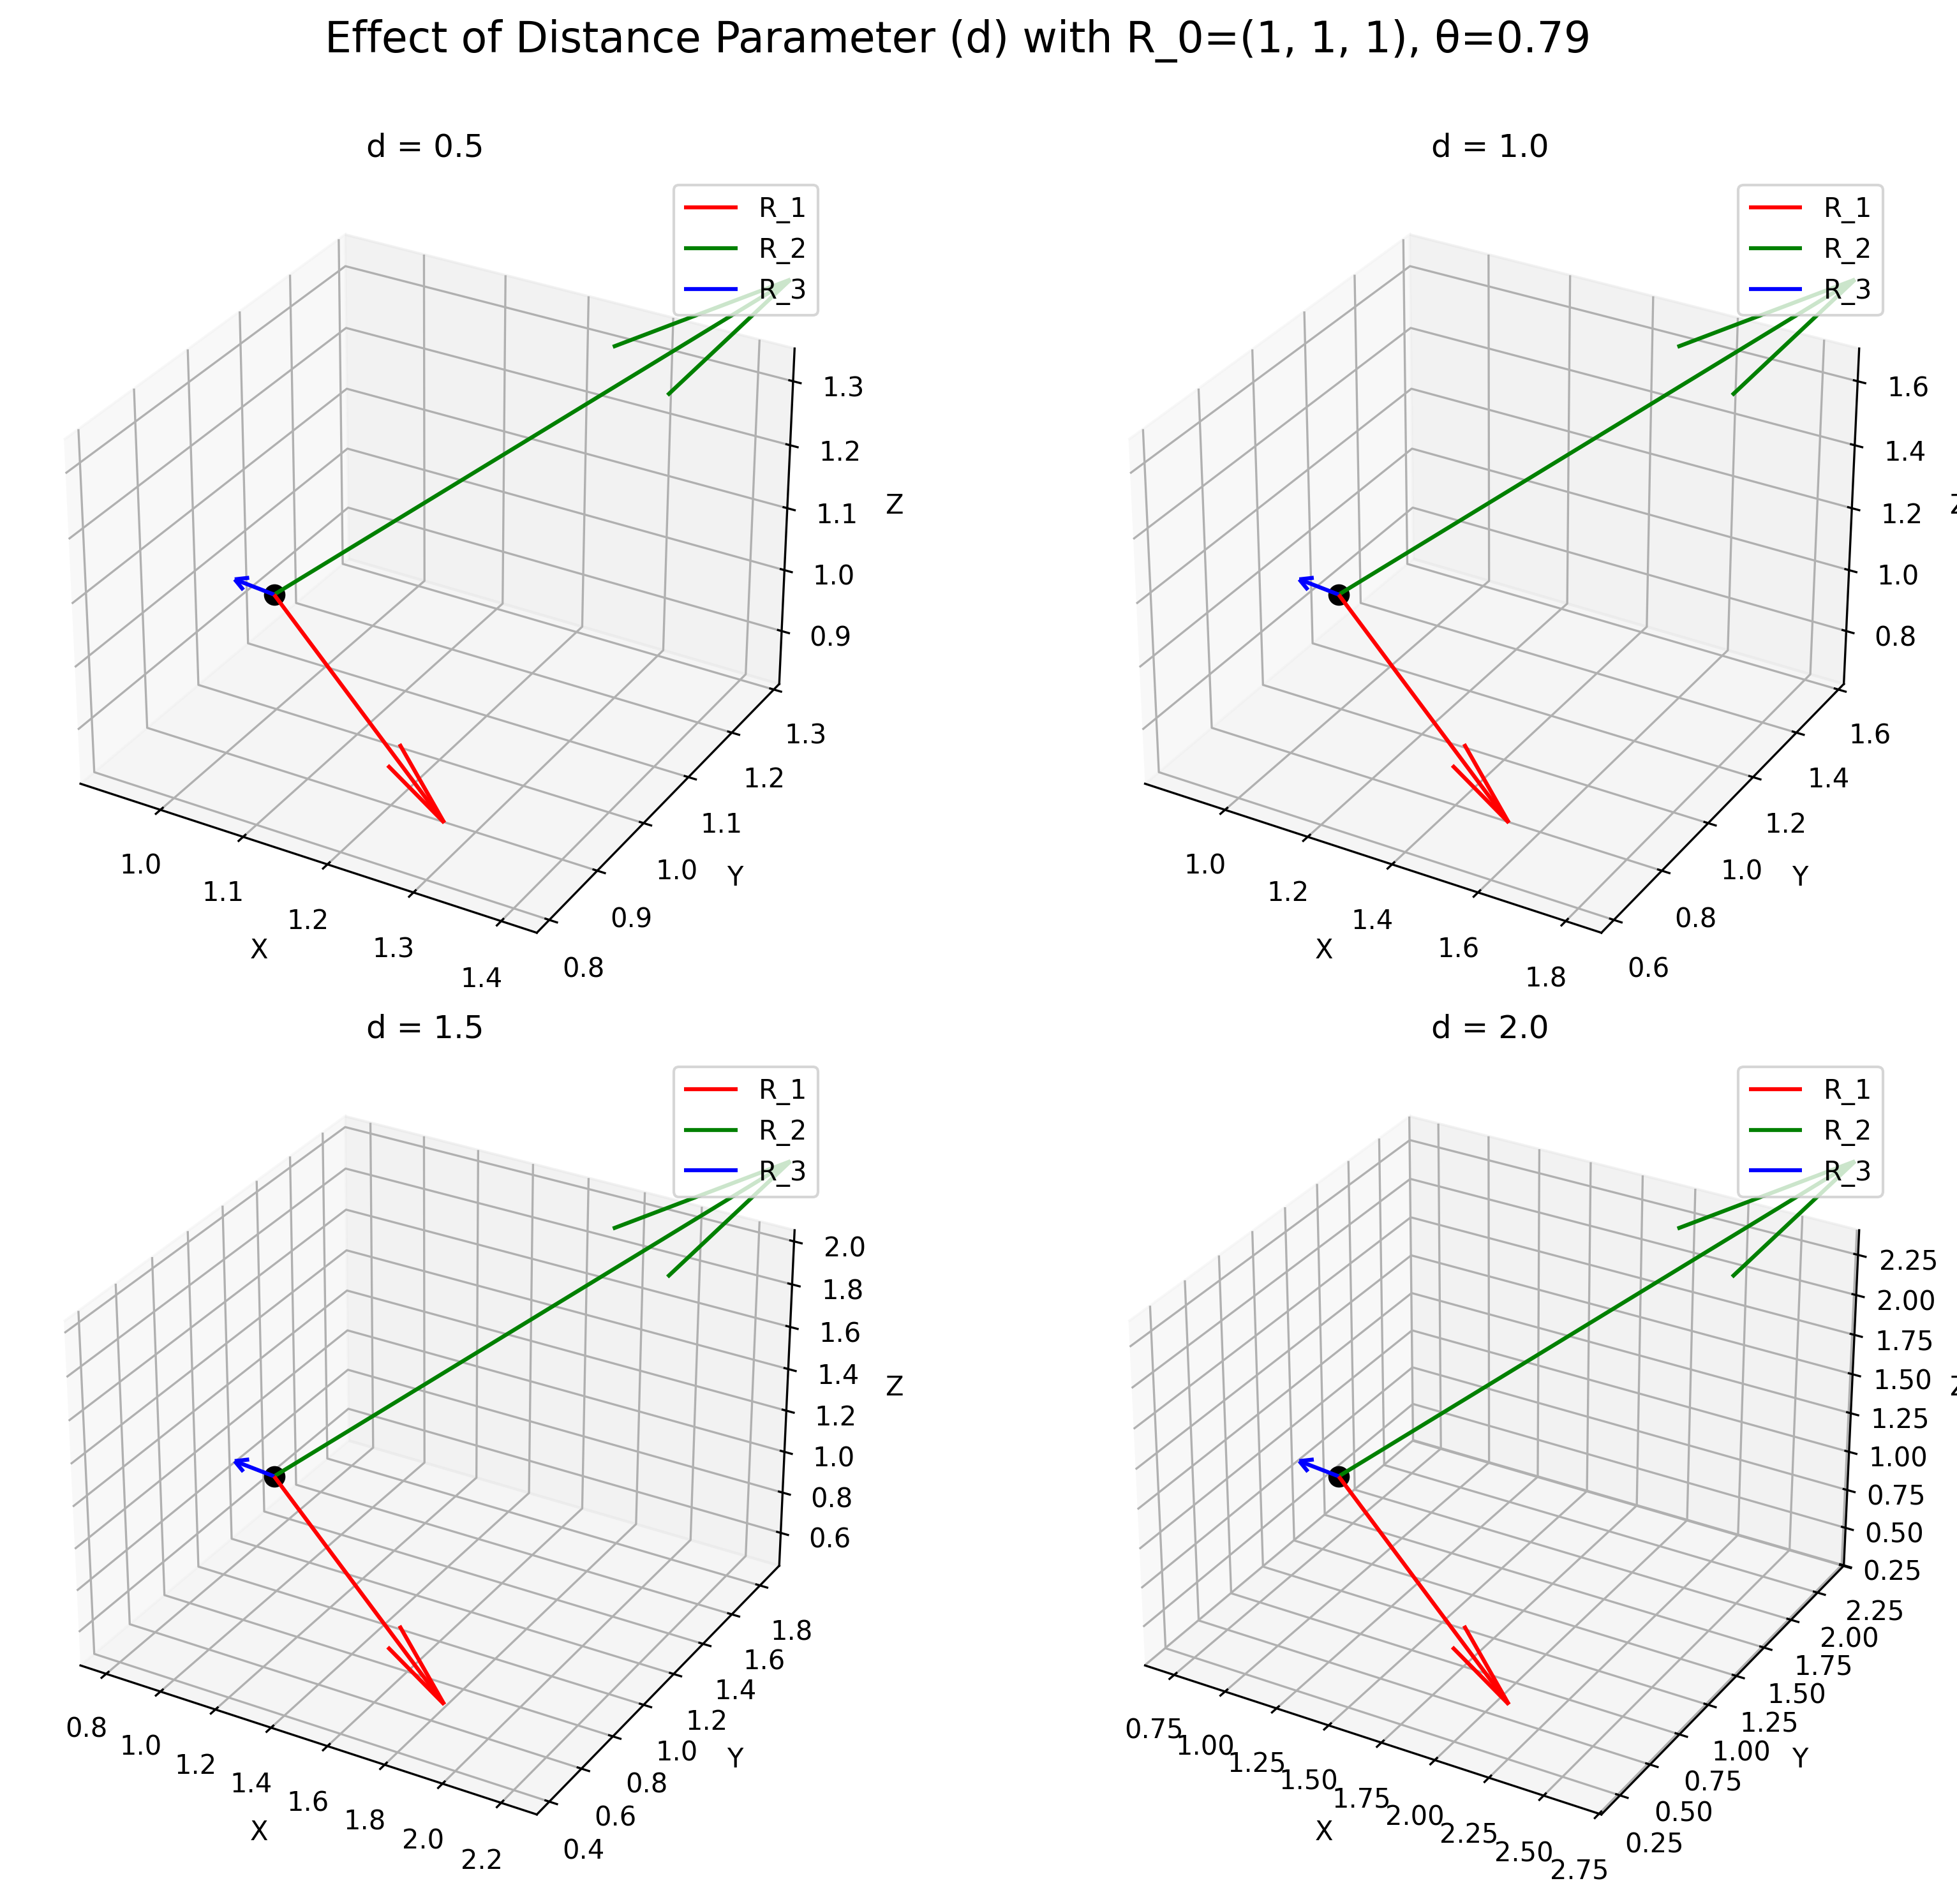
\includegraphics[width=0.9\textwidth]{figures/d_effect_R0_1_1_1.png}
    \caption{Effect of distance parameter on vector visualization with origin at $(1,1,1)$}
    \label{fig:example_distance_effect_custom1}
\end{figure}

\begin{figure}[H]
    \centering
    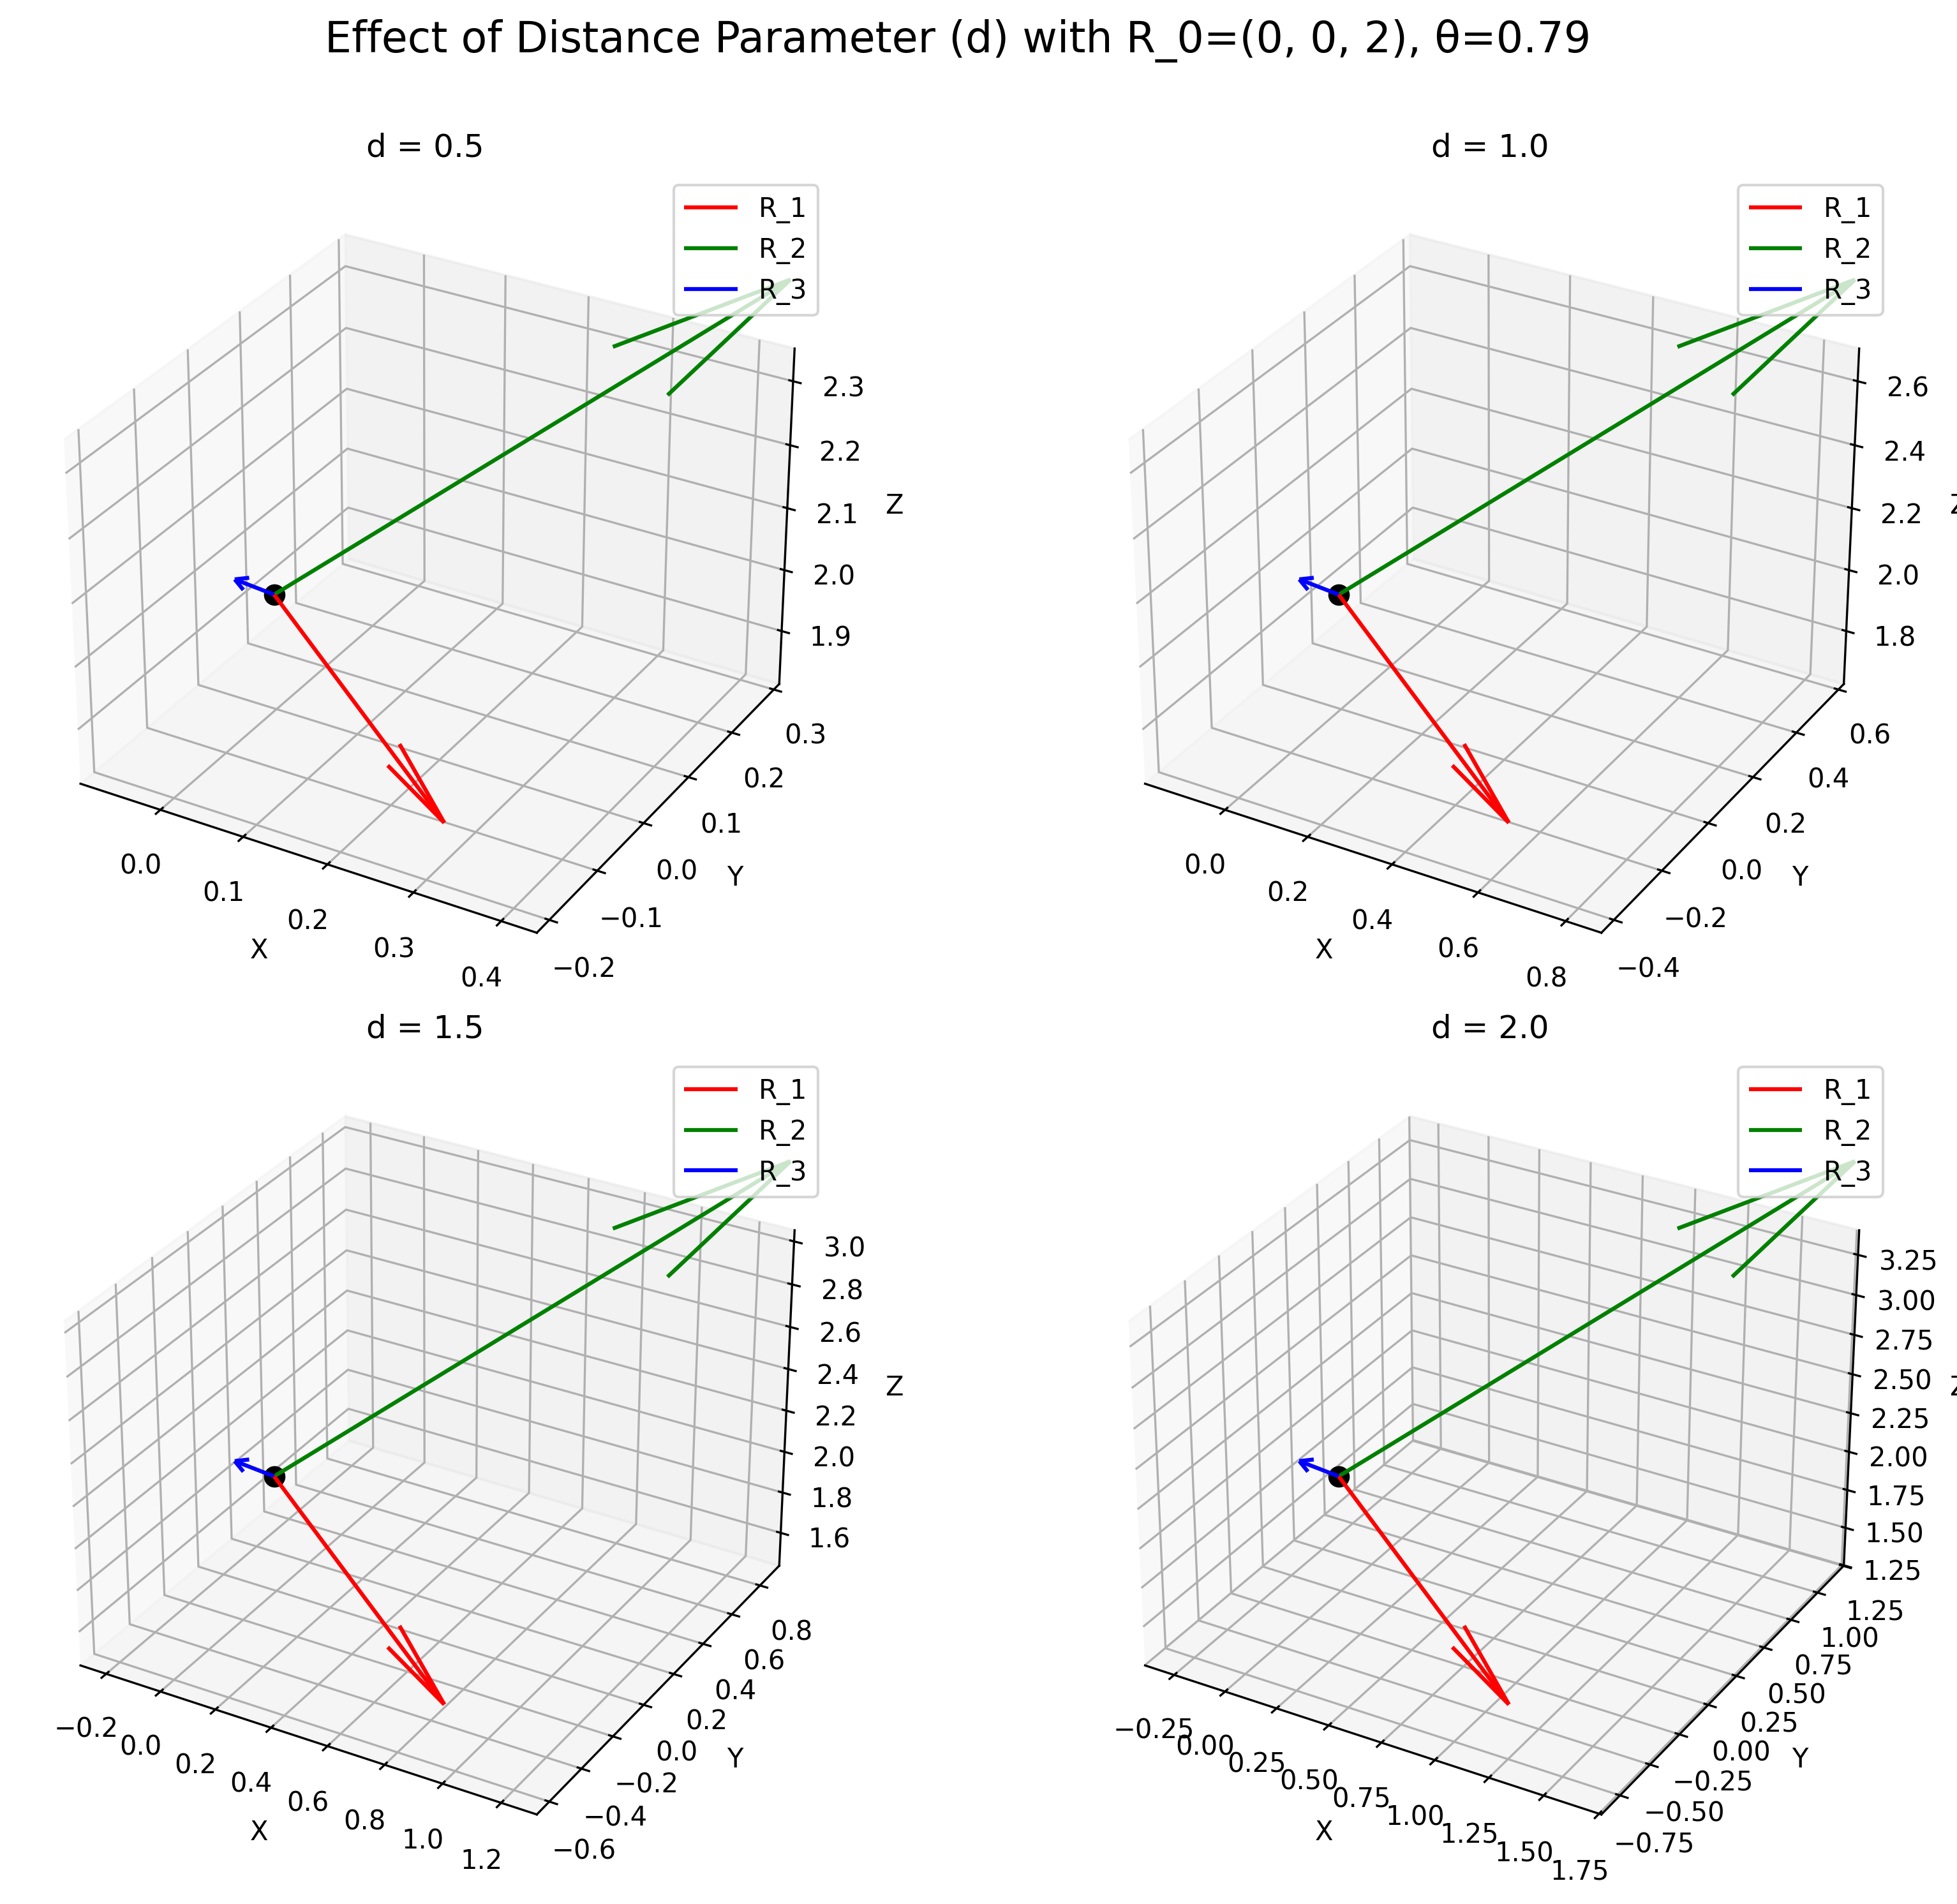
\includegraphics[width=0.9\textwidth]{figures/d_effect_R0_0_0_2.png}
    \caption{Effect of distance parameter on vector visualization with origin at $(0,0,2)$}
    \label{fig:example_distance_effect_custom2}
\end{figure}

\textbf{Effect of Distance Parameter:} The distance parameter $d$ scales the vectors equally, preserving their orthogonality. Increasing $d$ increases the distance of the vectors from the origin, while decreasing $d$ decreases the distance. As shown in the figures above, the effect is consistent across different origin points.

\subsection{Effect of Angle Parameter}

The angle parameter $\theta$ rotates the vectors around the origin, preserving their orthogonality. Different values of $\theta$ result in different orientations of the vectors.

\begin{figure}[H]
    \centering
    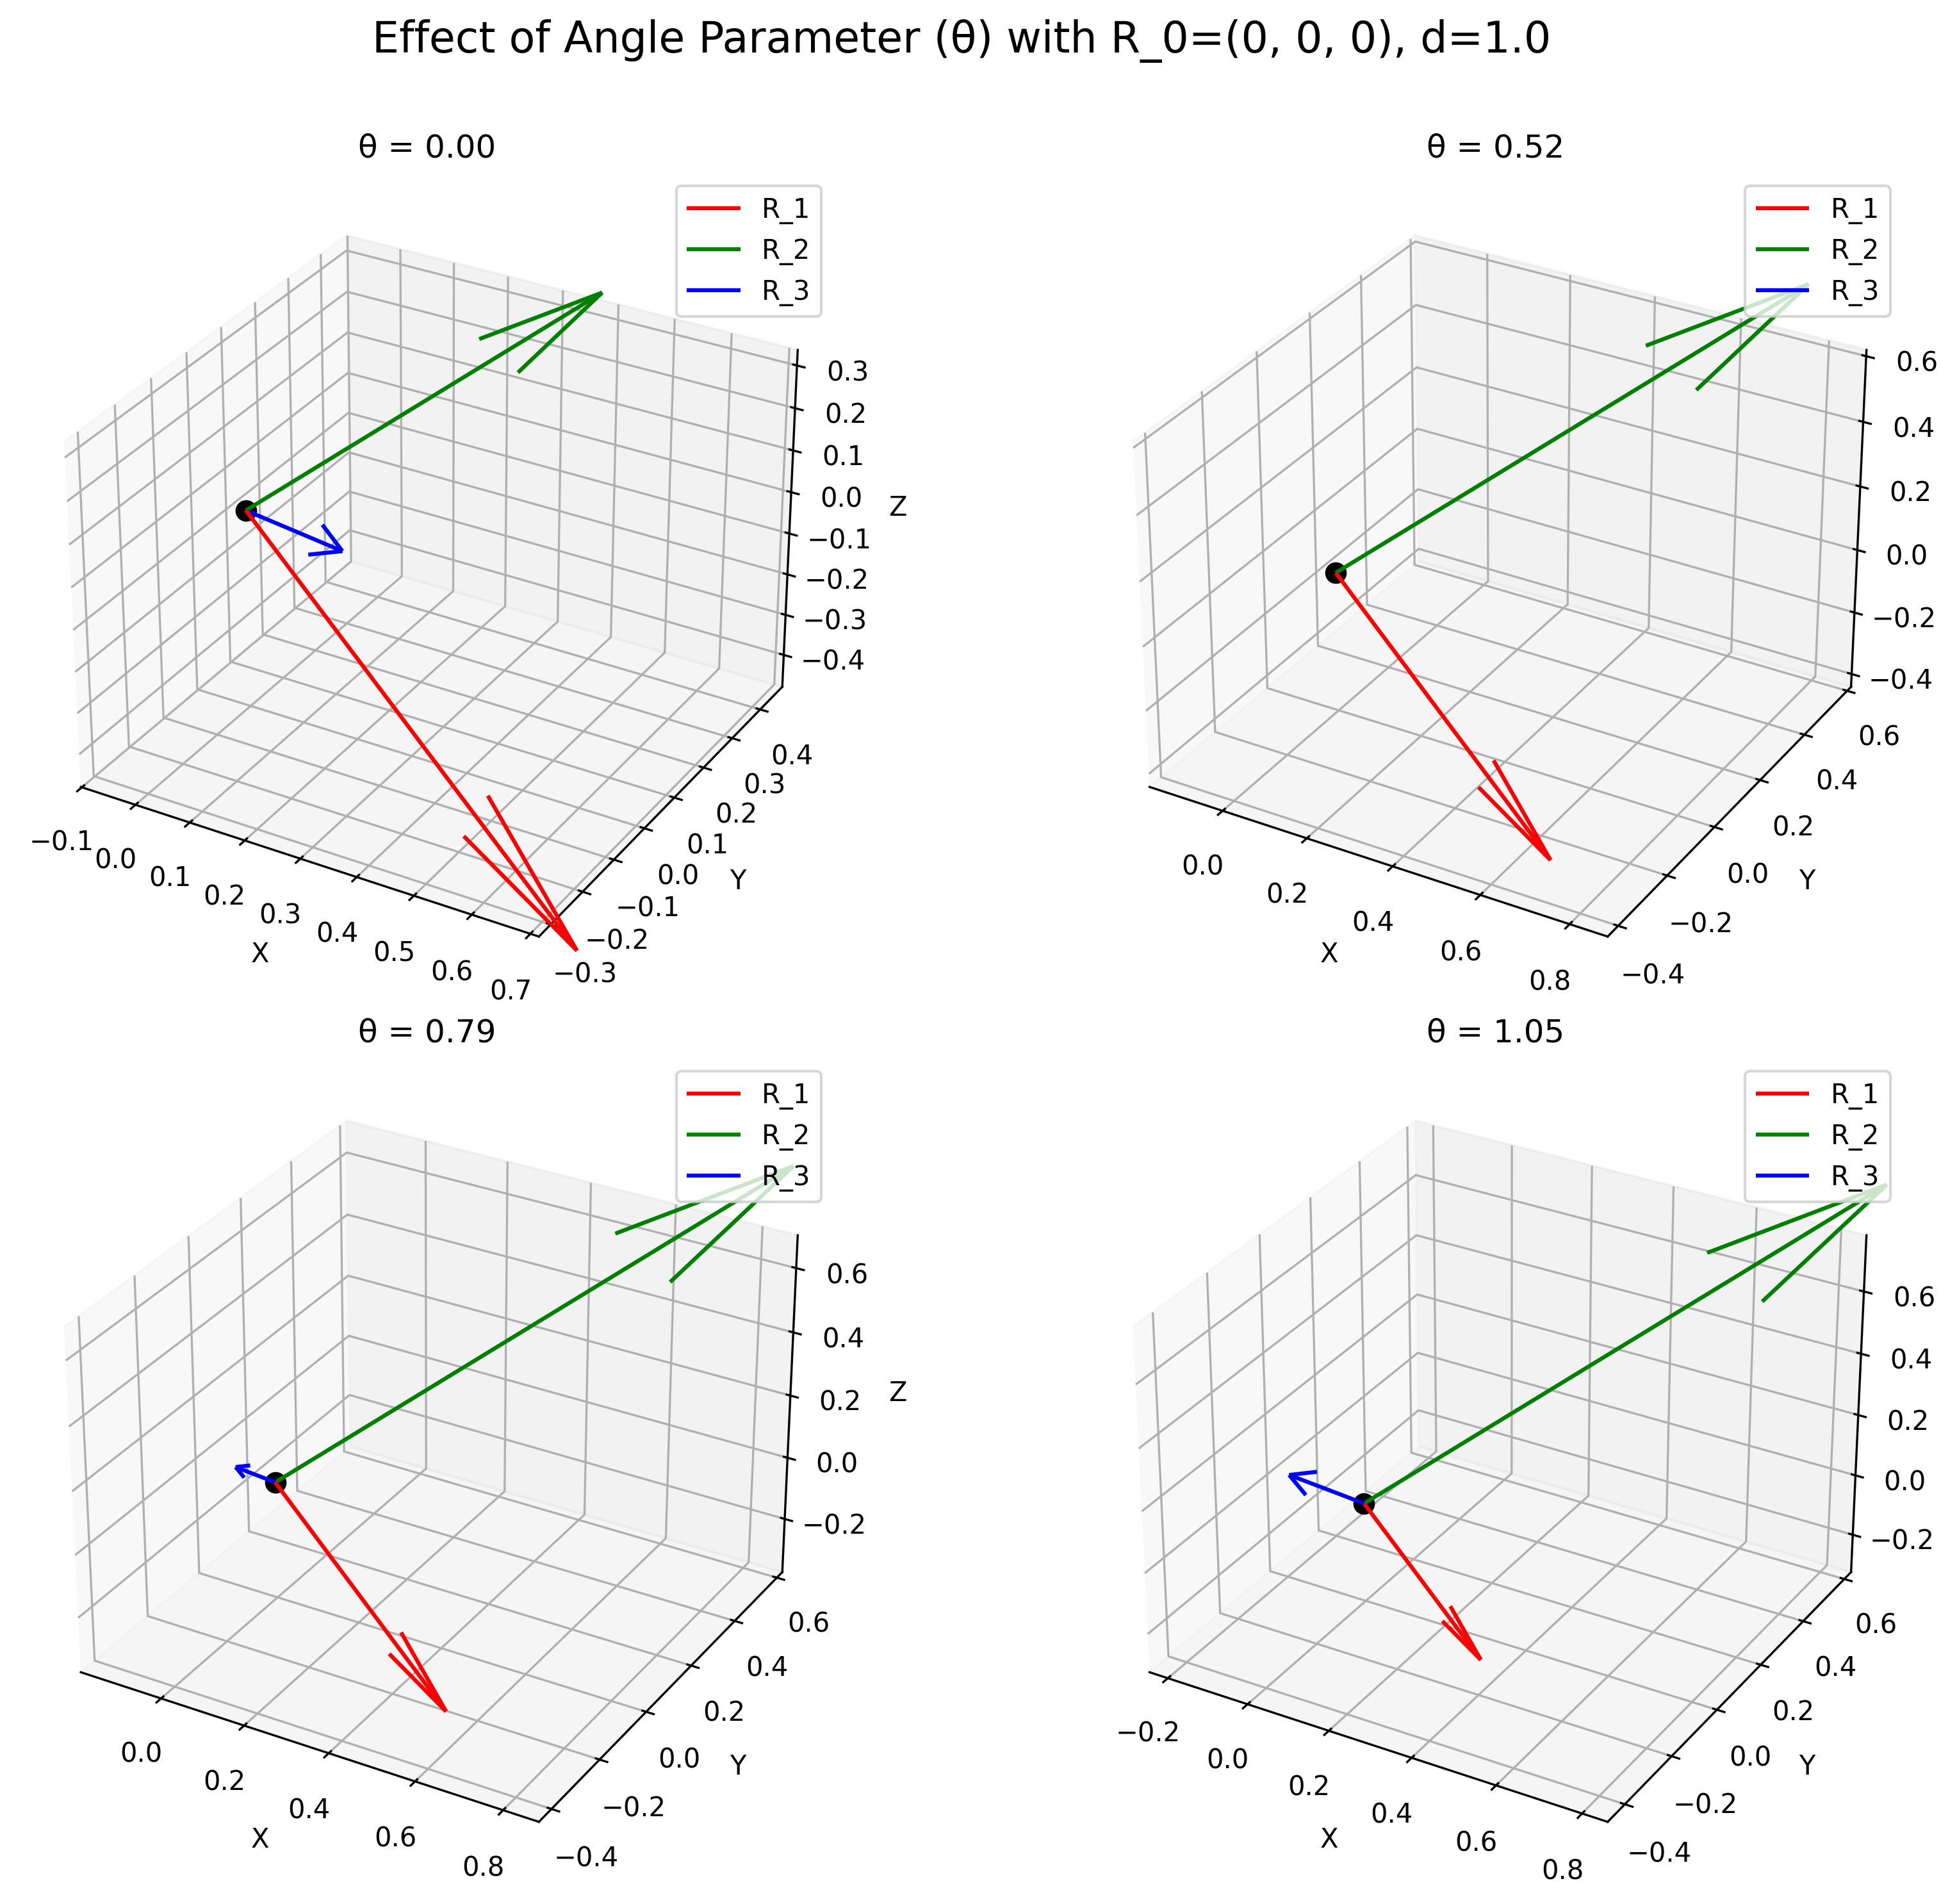
\includegraphics[width=0.9\textwidth]{figures/theta_effect_R0_0_0_0.png}
    \caption{Effect of angle parameter on vector visualization with origin at $(0,0,0)$}
    \label{fig:example_angle_effect_default}
\end{figure}

\begin{figure}[H]
    \centering
    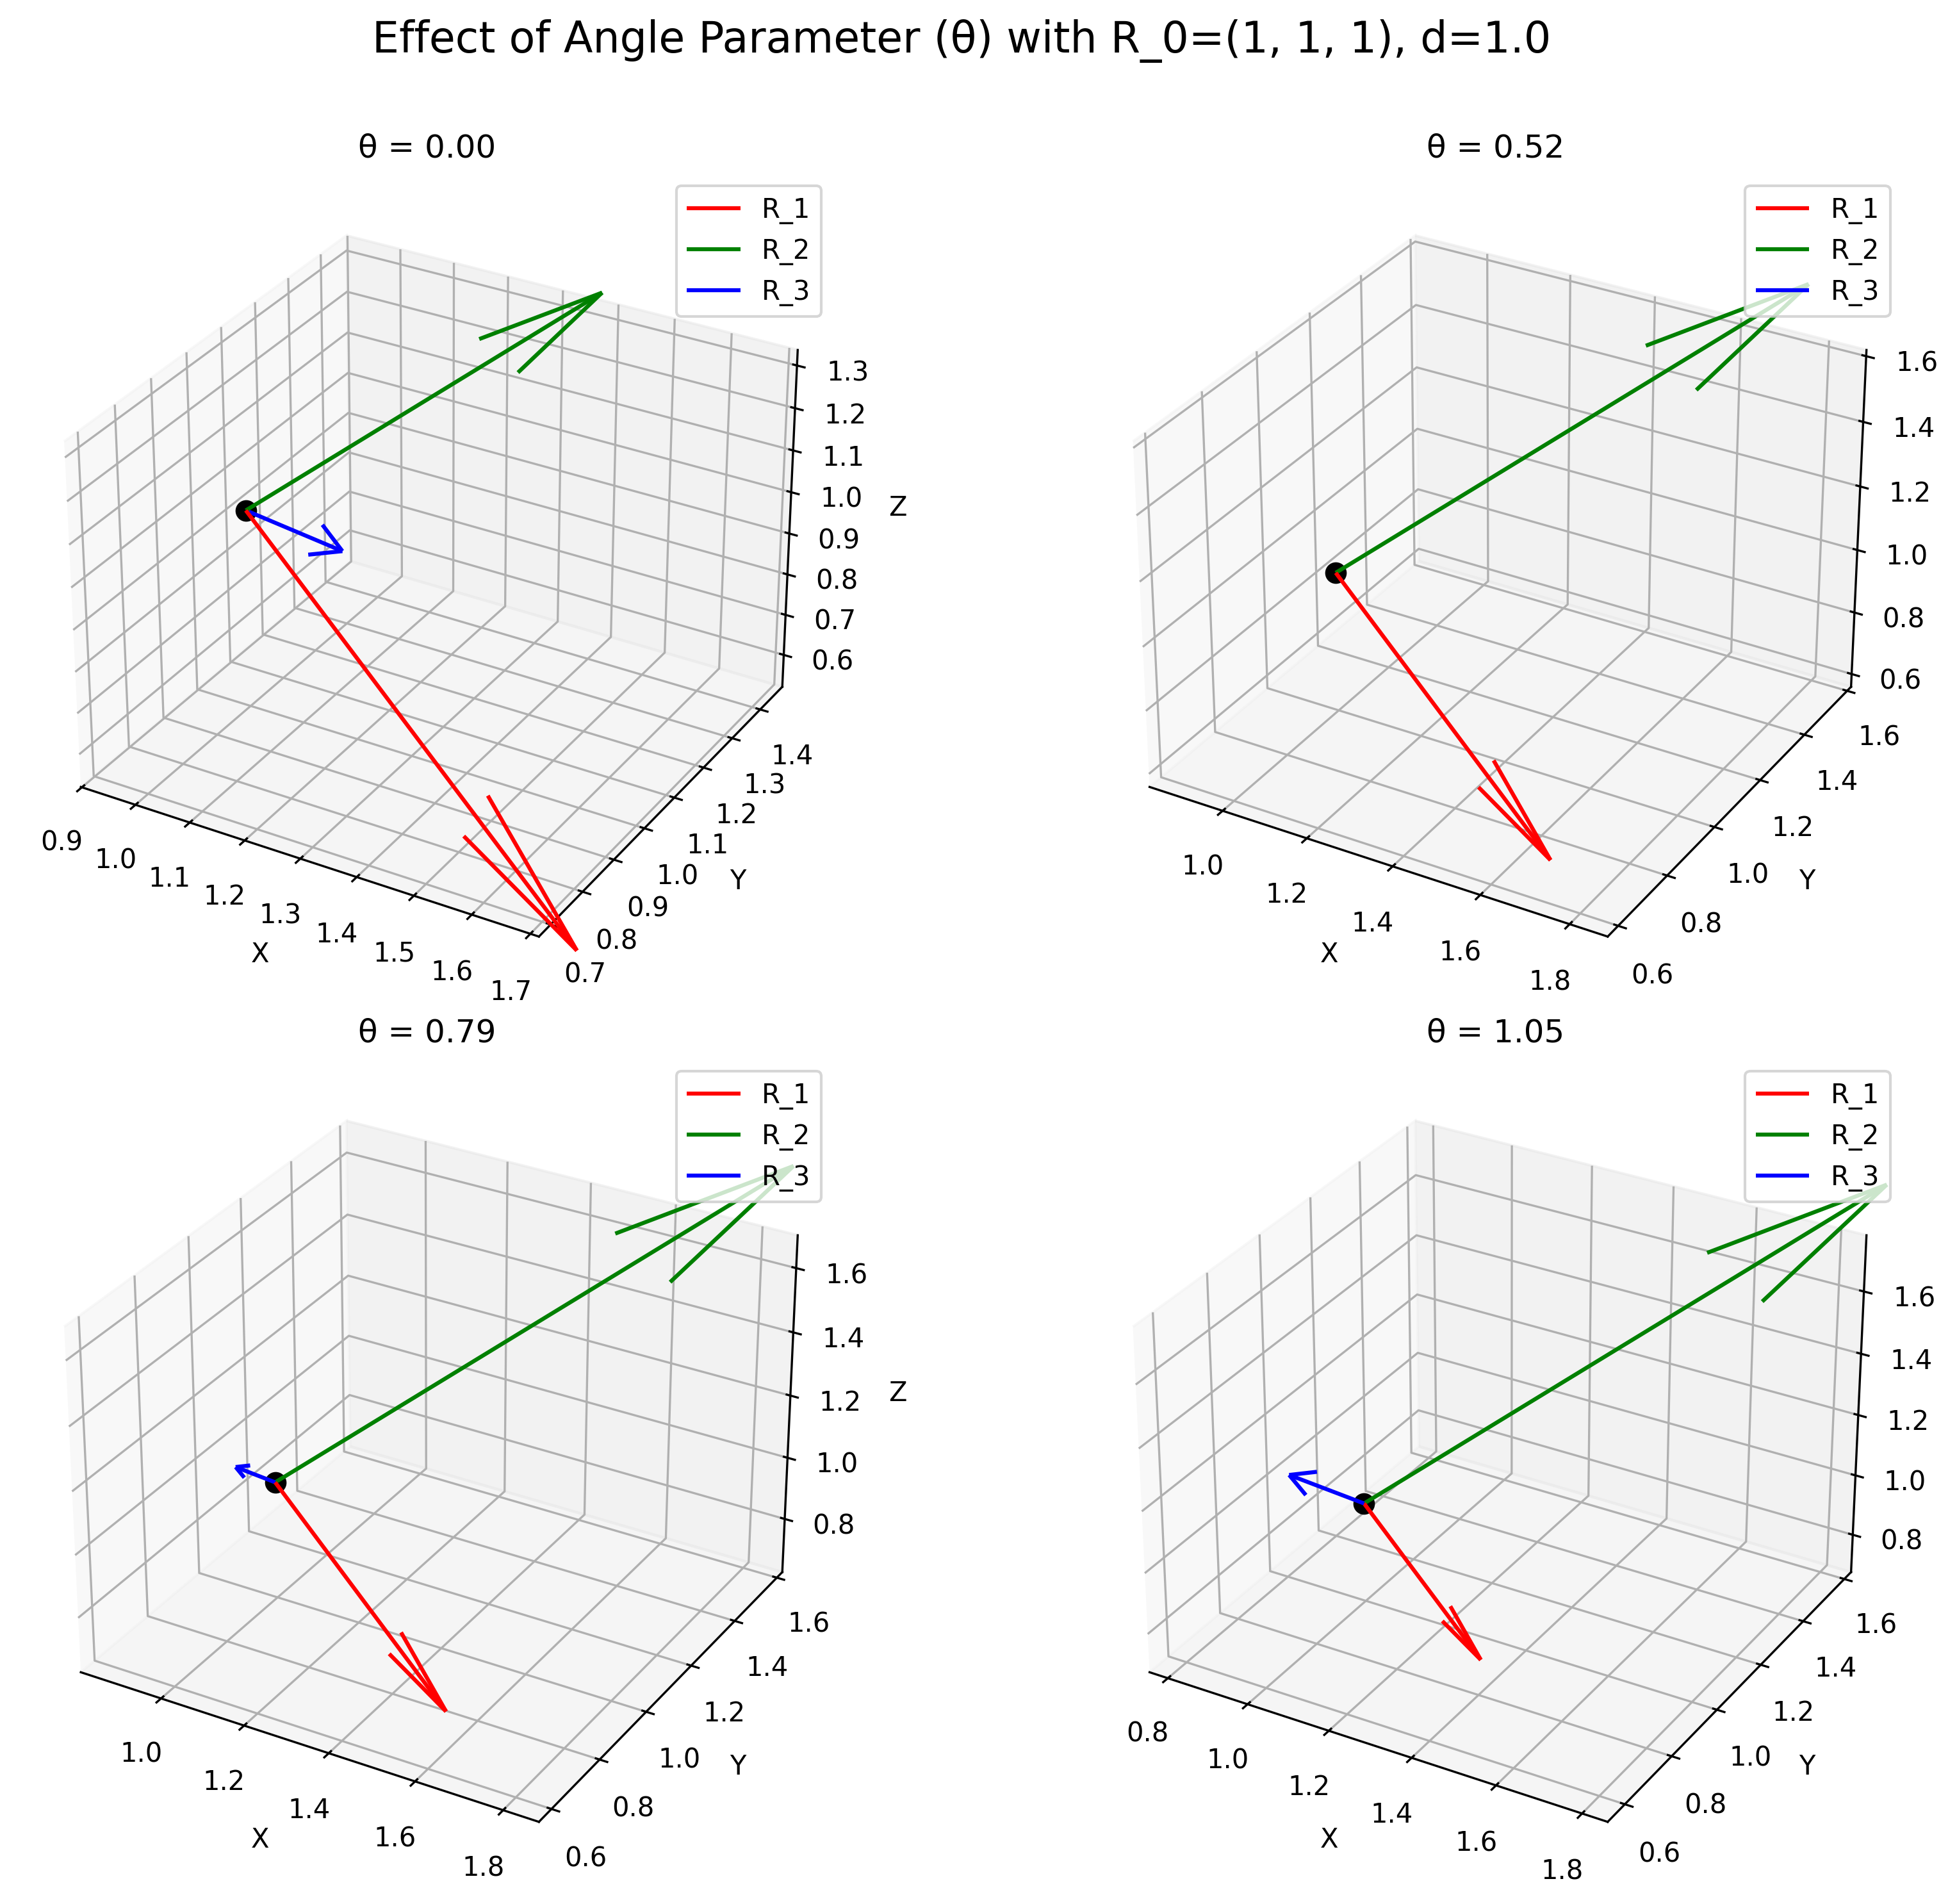
\includegraphics[width=0.9\textwidth]{figures/theta_effect_R0_1_1_1.png}
    \caption{Effect of angle parameter on vector visualization with origin at $(1,1,1)$}
    \label{fig:example_angle_effect_custom1}
\end{figure}

\begin{figure}[H]
    \centering
    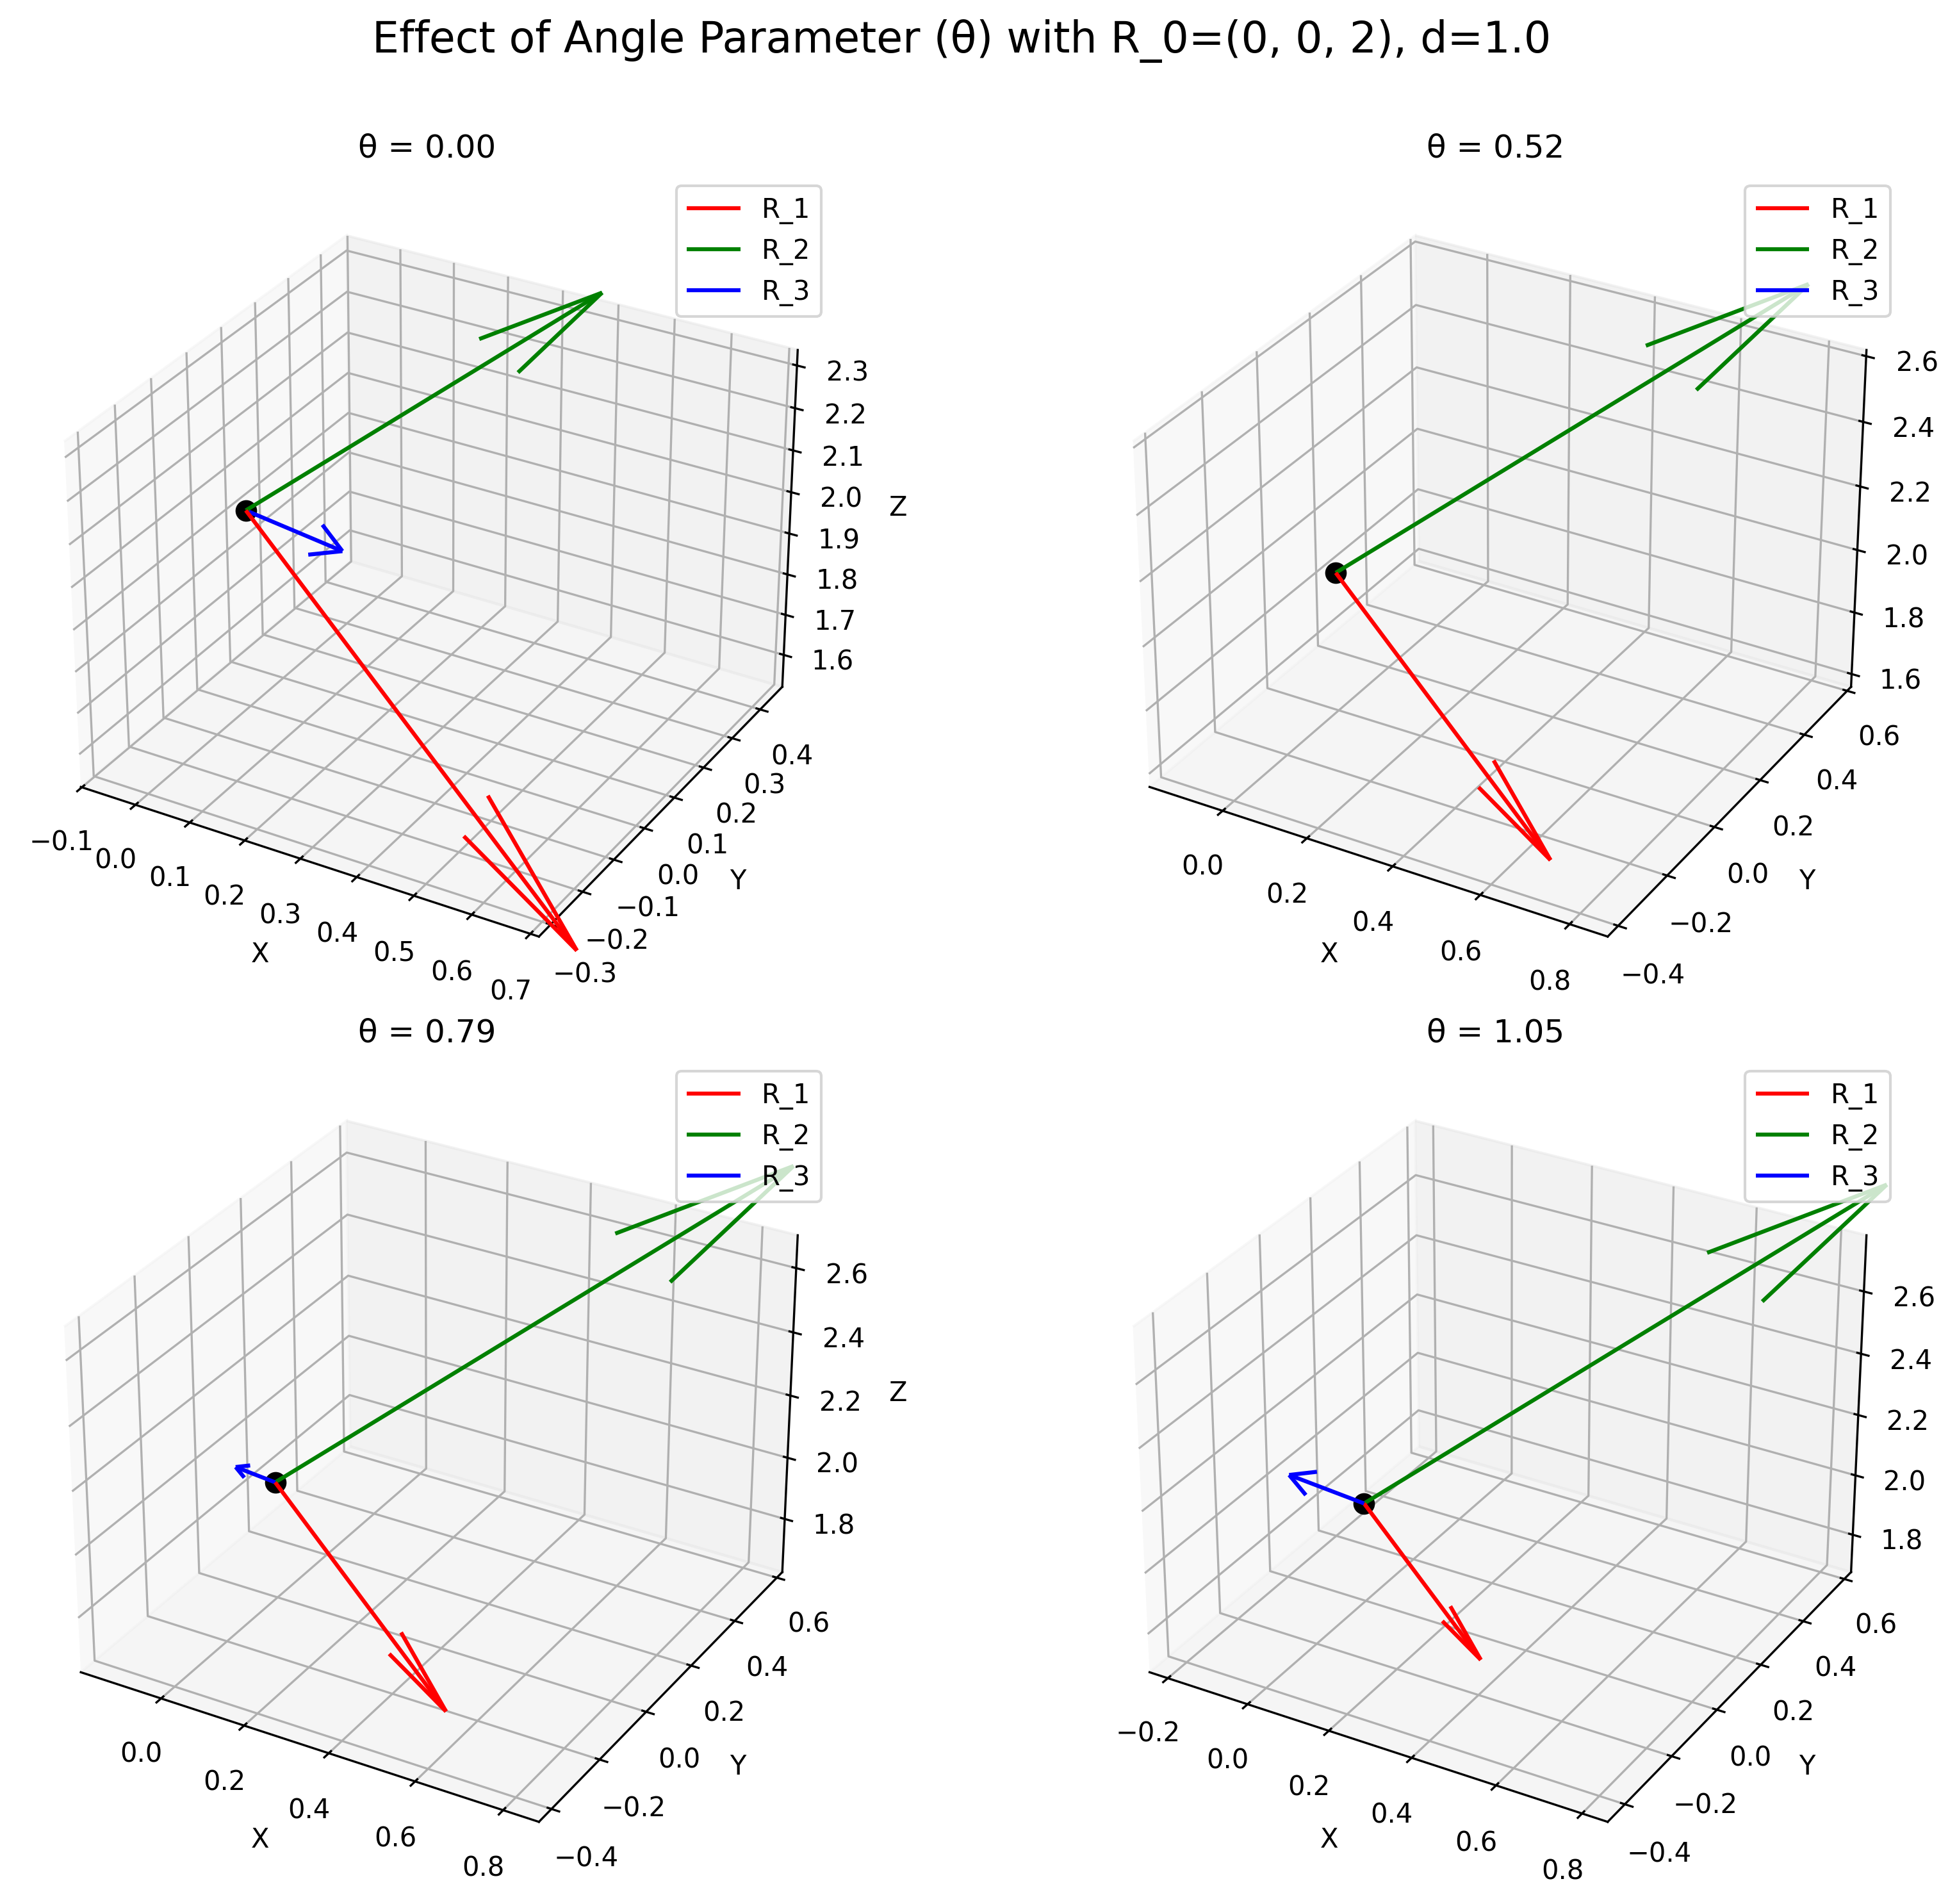
\includegraphics[width=0.9\textwidth]{figures/theta_effect_R0_0_0_2.png}
    \caption{Effect of angle parameter on vector visualization with origin at $(0,0,2)$}
    \label{fig:example_angle_effect_custom2}
\end{figure}

\textbf{Effect of Angle Parameter:} The angle parameter $\theta$ rotates the vectors around the origin, preserving their orthogonality. Different values of $\theta$ result in different orientations of the vectors. As shown in the figures above, the effect is consistent across different origin points, with the rotation occurring relative to the specified origin.

\subsection{Effect of Origin}

The origin parameter $\vec{R}_0$ shifts the entire vector system, preserving the orthogonality of the displacement vectors. Different origin points result in different positions of the vectors in space.

\subsubsection{3D Visualizations}

\begin{figure}[H]
    \centering
    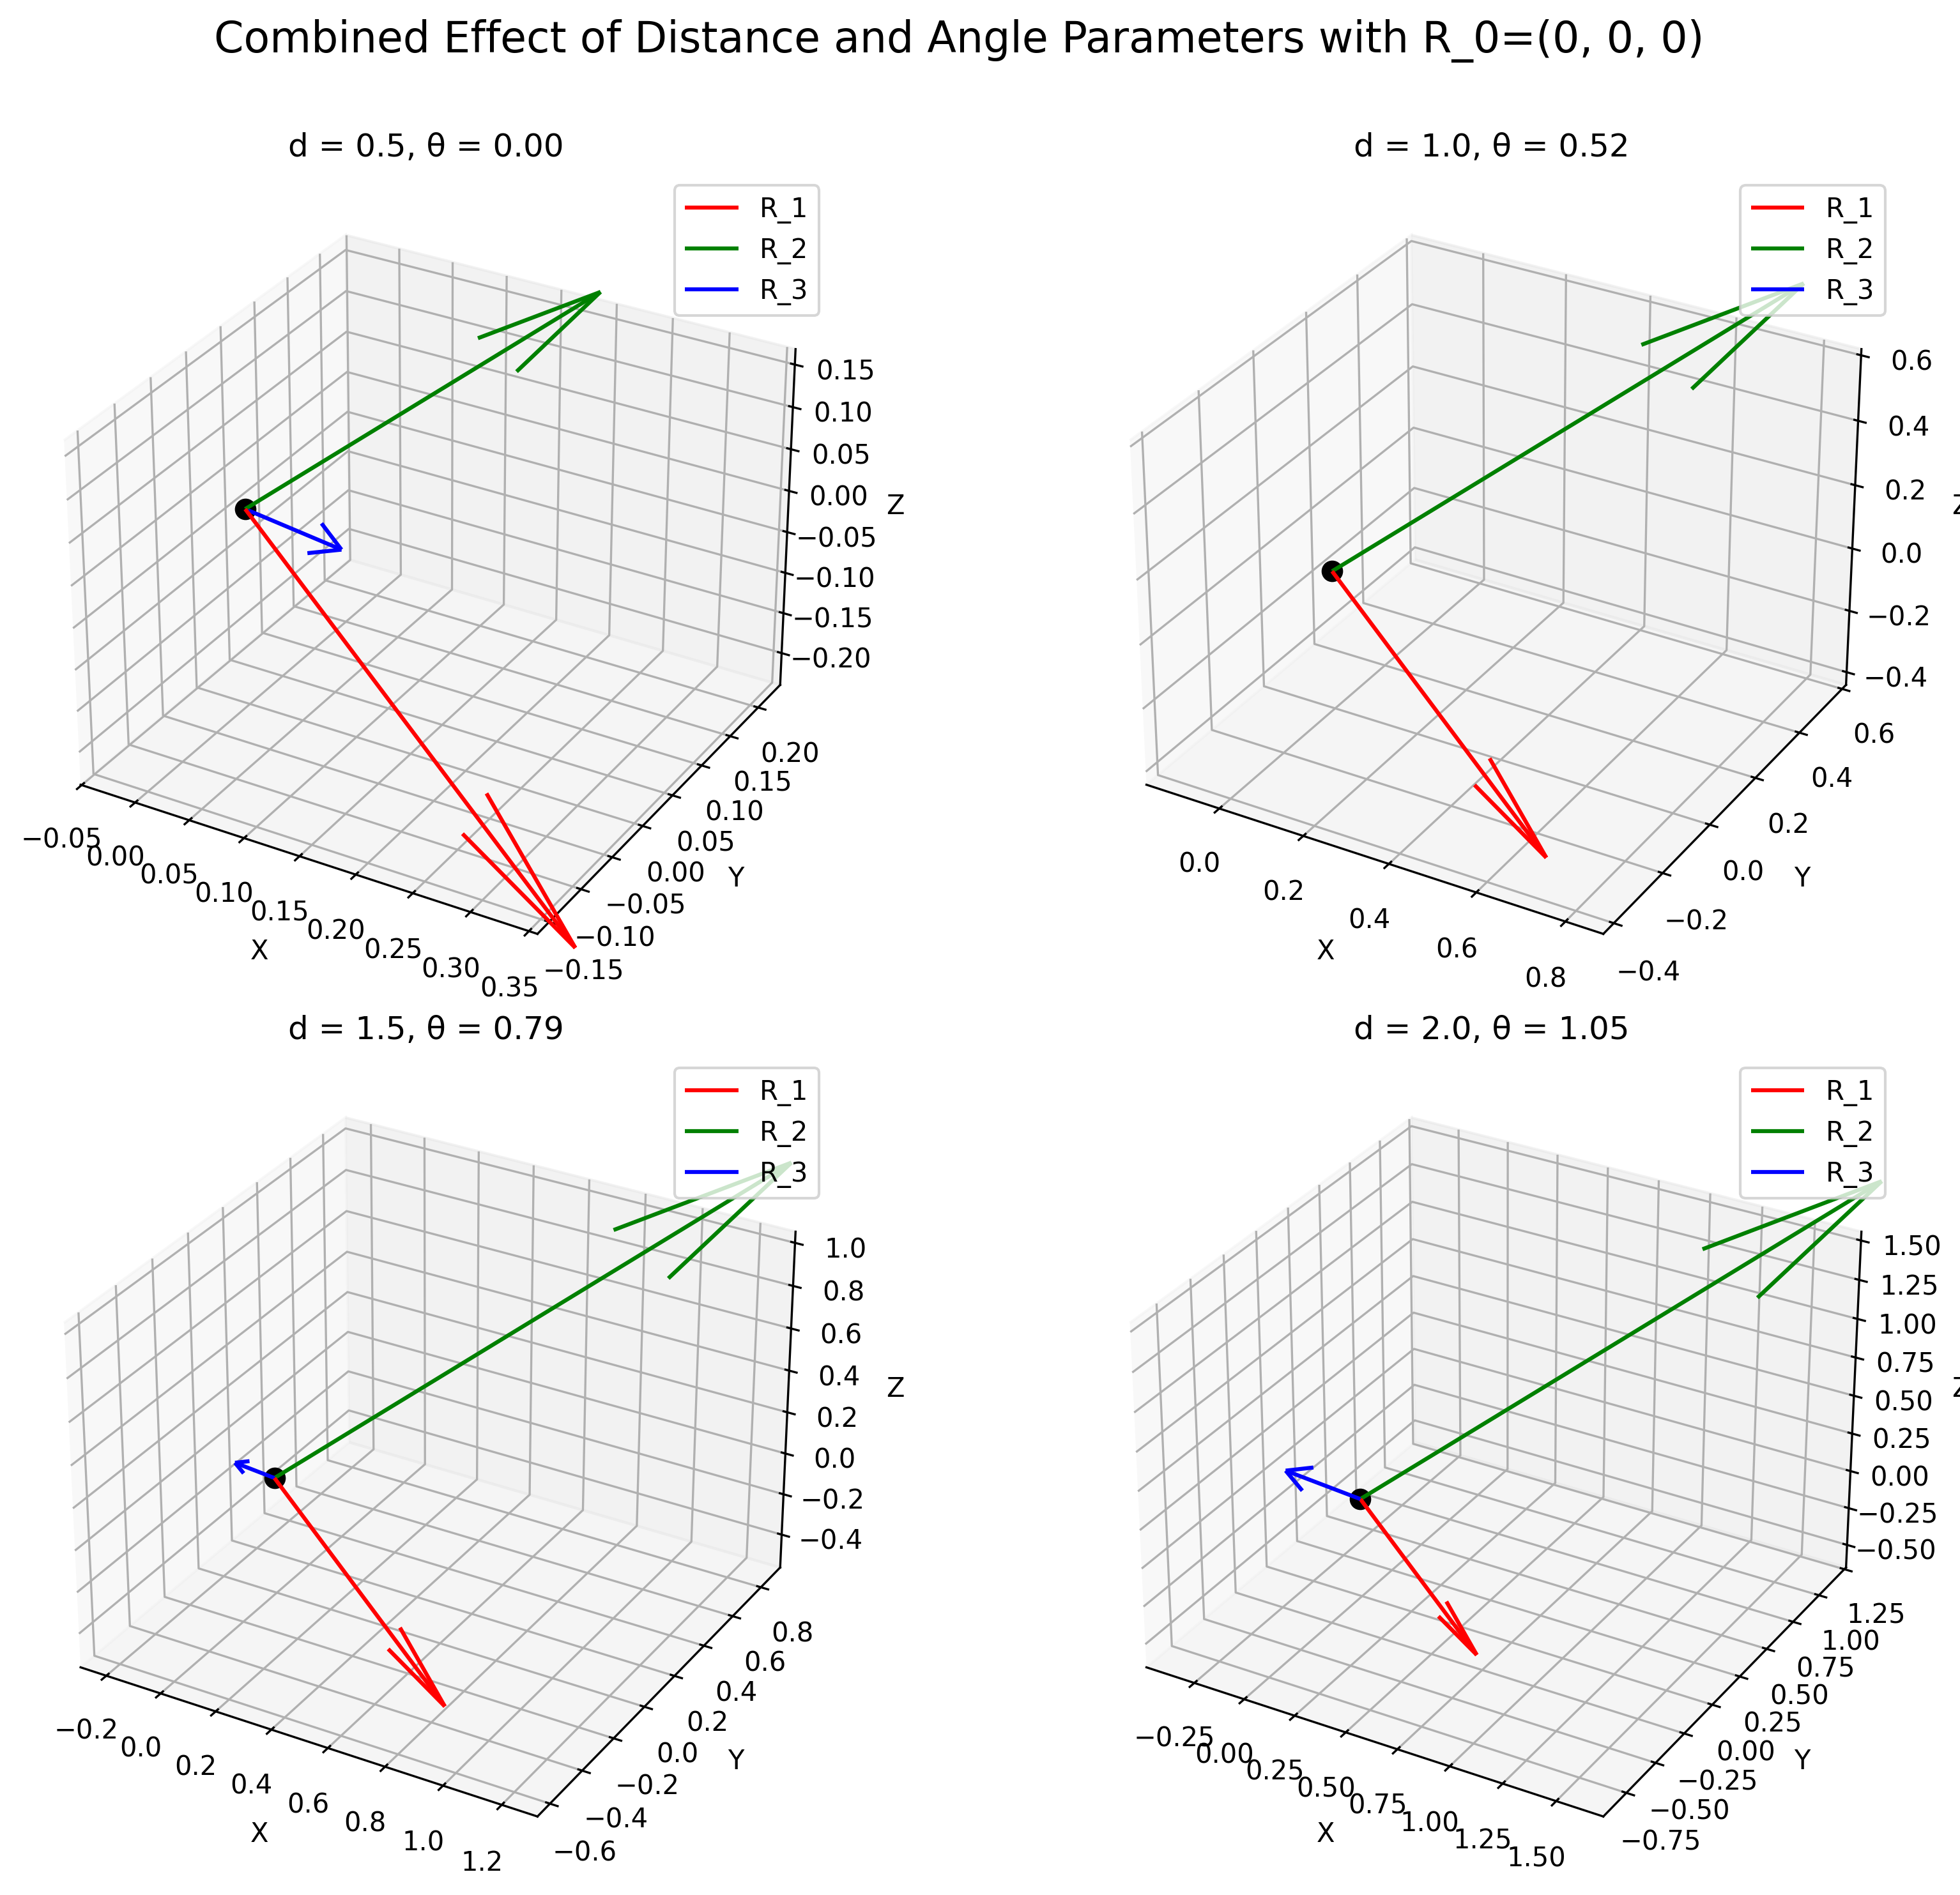
\includegraphics[width=0.9\textwidth]{figures/combined_effect_R0_0_0_0.png}
    \caption{Combined effect of distance and angle parameters with origin at $(0,0,0)$}
    \label{fig:example_combined_effect_default}
\end{figure}

\begin{figure}[H]
    \centering
    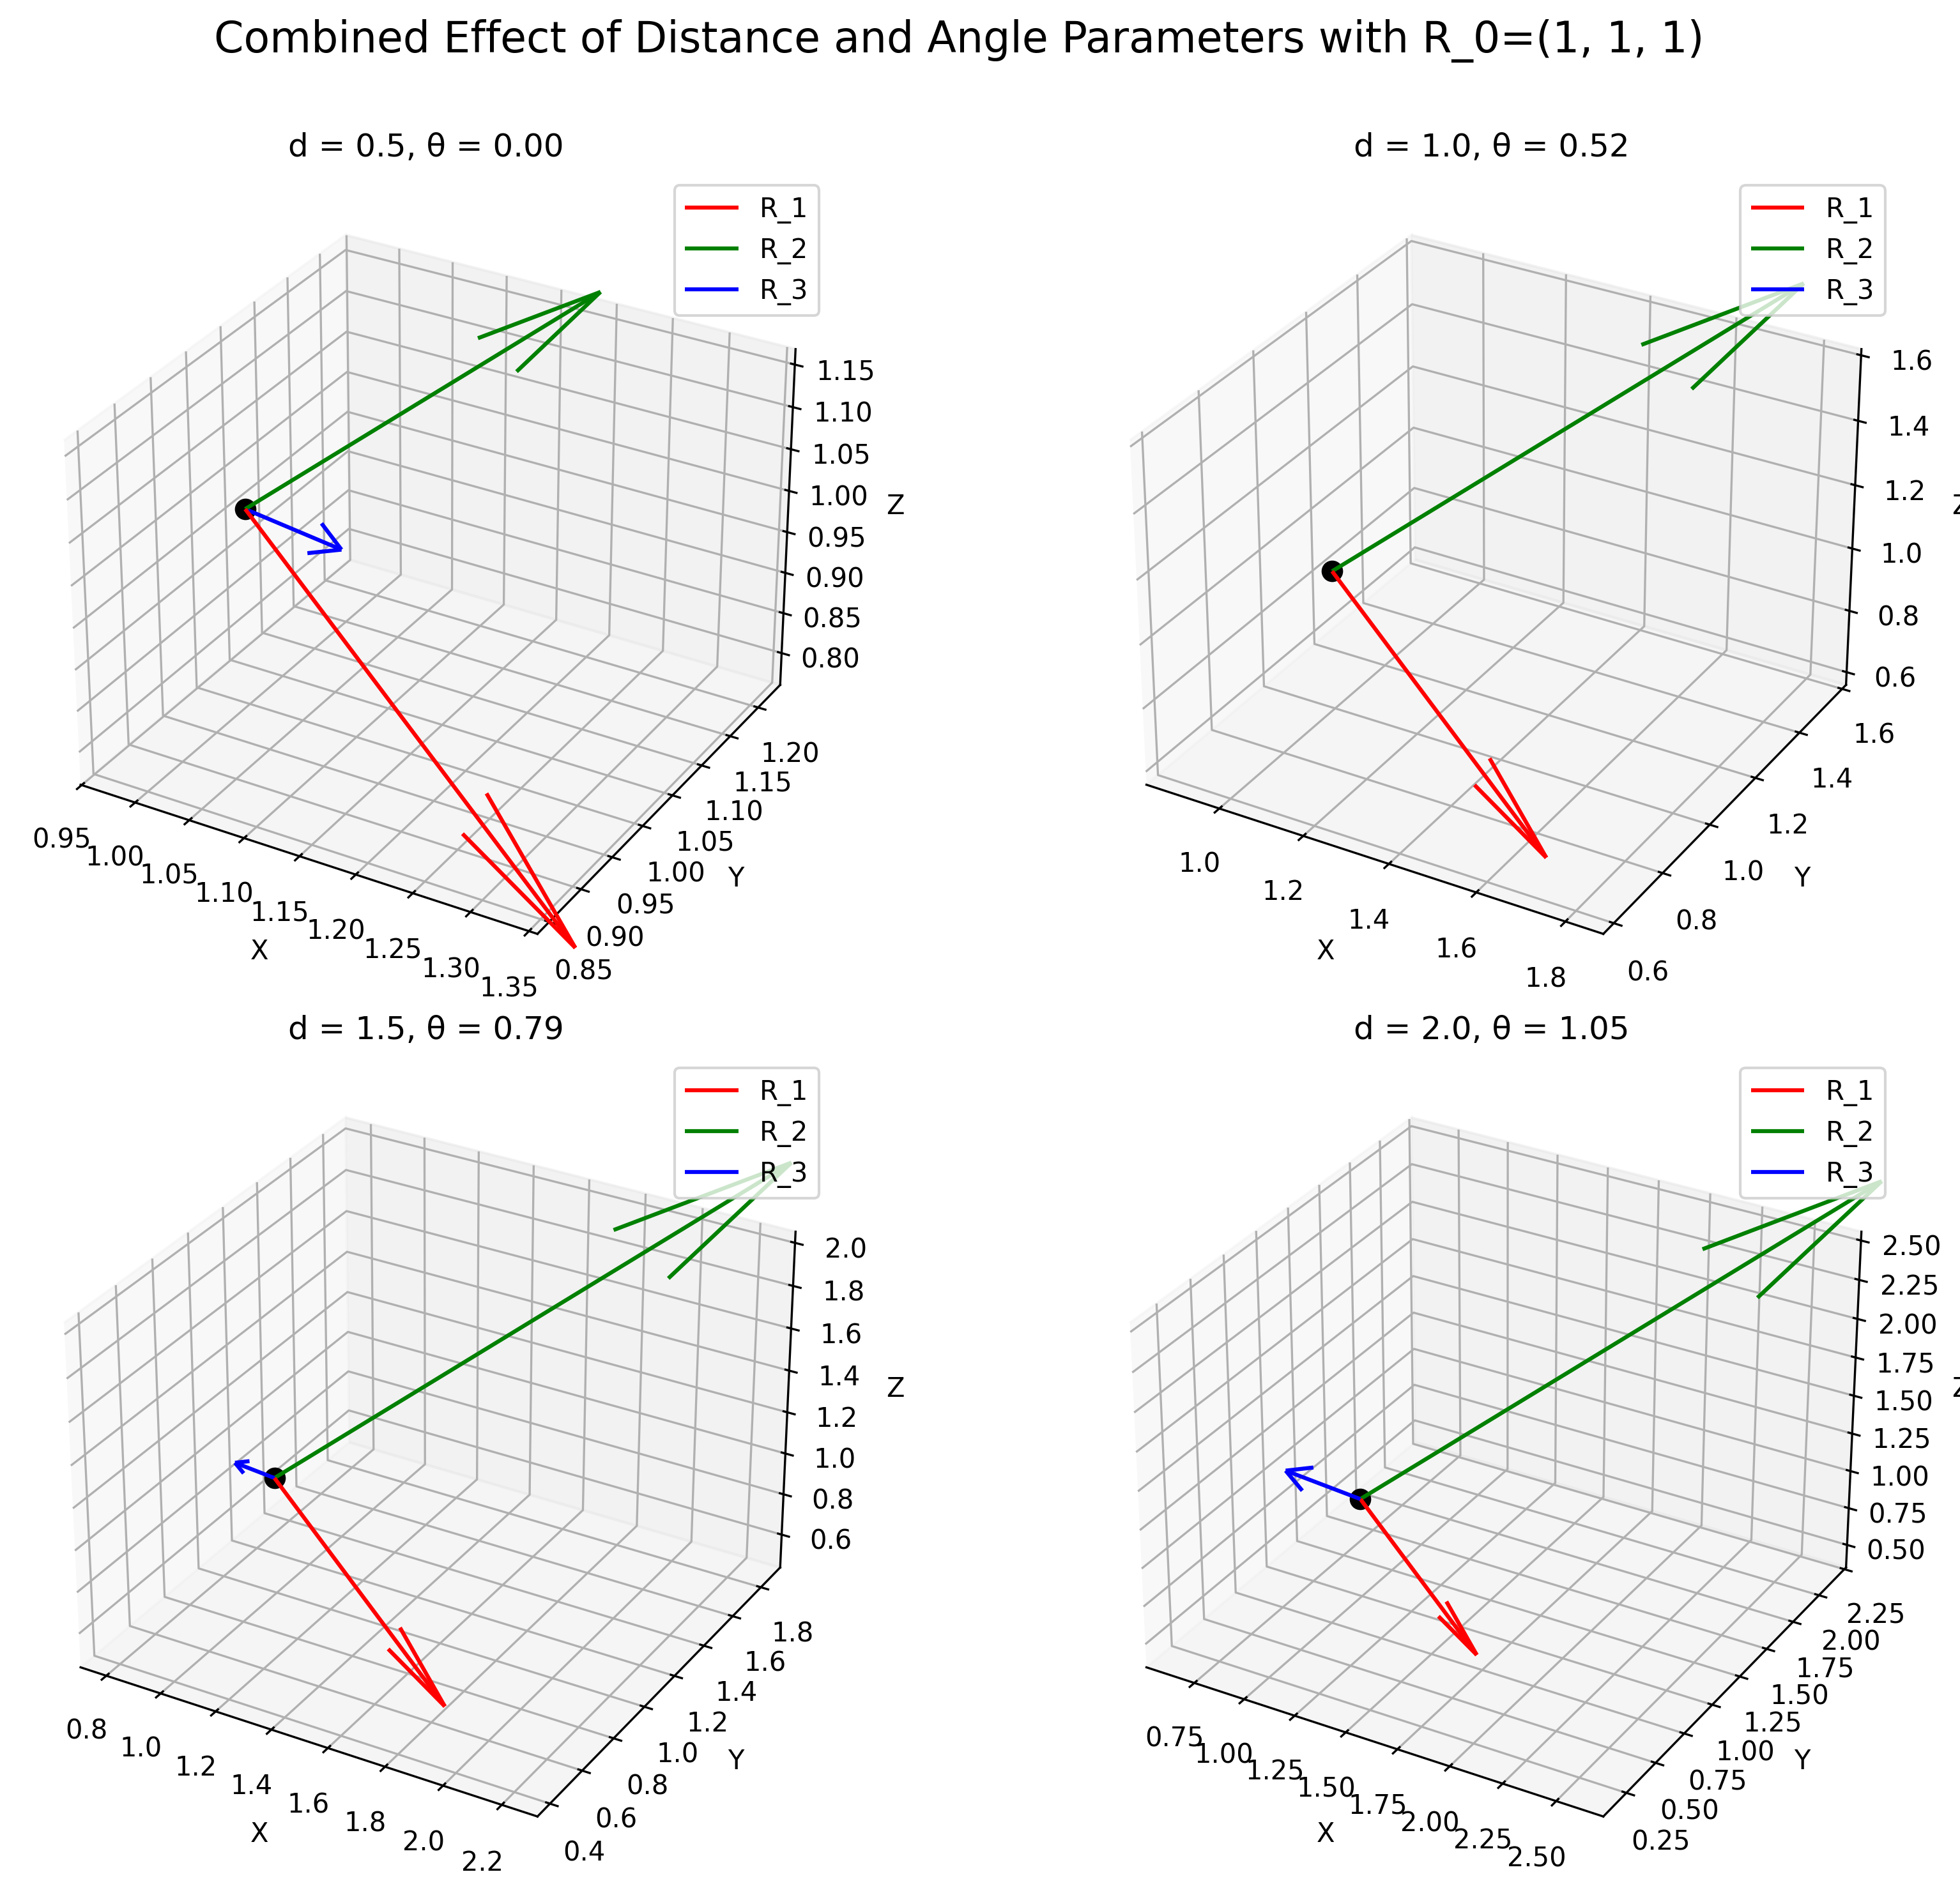
\includegraphics[width=0.9\textwidth]{figures/combined_effect_R0_1_1_1.png}
    \caption{Combined effect of distance and angle parameters with origin at $(1,1,1)$}
    \label{fig:example_combined_effect_custom1}
\end{figure}

\begin{figure}[H]
    \centering
    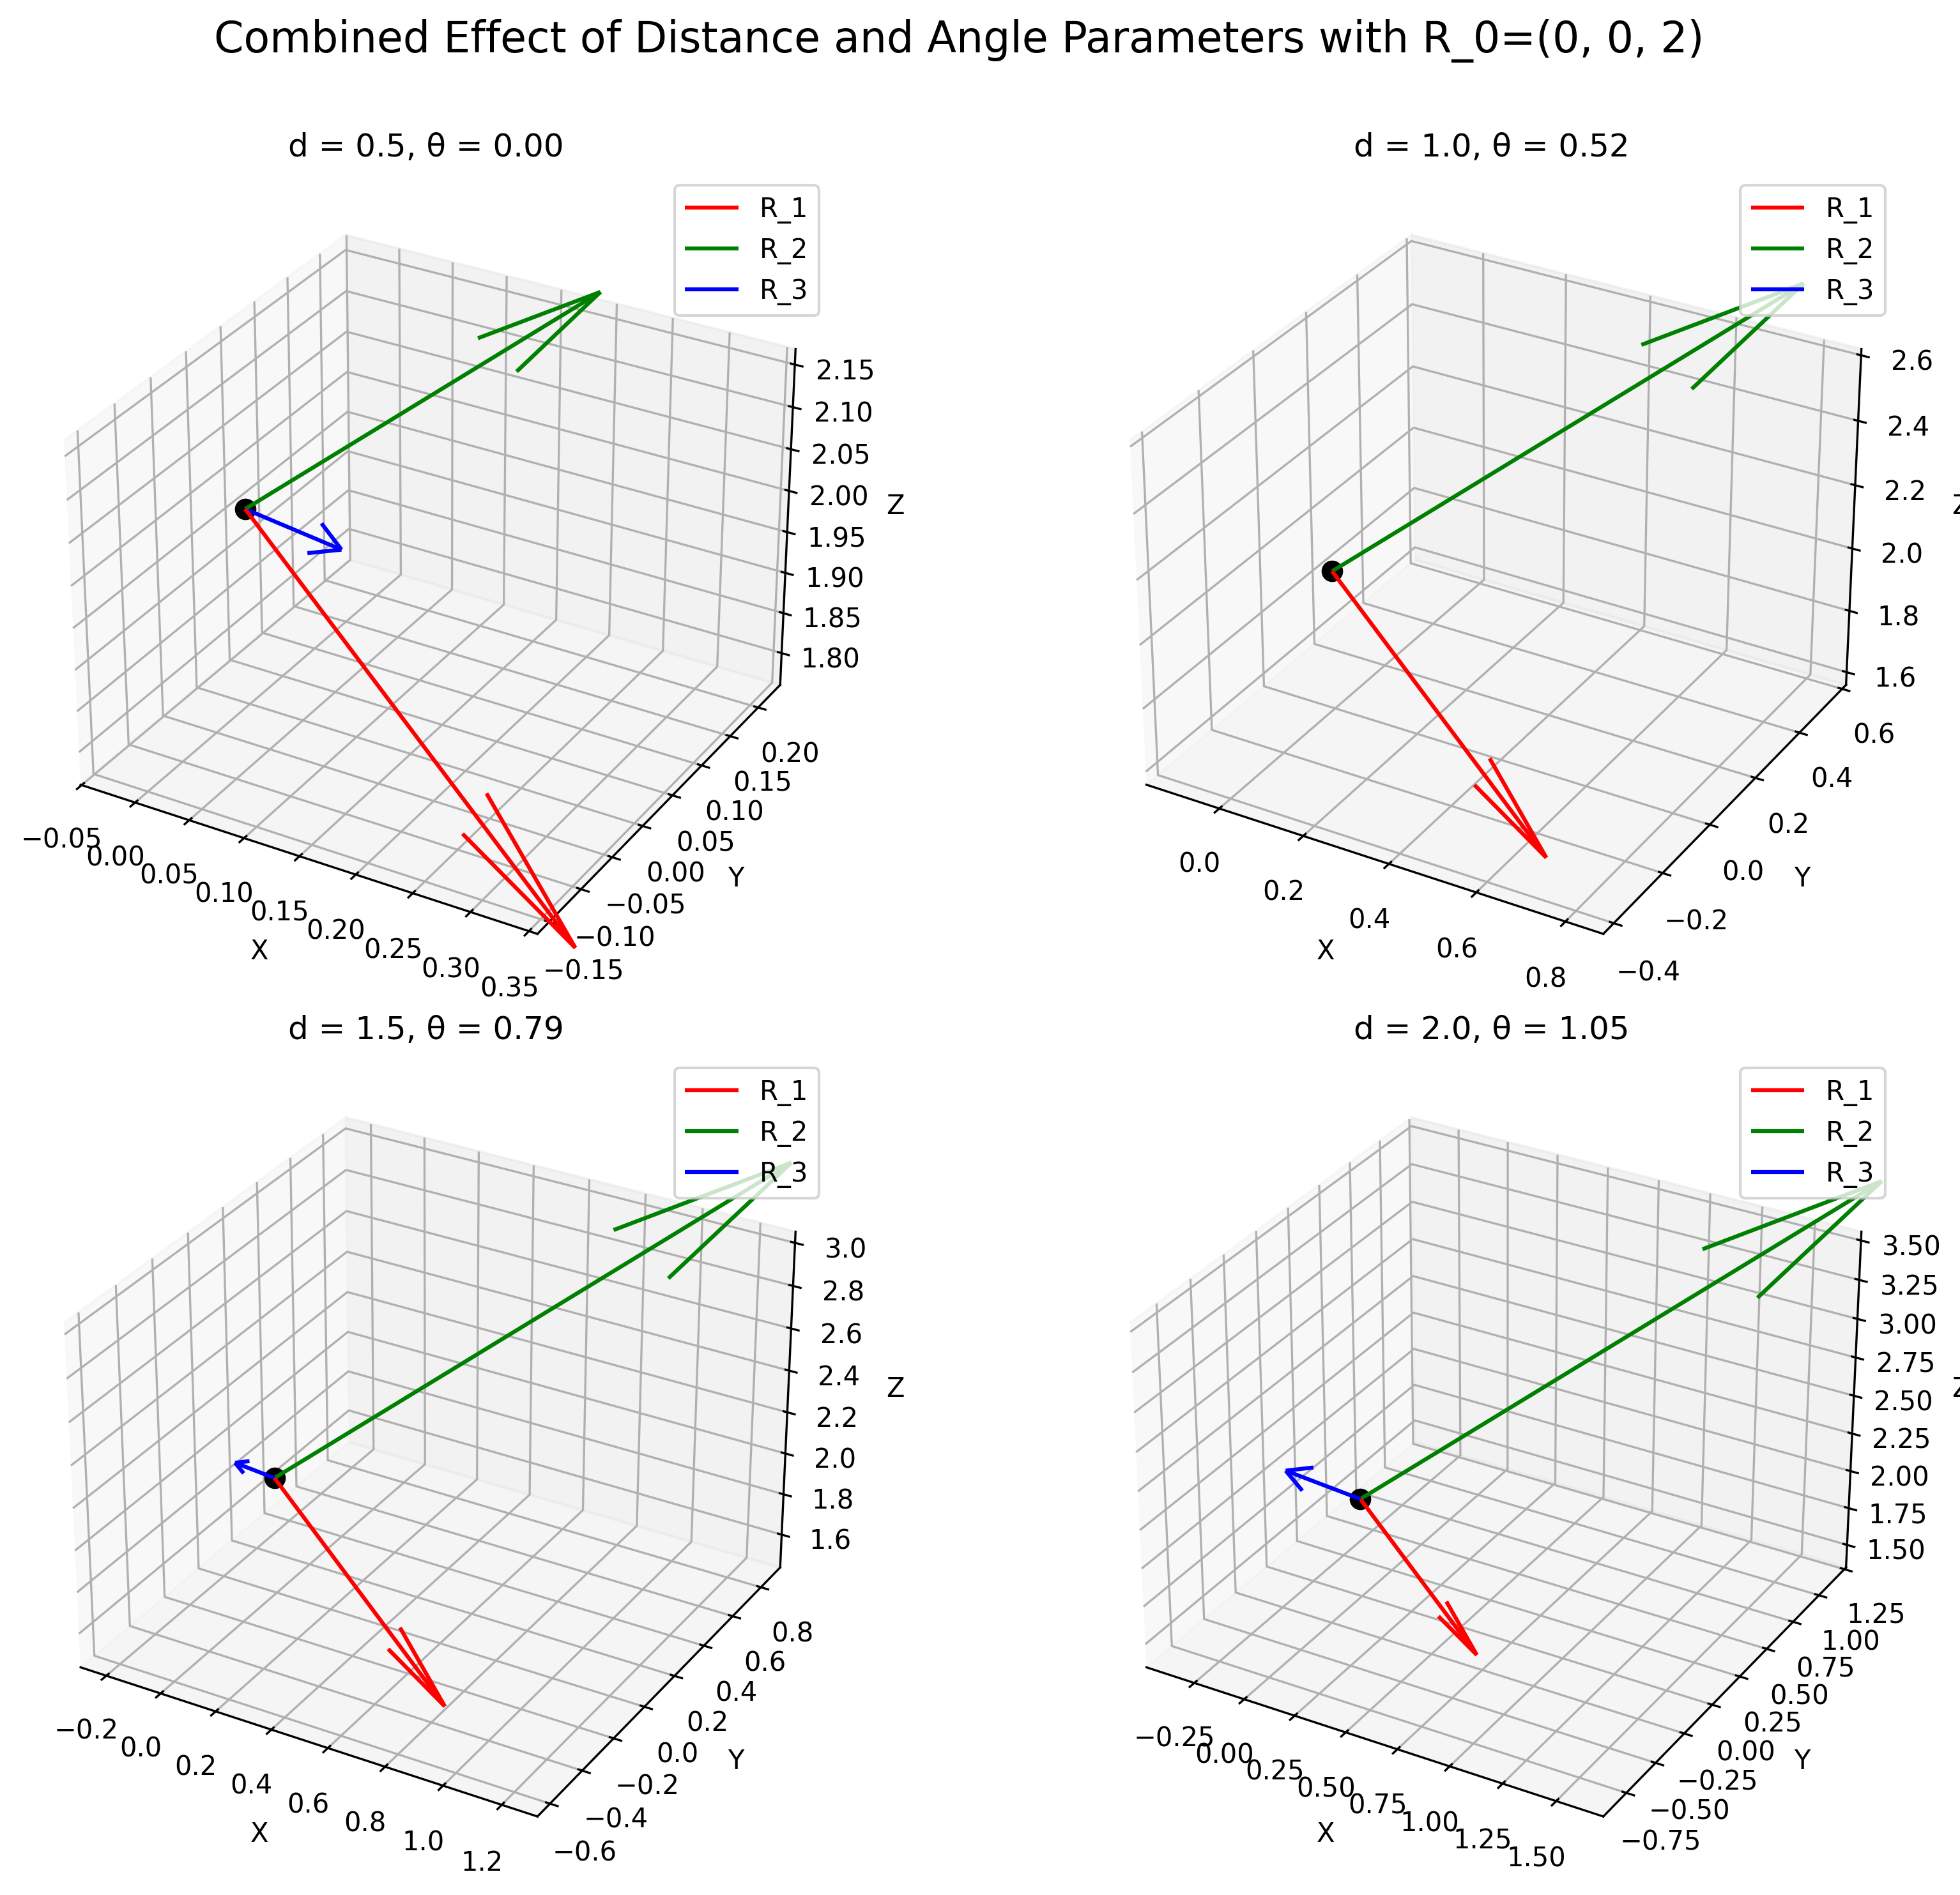
\includegraphics[width=0.9\textwidth]{figures/combined_effect_R0_0_0_2.png}
    \caption{Combined effect of distance and angle parameters with origin at $(0,0,2)$}
    \label{fig:example_combined_effect_custom2}
\end{figure}

\subsubsection{$R_0$ Plane Projections}

The $R_0$ plane projections provide a clear view of the orthogonality of the vectors in the plane perpendicular to the origin direction. These projections use a carefully constructed orthogonal basis in the plane:

\begin{itemize}
    \item When $R_0 = (0,0,0)$, the basis vectors are derived from $R_1$ and $R_2$ after orthogonalization using the Gram-Schmidt process.
    \item For non-zero $R_0$, the basis is constructed as follows:
    \begin{itemize}
        \item The plane normal is defined as the normalized vector from the global origin to $R_0$.
        \item The first basis vector is computed as the cross product of this normal with either $[1,0,0]$ or $[0,1,0]$ (whichever is not parallel to the normal).
        \item The second basis vector is computed as the cross product of the normal with the first basis vector.
    \end{itemize}
    \item This construction ensures that both basis vectors are orthogonal to each other and lie in the plane perpendicular to the vector from the origin to $R_0$.
\end{itemize}

The projections use these basis vectors as the coordinate axes, with the origin of the projection being $R_0$. This approach provides an optimal view of the orthogonality relationships between the vectors.

\begin{figure}[H]
    \centering
    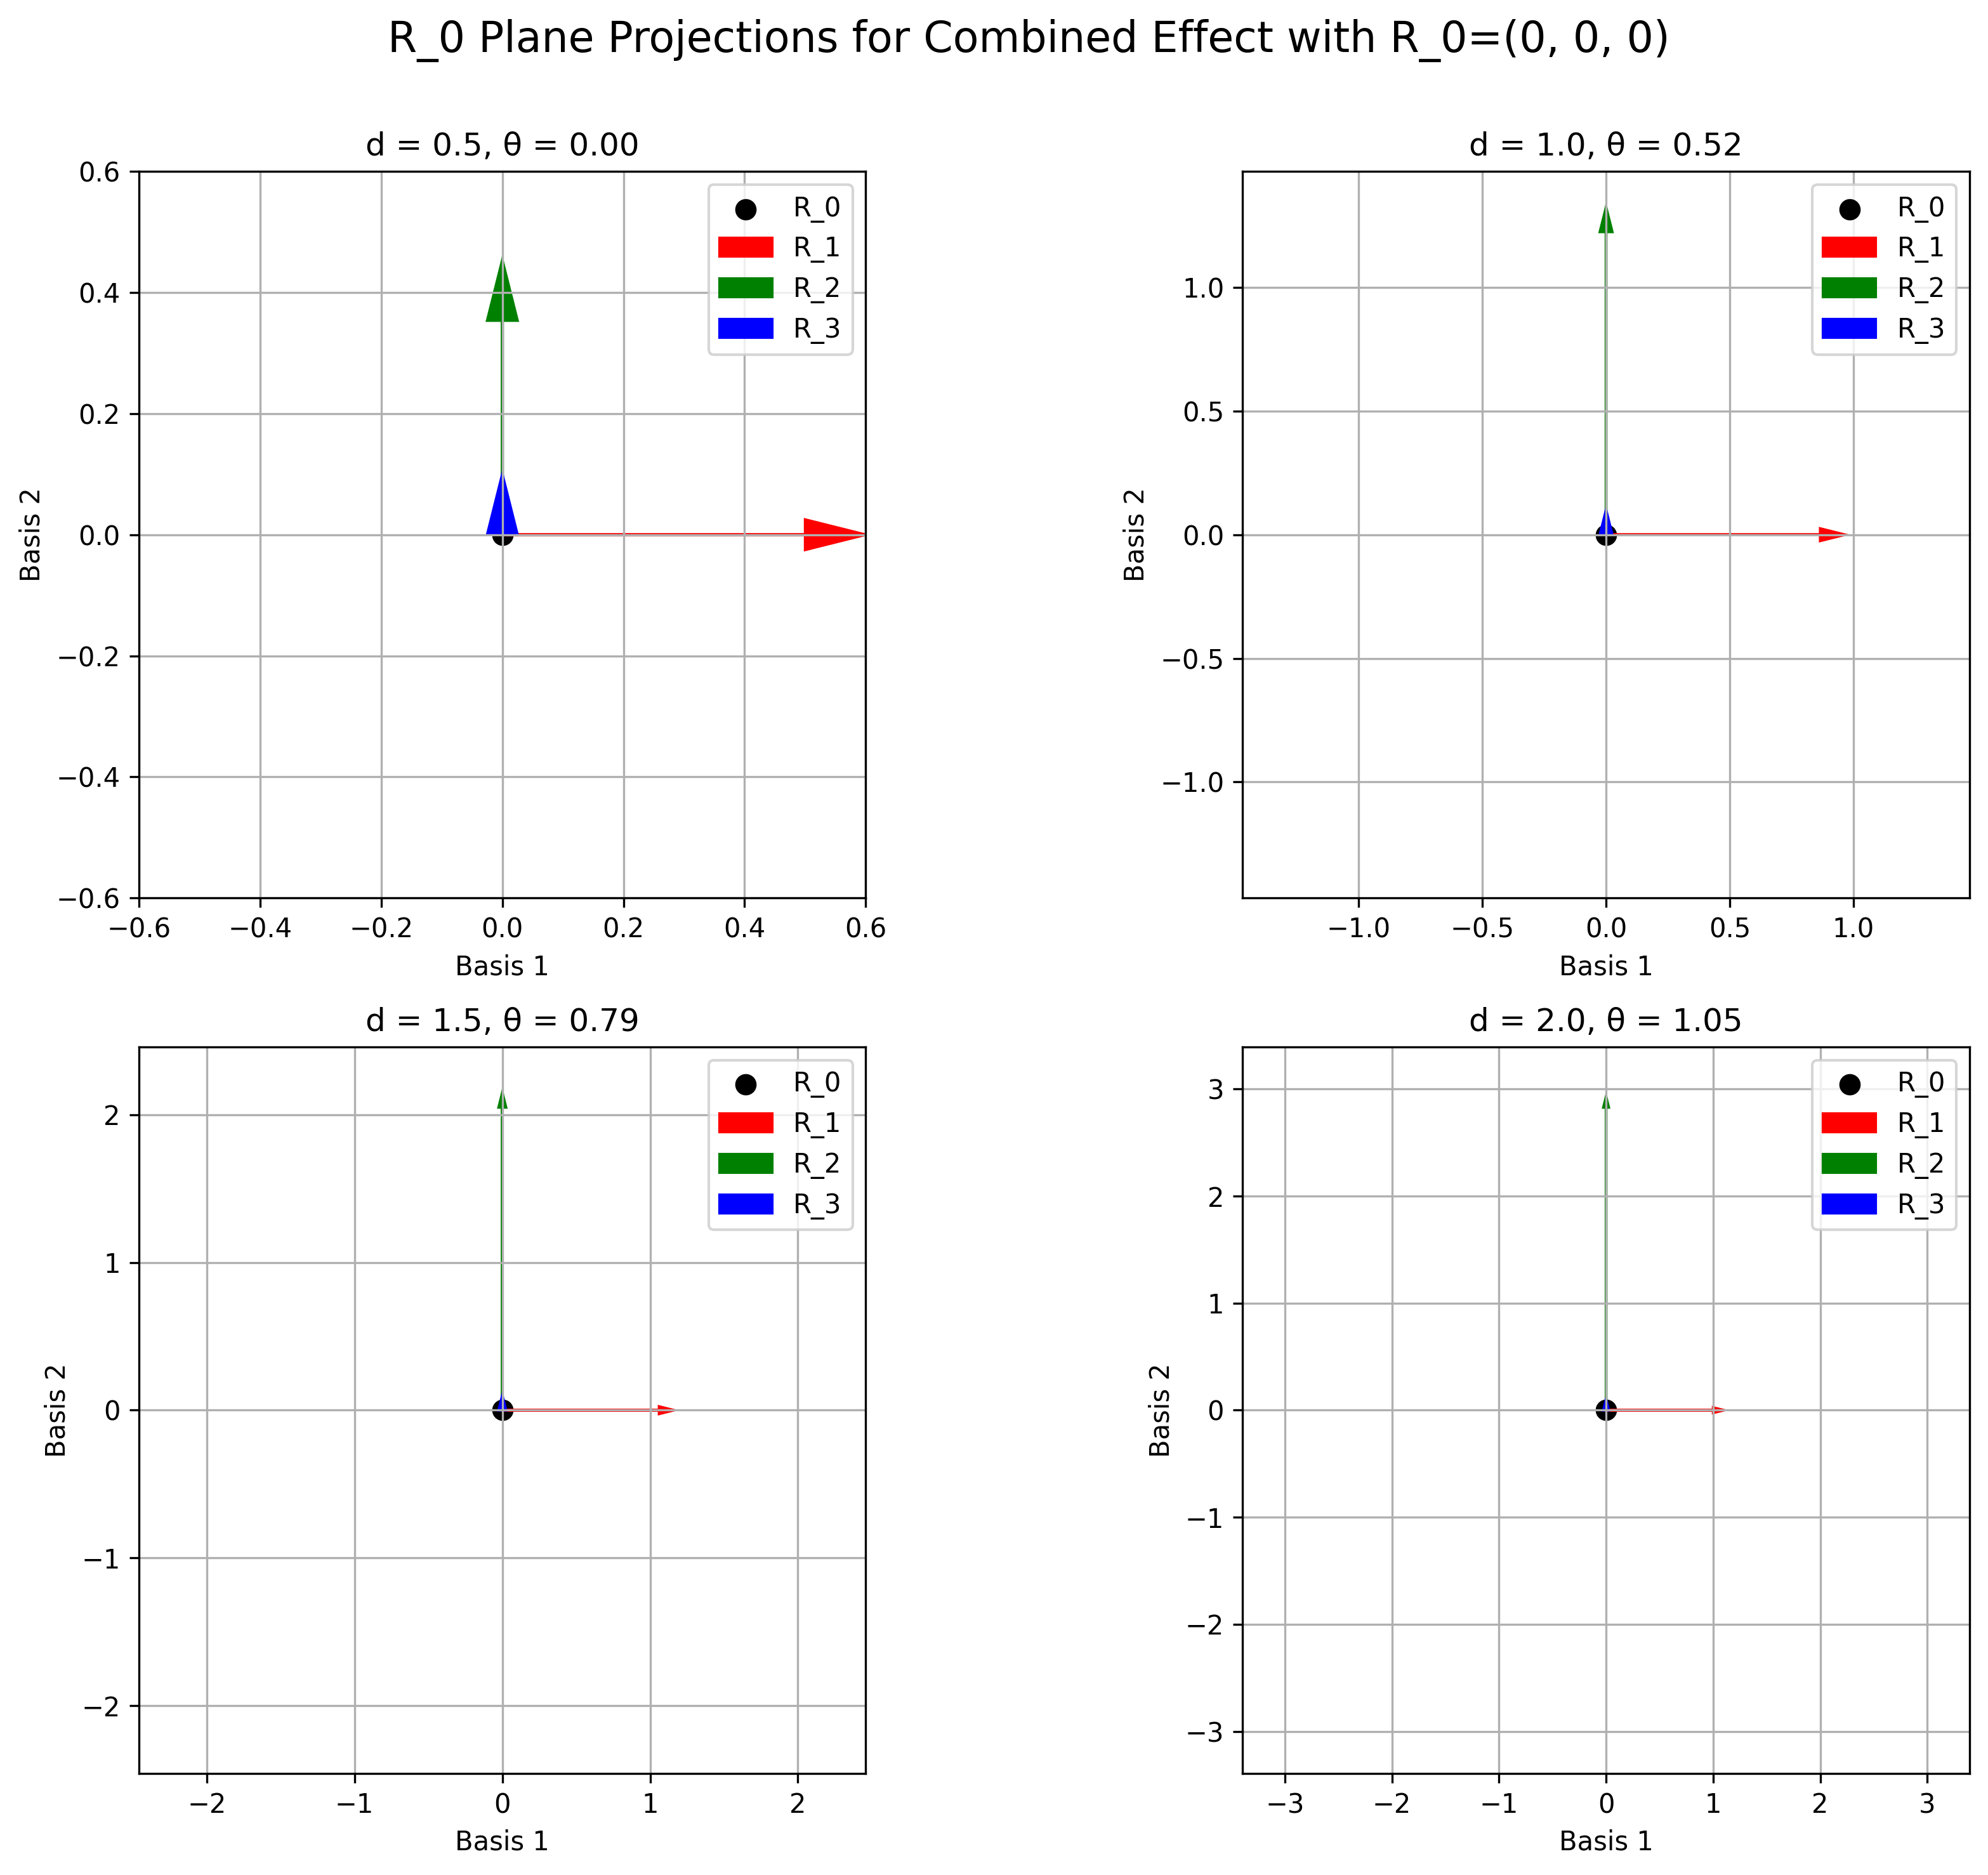
\includegraphics[width=0.9\textwidth]{figures/r0_projections_combined_effect_R0_0_0_0.png}
    \caption{$R_0$ plane projections for combined effect with origin at $(0,0,0)$}
    \label{fig:example_r0_projections_default}
\end{figure}

\begin{figure}[H]
    \centering
    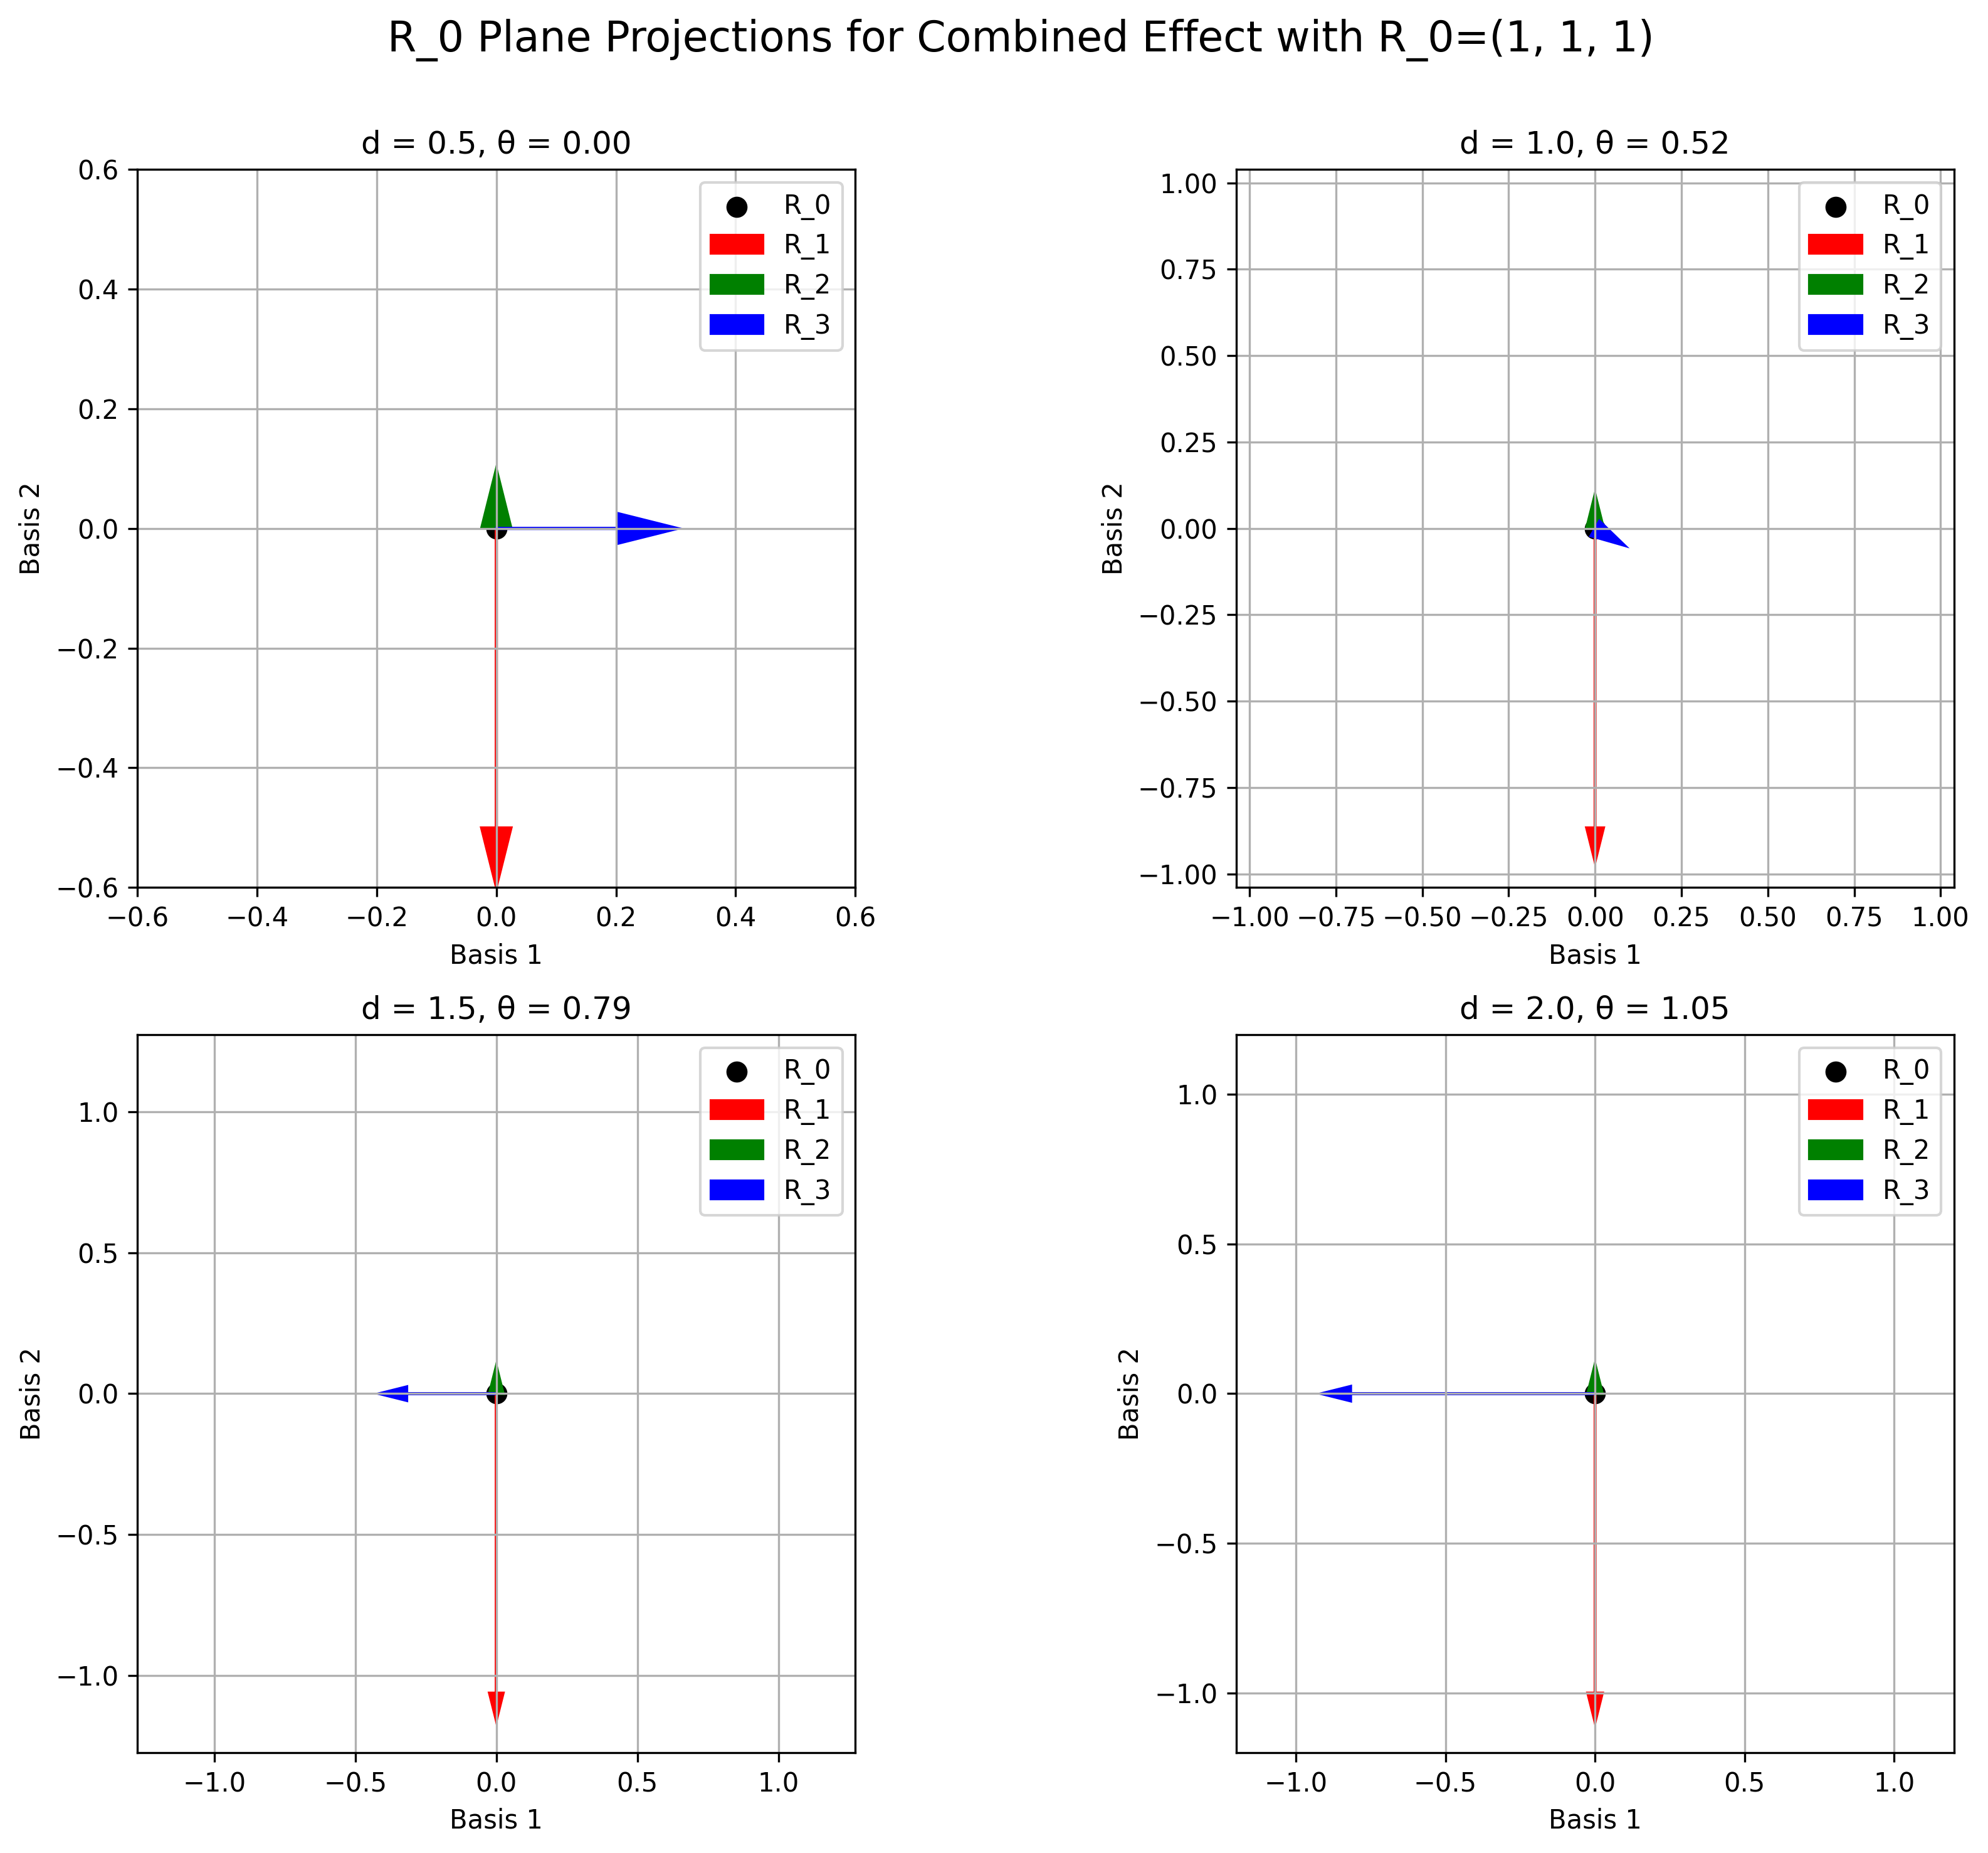
\includegraphics[width=0.9\textwidth]{figures/r0_projections_combined_effect_R0_1_1_1.png}
    \caption{$R_0$ plane projections for combined effect with origin at $(1,1,1)$}
    \label{fig:example_r0_projections_custom1}
\end{figure}

\begin{figure}[H]
    \centering
    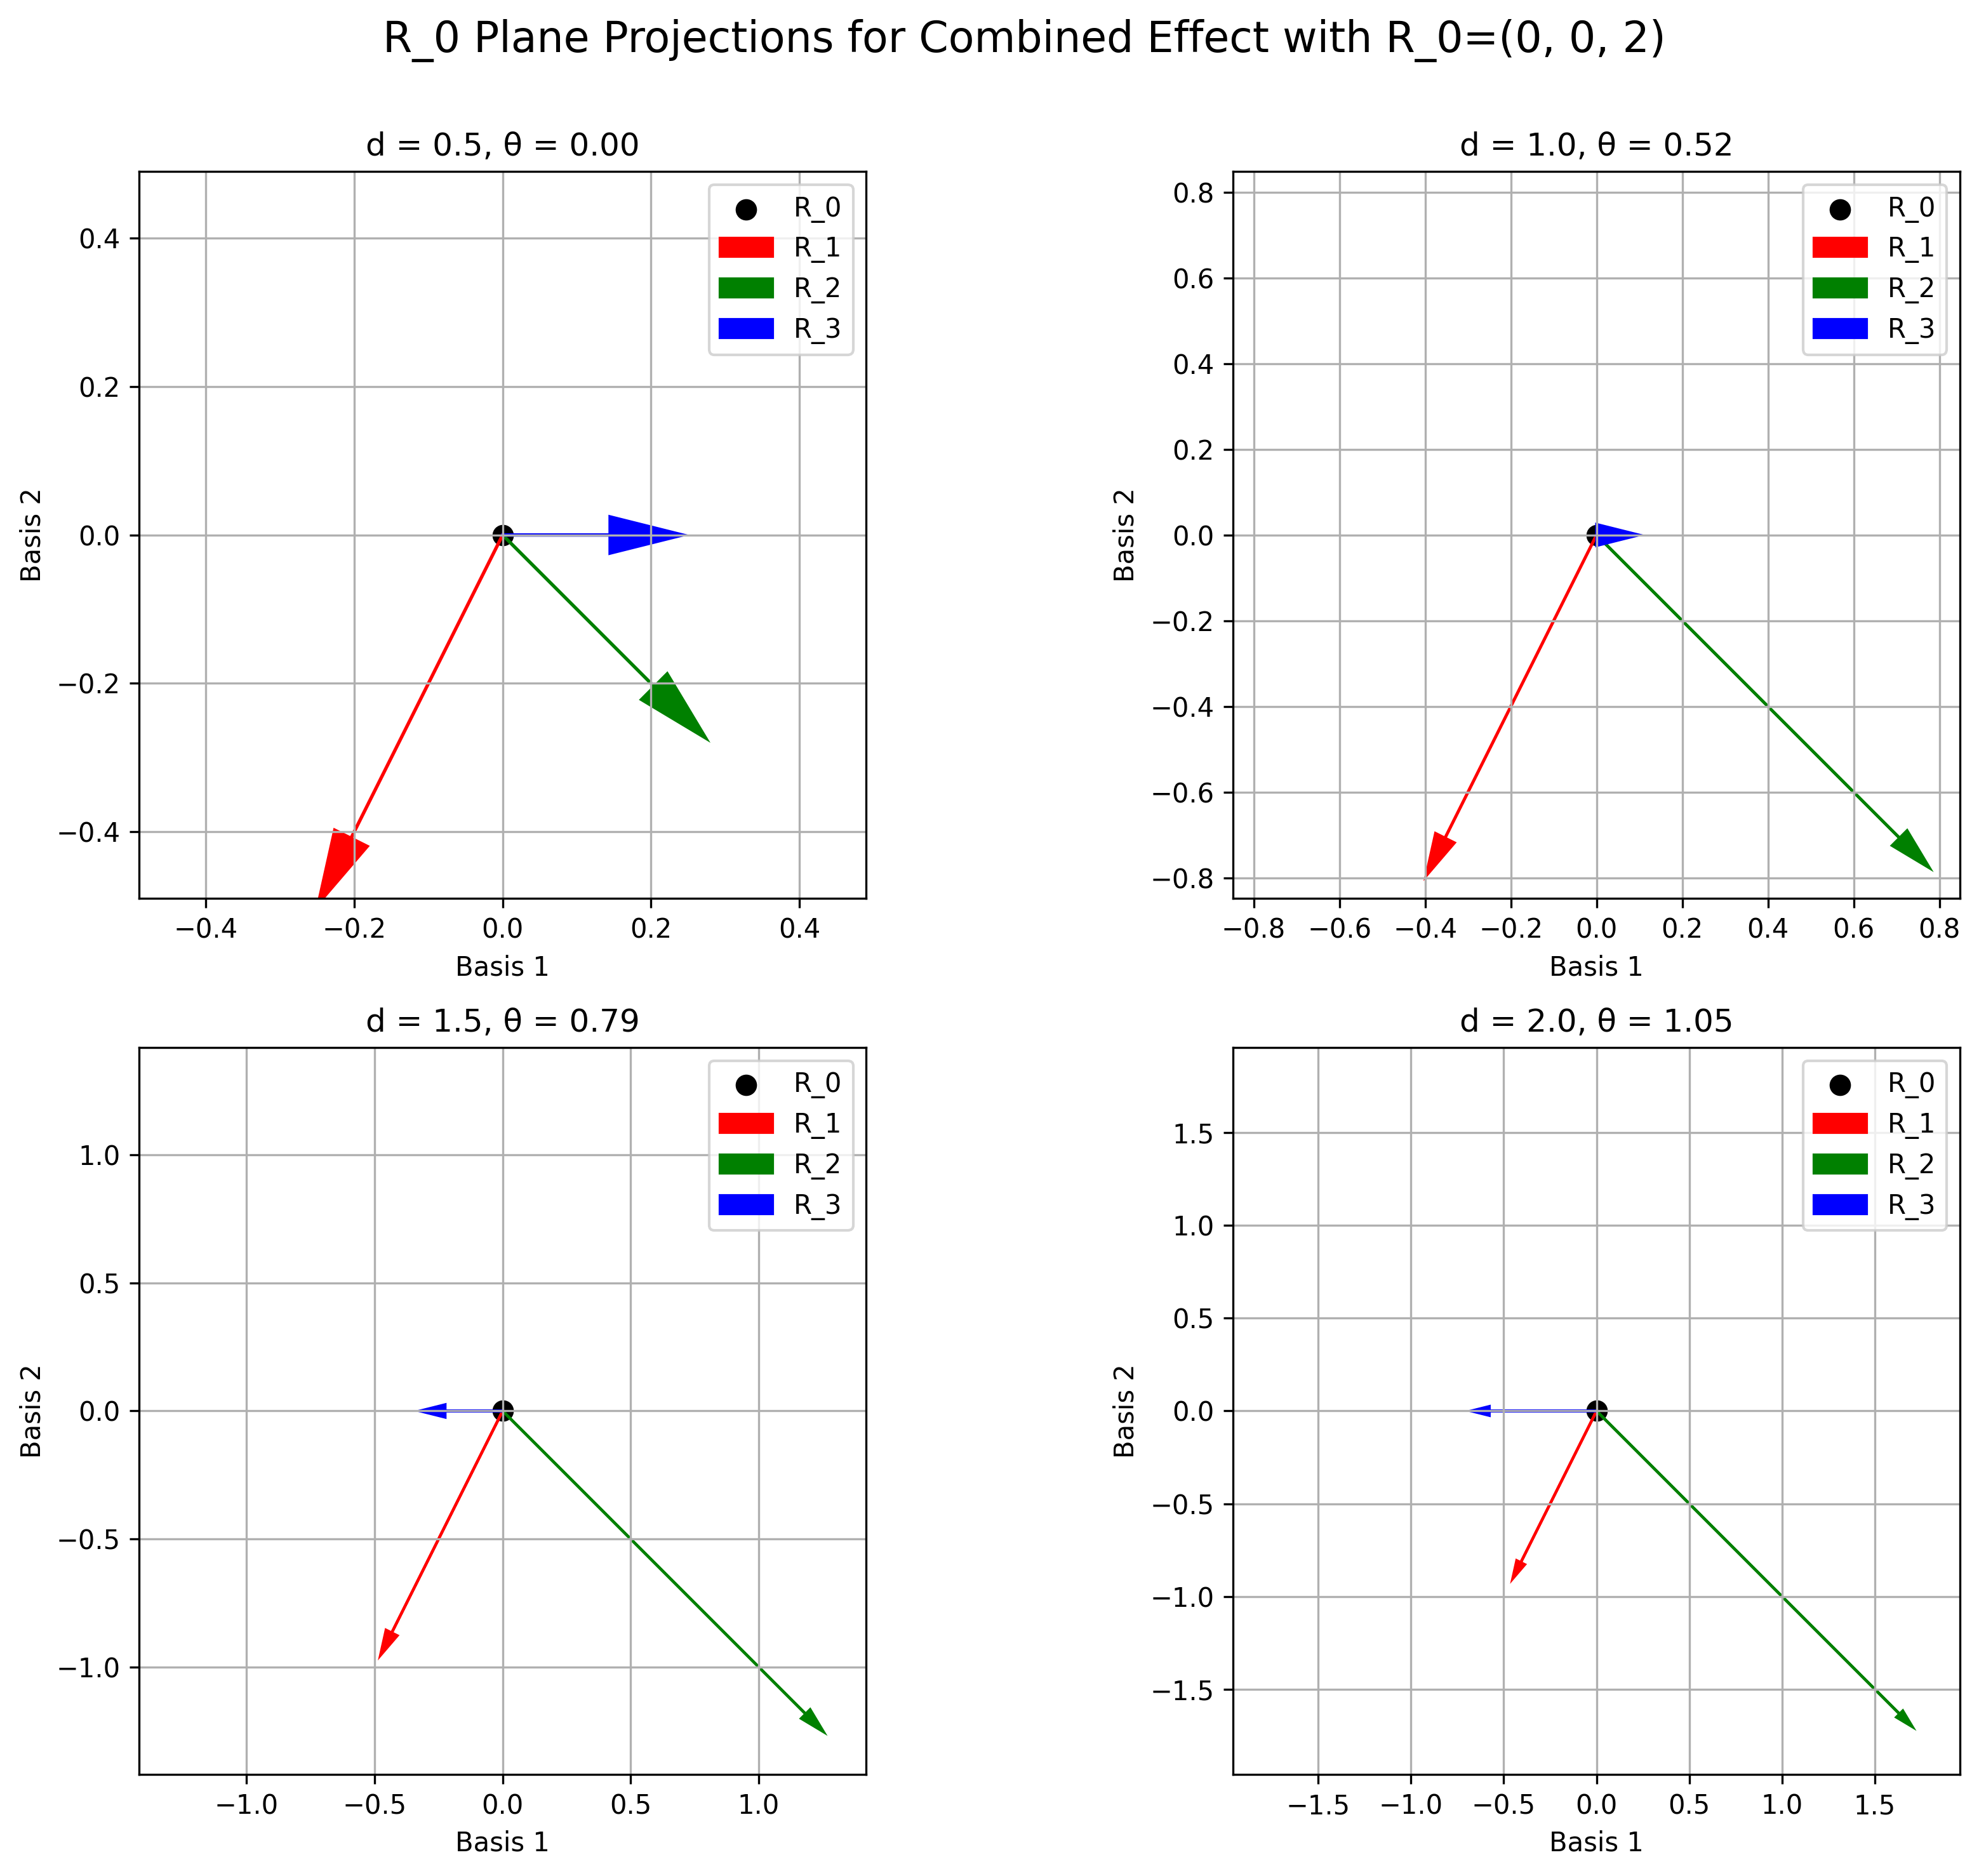
\includegraphics[width=0.9\textwidth]{figures/r0_projections_combined_effect_R0_0_0_2.png}
    \caption{$R_0$ plane projections for combined effect with origin at $(0,0,2)$}
    \label{fig:example_r0_projections_custom2}
\end{figure}

\subsubsection{Combined 3D and $R_0$ Plane Views}

The combined views show both the 3D vectors and their $R_0$ plane projections side by side, providing a comprehensive understanding of the vector relationships.

\begin{figure}[H]
    \centering
    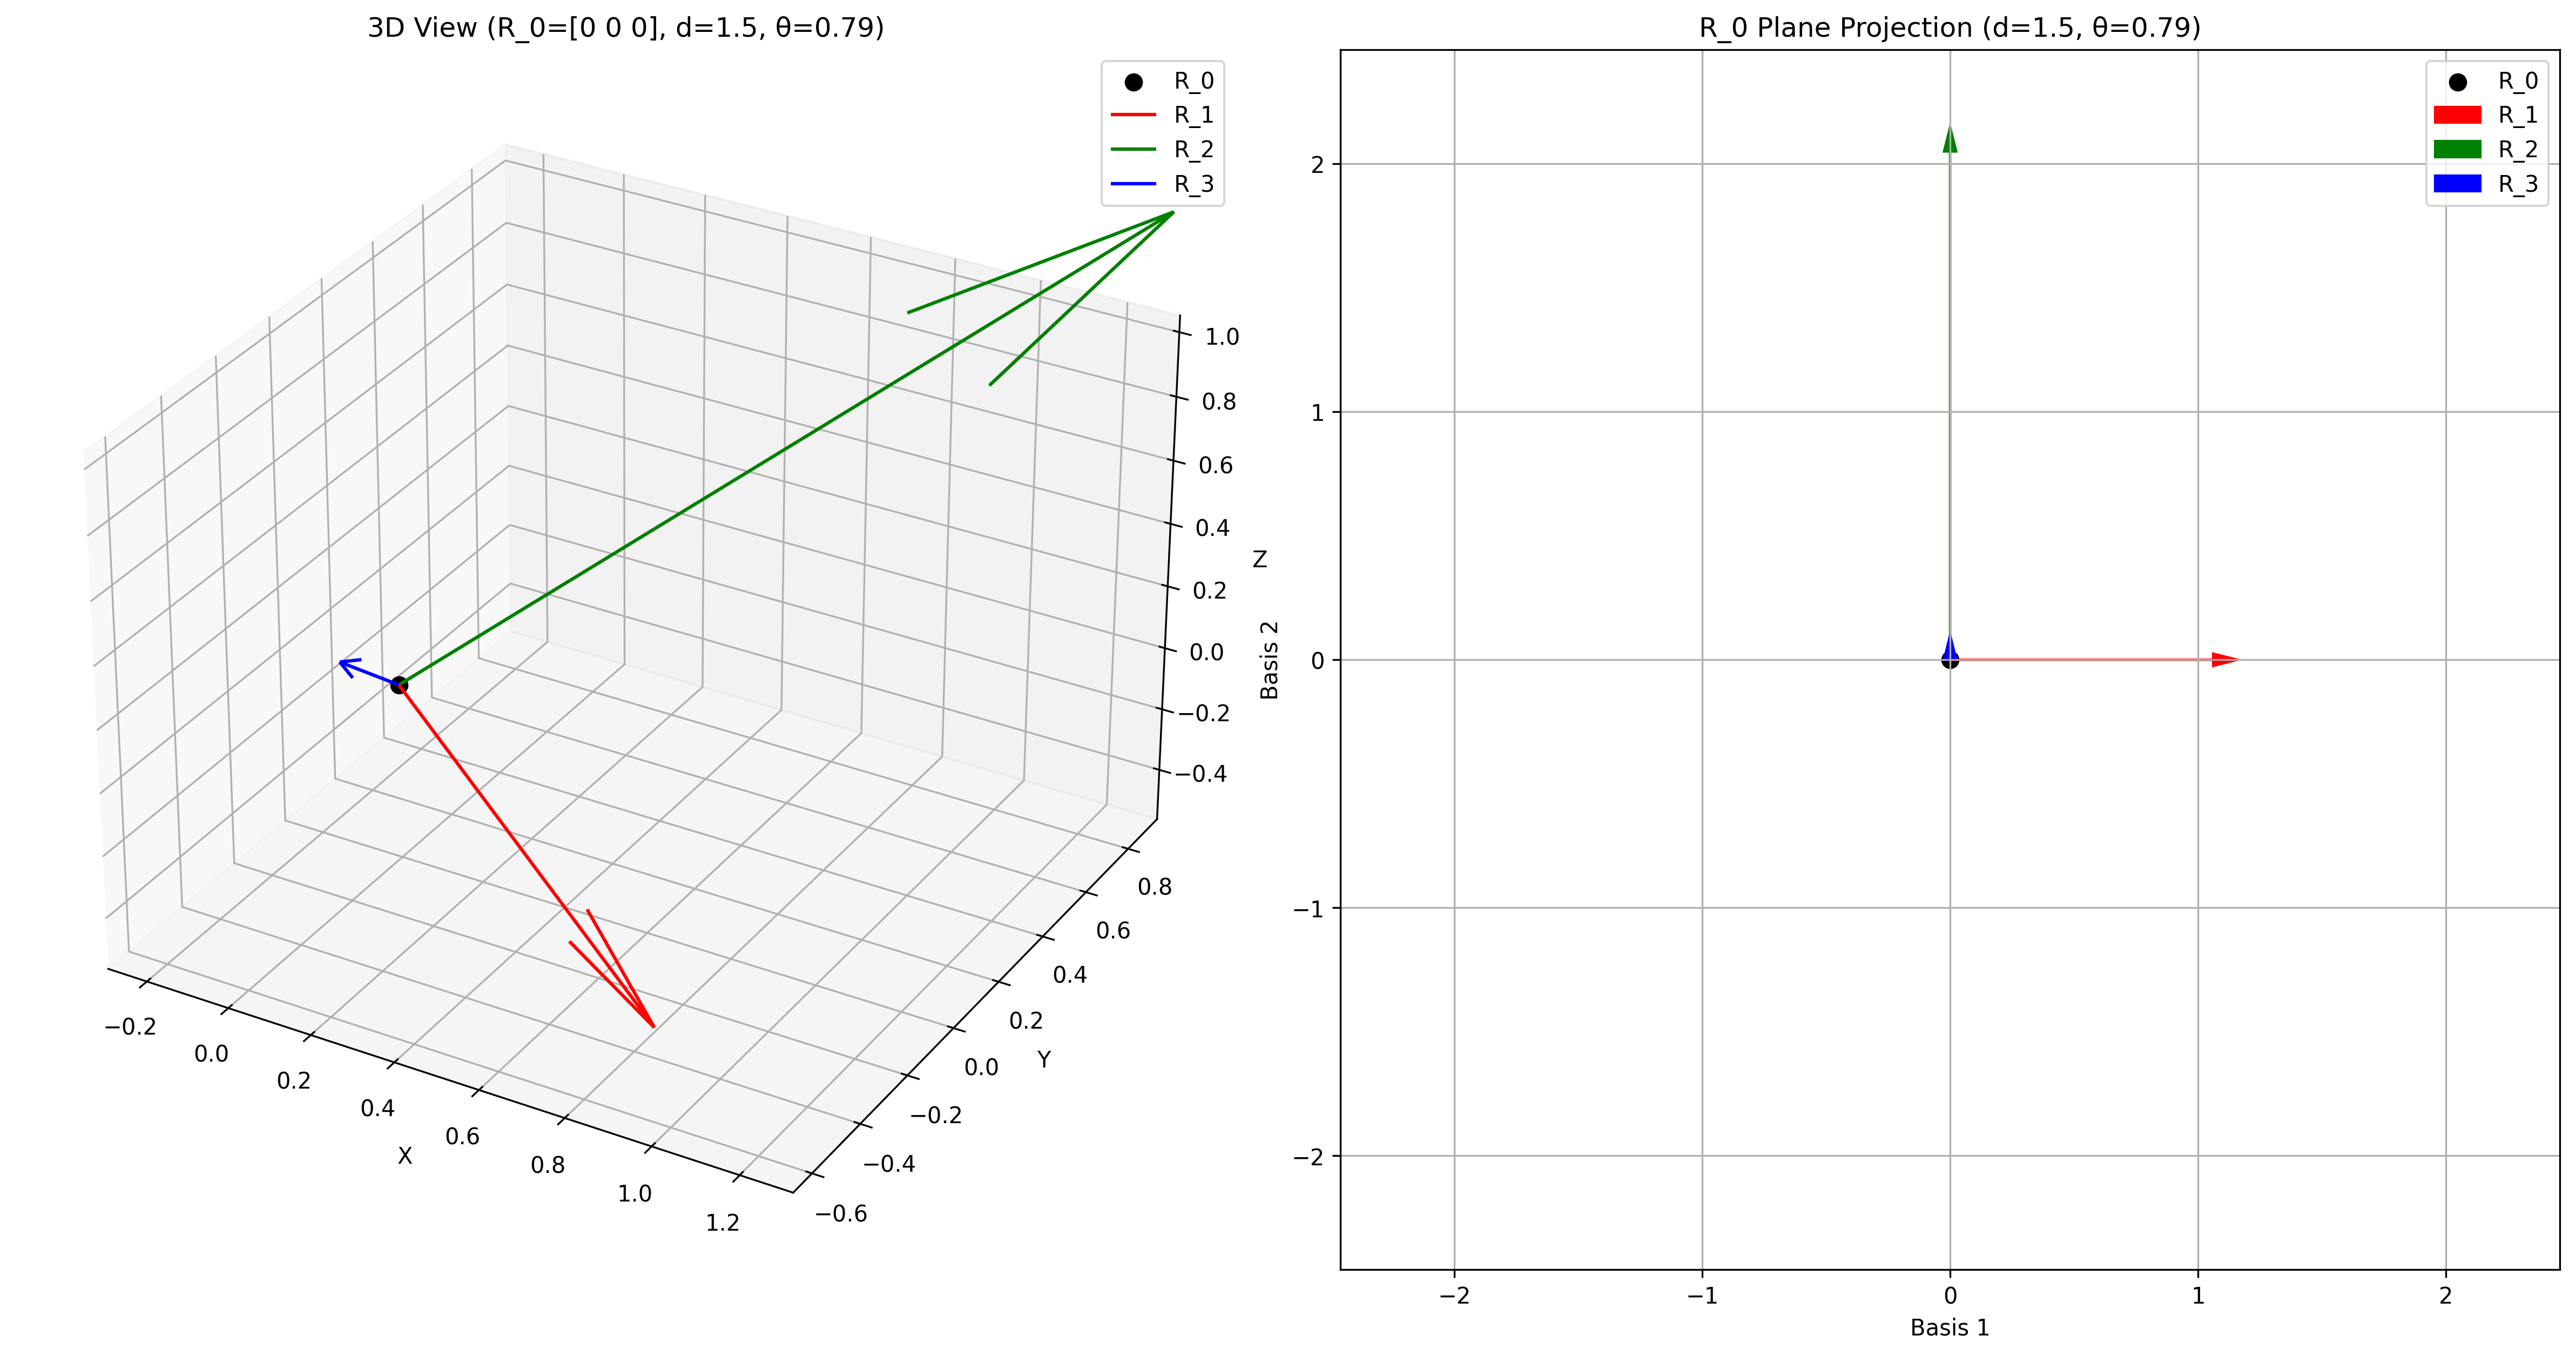
\includegraphics[width=0.9\textwidth]{figures/combined_view_R0_0_0_0_d_1p5_theta_0p79.png}
    \caption{Combined 3D and $R_0$ plane view with origin at $(0,0,0)$, $d=1.5$, $\theta=\pi/4$}
    \label{fig:example_combined_view_default}
\end{figure}

\begin{figure}[H]
    \centering
    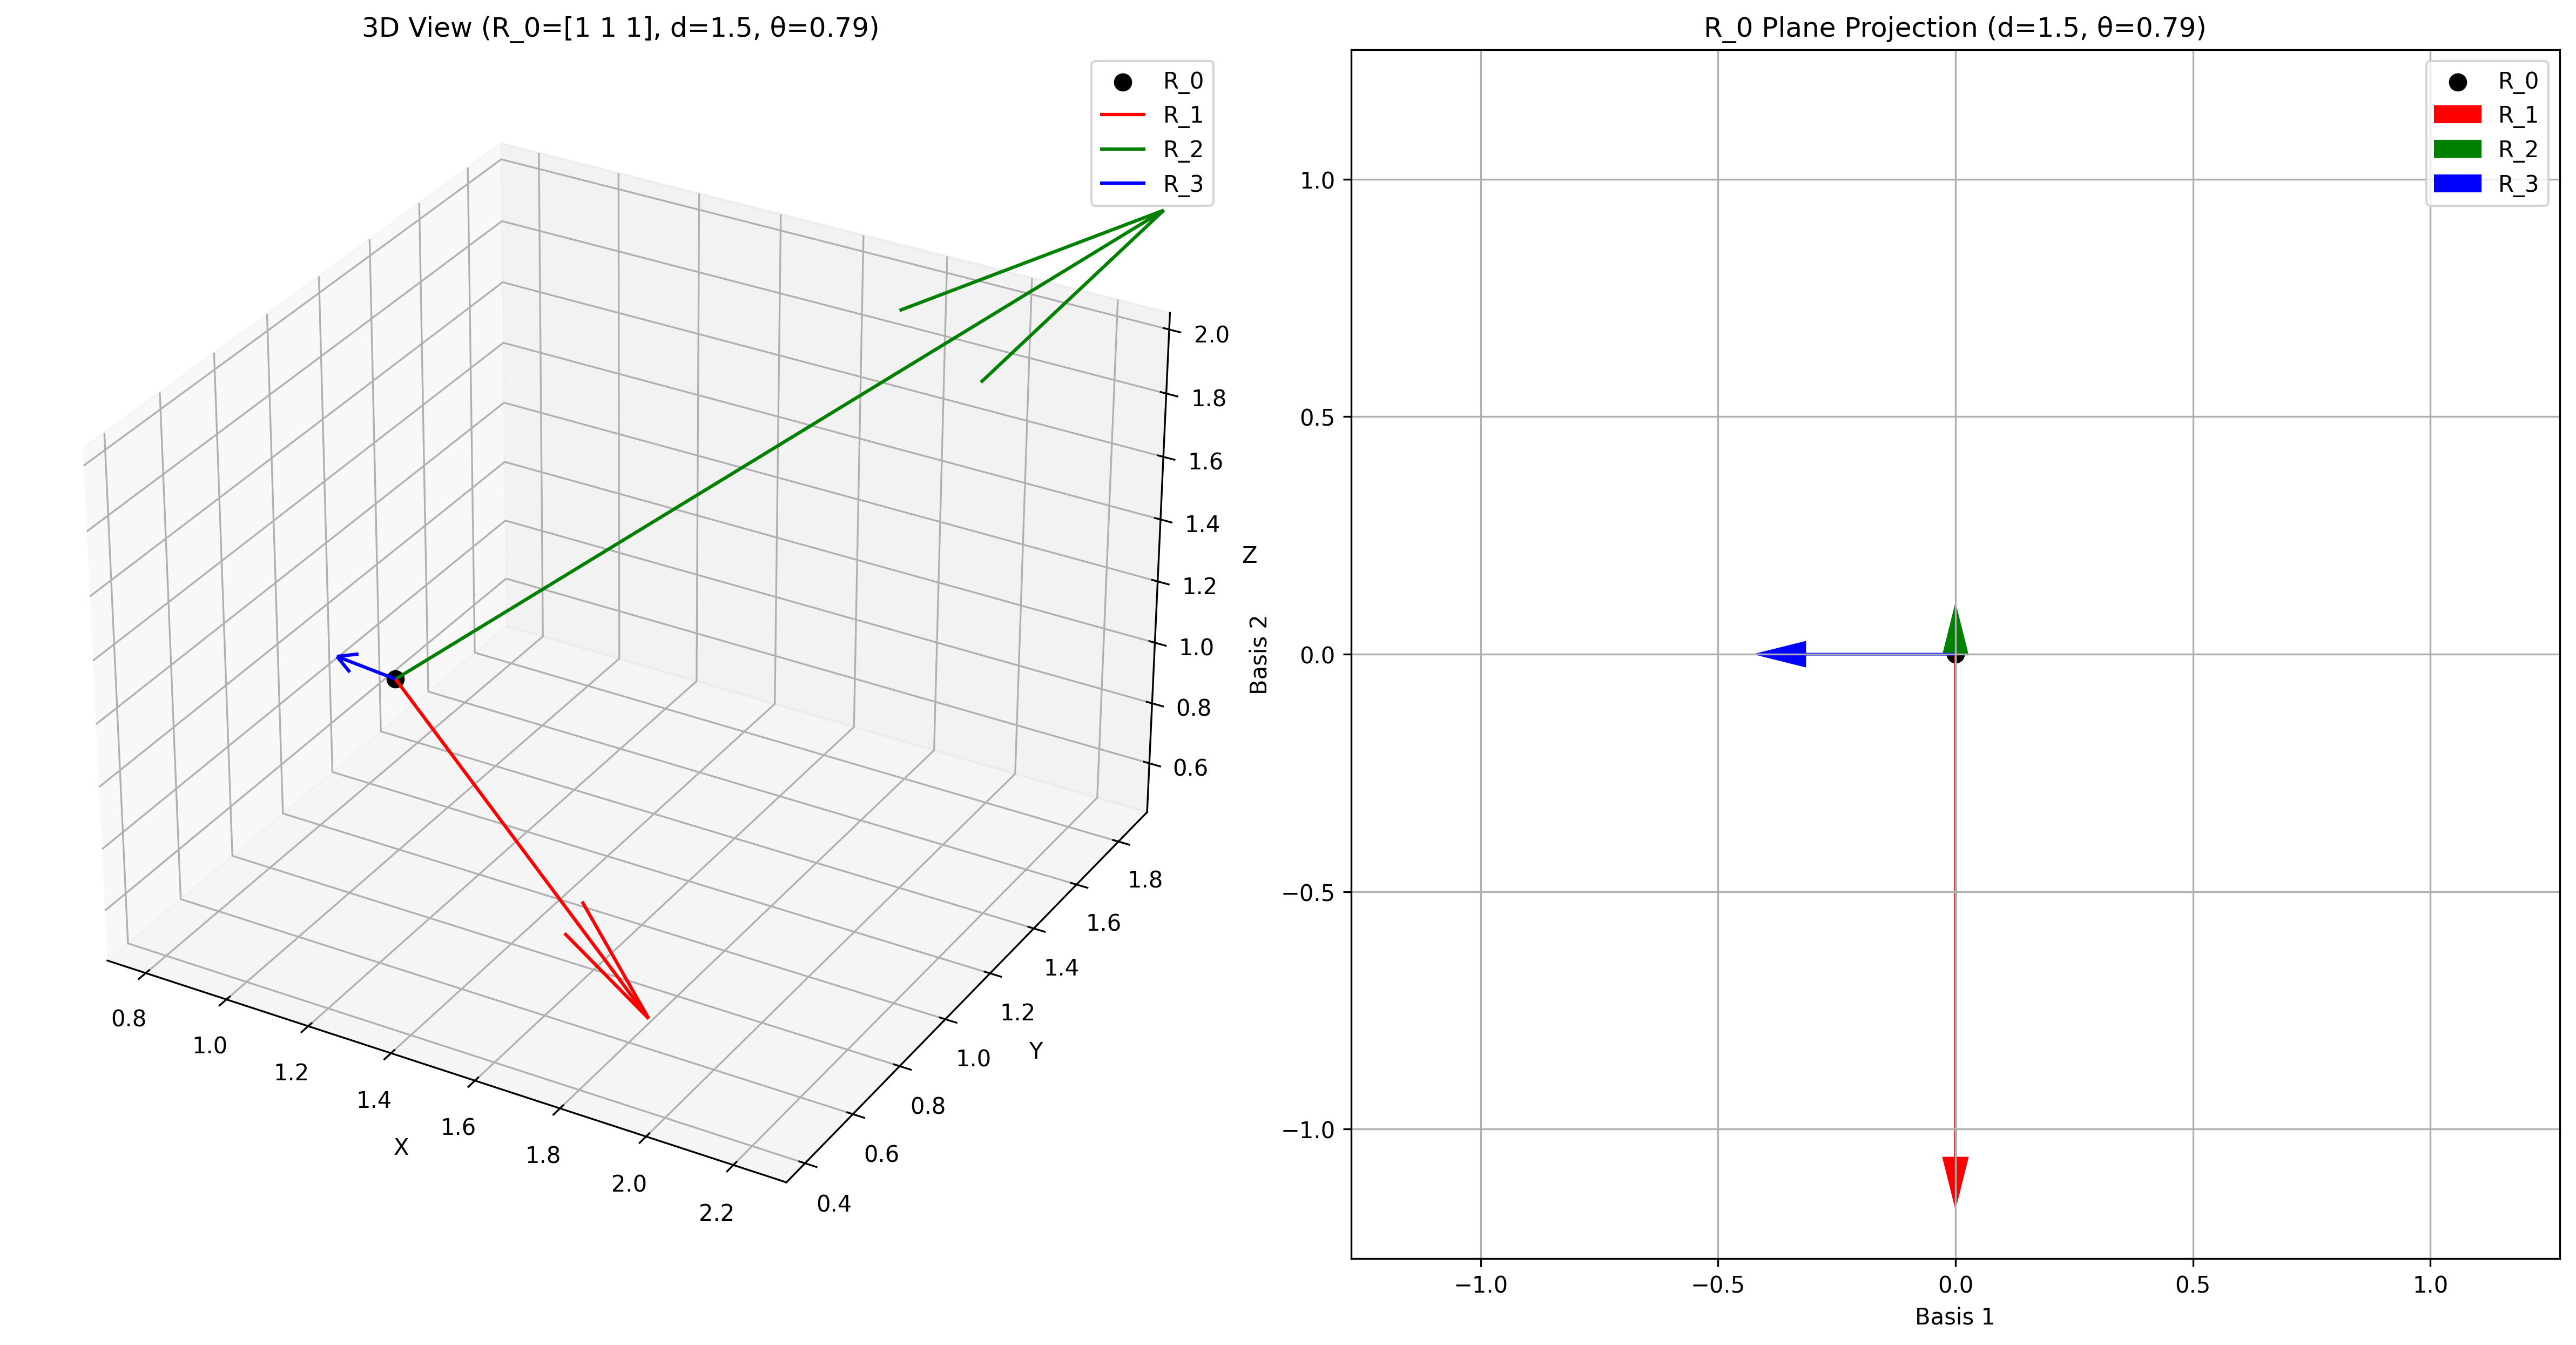
\includegraphics[width=0.9\textwidth]{figures/combined_view_R0_1_1_1_d_1p5_theta_0p79.png}
    \caption{Combined 3D and $R_0$ plane view with origin at $(1,1,1)$, $d=1.5$, $\theta=\pi/4$}
    \label{fig:example_combined_view_custom1}
\end{figure}

\begin{figure}[H]
    \centering
    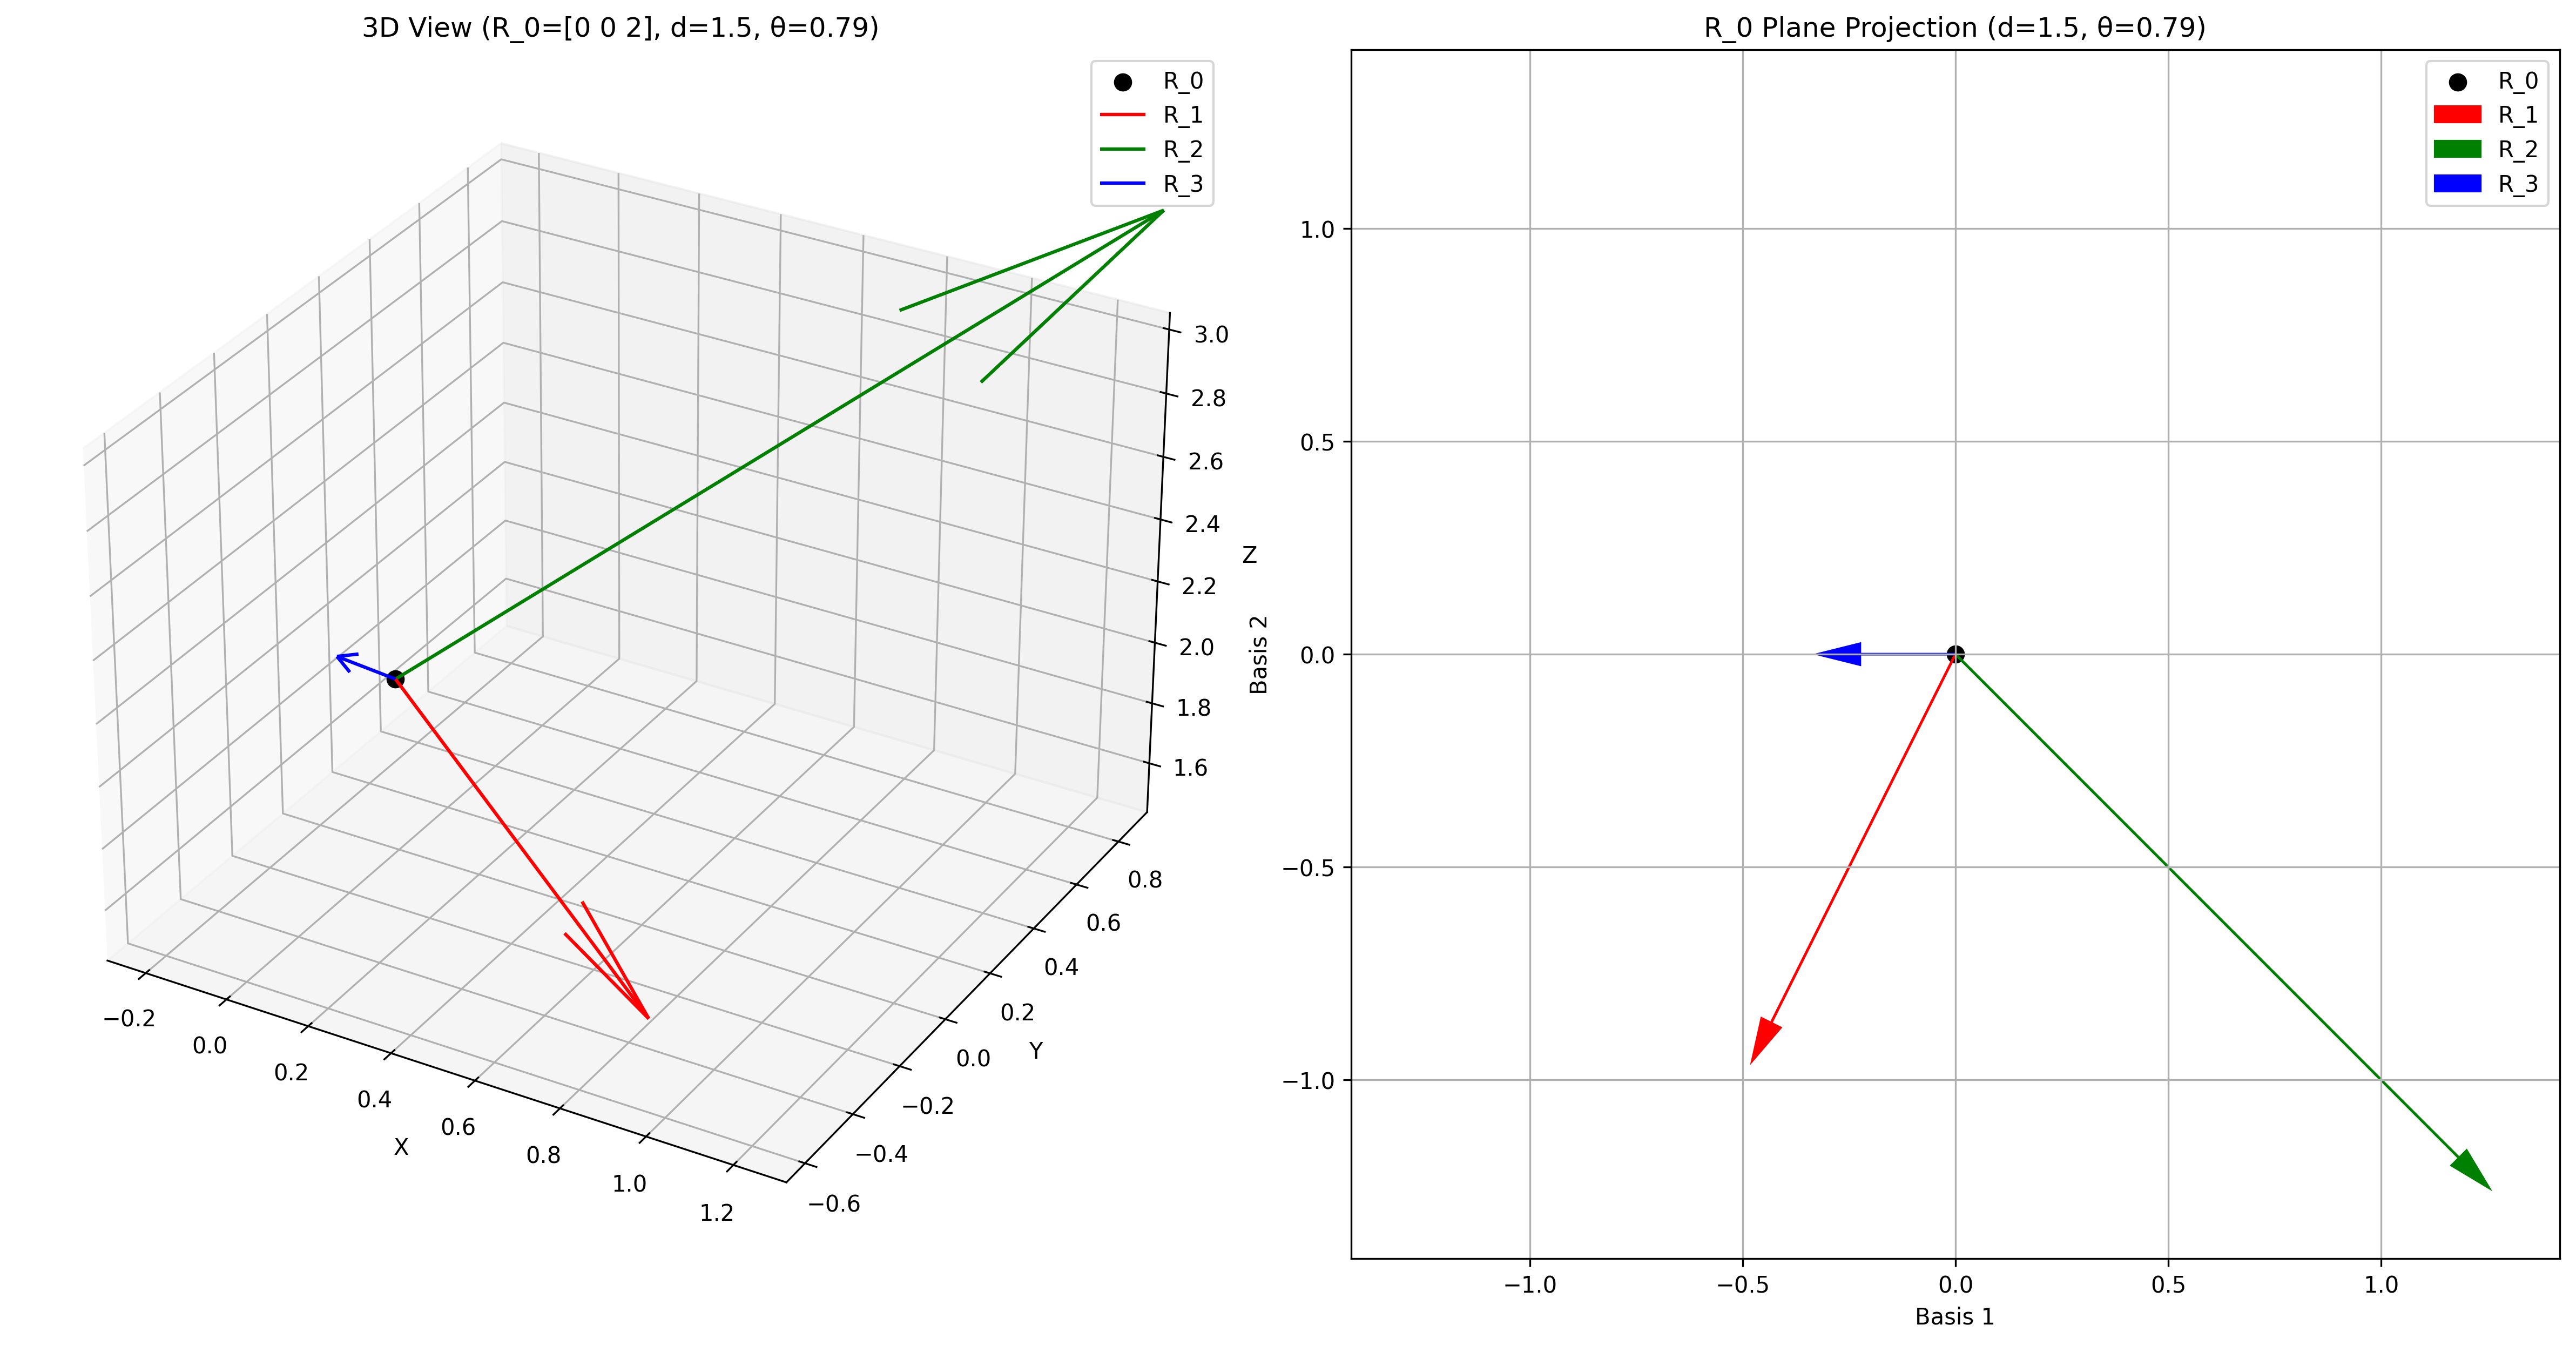
\includegraphics[width=0.9\textwidth]{figures/combined_view_R0_0_0_2_d_1p5_theta_0p79.png}
    \caption{Combined 3D and $R_0$ plane view with origin at $(0,0,2)$, $d=1.5$, $\theta=\pi/4$}
    \label{fig:example_combined_view_custom2}
\end{figure}

\textbf{Effect of Origin and Combined Parameters:} The origin parameter $\vec{R}_0$ shifts the entire vector system, preserving the orthogonality of the displacement vectors. Different origin points result in different positions of the vectors in space. The figures above demonstrate how different combinations of distance and angle parameters affect the vector visualization for each origin point. This illustrates the flexibility of the generalized orthogonal vectors implementation in creating various vector configurations.

\subsection{Summary of Results}

The example results demonstrate that the Generalized Orthogonal Vectors Generator and Visualizer successfully generates and visualizes orthogonal vectors for various configurations. The vectors are confirmed to be orthogonal by calculating their dot products, which are all zero (within numerical precision).

The visualizations show the vectors in both 3D and 2D projections, providing different perspectives on their spatial relationships. The effects of the distance parameter, angle parameter, and origin on the vector system are also demonstrated.
